%% Run LaTeX on this file several times to get Table of Contents,
%% cross-references, and citations.

\documentclass[11pt]{book}
\usepackage{gvv-book}
\usepackage{gvv}
%\usepackage{Wiley-AuthoringTemplate}
\usepackage[sectionbib,authoryear]{natbib}% for name-date citation comment the below line
%\usepackage[sectionbib,numbers]{natbib}% for numbered citation comment the above line

%%********************************************************************%%
%%       How many levels of section head would you like numbered?     %%
%% 0= no section numbers, 1= section, 2= subsection, 3= subsubsection %%
\setcounter{secnumdepth}{3}
%%********************************************************************%%
%%**********************************************************************%%
%%     How many levels of section head would you like to appear in the  %%
%%				Table of Contents?			%%
%% 0= chapter, 1= section, 2= subsection, 3= subsubsection titles.	%%
\setcounter{tocdepth}{2}
%%**********************************************************************%%

%\includeonly{ch01}
\makeindex

\begin{document}

\frontmatter
%%%%%%%%%%%%%%%%%%%%%%%%%%%%%%%%%%%%%%%%%%%%%%%%%%%%%%%%%%%%%%%%
%% Title Pages
%% Wiley will provide title and copyright page, but you can make
%% your own titlepages if you'd like anyway
%% Setting up title pages, type in the appropriate names here:

\booktitle{JEE}

\subtitle{Previous Year Questions}

\AuAff{G. V. V. Sharma}


%% \\ will start a new line.
%% You may add \affil{} for affiliation, ie,
%\authors{Robert M. Groves\\
%\affil{Universitat de les Illes Balears}
%Floyd J. Fowler, Jr.\\
%\affil{University of New Mexico}
%}

%% Print Half Title and Title Page:
%\halftitlepage
\titlepage

%%%%%%%%%%%%%%%%%%%%%%%%%%%%%%%%%%%%%%%%%%%%%%%%%%%%%%%%%%%%%%%%
%% Copyright Page

\begin{copyrightpage}{2024}
%Title, etc
\end{copyrightpage}

% Note, you must use \ to start indented lines, ie,
% 
% \begin{copyrightpage}{2004}
% Survey Methodology / Robert M. Groves . . . [et al.].
% \       p. cm.---(Wiley series in survey methodology)
% \    ``Wiley-Interscience."
% \    Includes bibliographical references and index.
% \    ISBN 0-471-48348-6 (pbk.)
% \    1. Surveys---Methodology.  2. Social 
% \  sciences---Research---Statistical methods.  I. Groves, Robert M.  II. %
% Series.\\

% HA31.2.S873 2004
% 001.4'33---dc22                                             2004044064
% \end{copyrightpage}

%%%%%%%%%%%%%%%%%%%%%%%%%%%%%%%%%%%%%%%%%%%%%%%%%%%%%%%%%%%%%%%%
%% Only Dedication (optional) 

%\dedication{To my parents}

\tableofcontents

%\listoffigures %optional
%\listoftables  %optional

%% or Contributor Page for edited books
%% before \tableofcontents

%%%%%%%%%%%%%%%%%%%%%%%%%%%%%%%%%%%%%%%%%%%%%%%%%%%%%%%%%%%%%%%%
%  Contributors Page for Edited Book
%%%%%%%%%%%%%%%%%%%%%%%%%%%%%%%%%%%%%%%%%%%%%%%%%%%%%%%%%%%%%%%%

% If your book has chapters written by different authors,
% you'll need a Contributors page.

% Use \begin{contributors}...\end{contributors} and
% then enter each author with the \name{} command, followed
% by the affiliation information.

% \begin{contributors}
% \name{Masayki Abe,} Fujitsu Laboratories Ltd., Fujitsu Limited, Atsugi, Japan
%
% \name{L. A. Akers,} Center for Solid State Electronics Research, Arizona State University, Tempe, Arizona
%
% \name{G. H. Bernstein,} Department of Electrical and Computer Engineering, University of Notre Dame, Notre Dame, South Bend, Indiana; formerly of
% Center for Solid State Electronics Research, Arizona
% State University, Tempe, Arizona 
% \end{contributors}

%%%%%%%%%%%%%%%%%%%%%%%%%%%%%%%%%%%%%%%%%%%%%%%%%%%%%%%%%%%%%%%%
% Optional Foreword:

%\begin{foreword}
%\lipsum[1-2]
%\end{foreword}

%%%%%%%%%%%%%%%%%%%%%%%%%%%%%%%%%%%%%%%%%%%%%%%%%%%%%%%%%%%%%%%%
% Optional Preface:

%\begin{preface}
%\lipsum[1-1]
%\prefaceauthor{}
%\where{place\\
% date}
%\end{preface}

% ie,
% \begin{preface}
% This is an example preface.
% \prefaceauthor{R. K. Watts}
% \where{Durham, North Carolina\\
% September, 2004}

%%%%%%%%%%%%%%%%%%%%%%%%%%%%%%%%%%%%%%%%%%%%%%%%%%%%%%%%%%%%%%%%
% Optional Acknowledgments:

%\acknowledgments
%\lipsum[1-2]
%\authorinitials{I. R. S.}  

%%%%%%%%%%%%%%%%%%%%%%%%%%%%%%%%
%% Glossary Type of Environment:

% \begin{glossary}
% \term{<term>}{<description>}
% \end{glossary}

%%%%%%%%%%%%%%%%%%%%%%%%%%%%%%%%
%\begin{acronyms}
%\acro{ASTA}{Arrivals See Time Averages}
%\acro{BHCA}{Busy Hour Call Attempts}
%\acro{BR}{Bandwidth Reservation}
%\acro{b.u.}{bandwidth unit(s)}
%\acro{CAC}{Call / Connection Admission Control}
%\acro{CBP}{Call Blocking Probability(-ies)}
%\acro{CCS}{Centum Call Seconds}
%\acro{CDTM}{Connection Dependent Threshold Model}
%\acro{CS}{Complete Sharing}
%\acro{DiffServ}{Differentiated Services}
%\acro{EMLM}{Erlang Multirate Loss Model}
%\acro{erl}{The Erlang unit of traffic-load}
%\acro{FIFO}{First in - First out}
%\acro{GB}{Global balance}
%\acro{GoS}{Grade of Service}
%\acro{ICT}{Information and Communication Technology}
%\acro{IntServ}{Integrated Services}
%\acro{IP}{Internet Protocol}
%\acro{ITU-T}{International Telecommunication Unit -- Standardization sector}
%\acro{LB}{Local balance}
%\acro{LHS}{Left hand side}
%\acro{LIFO}{Last in - First out}
%\acro{MMPP}{Markov Modulated Poisson Process}
%\acro{MPLS}{Multiple Protocol Labeling Switching}
%\acro{MRM}{Multi-Retry Model}
%\acro{MTM}{Multi-Threshold Model}
%\acro{PASTA}{Poisson Arrivals See Time Averages}
%\acro{PDF}{Probability Distribution Function}
%\acro{pdf}{probability density function}
%\acro{PFS}{Product Form Solution}
%\acro{QoS}{Quality of Service}
%\acro{r.v.}{random variable(s)}
%\acro{RED}{random early detection}
%\acro{RHS}{Right hand side}
%\acro{RLA}{Reduced Load Approximation}
%\acro{SIRO}{service in random order}
%\acro{SRM}{Single-Retry Model}
%\acro{STM}{Single-Threshold Model}
%\acro{TCP}{Transport Control Protocol}
%\acro{TH}{Threshold(s)}
%\acro{UDP}{User Datagram Protocol}
%\end{acronyms}

\setcounter{page}{1}

\begin{introduction}
This book contains a typed JEE question set, yearwise.

\end{introduction}

\mainmatter

\chapter{2020}
\subsection*{MCQs with a Single Correct Answer}
\begin{enumerate}[label=\thechapter.\arabic*,ref=\thechapter.\theenumi]

\iffalse
  \title{Assignment}
  \author{ee24btech11030}
  \section{mcq-single}
\fi

%   \begin{enumerate}
\item If the four complex numbers z, $\bar{z}$ , $\bar{z}$ - 2Re($\bar{z}$)  and z - 2Re(z) represent the vertices of a square of side 4 units in the Argand plane, then $|z|$ is equal to: \\ \hfill{[SEP 2020]}
    \begin{multicols}{4}
    \begin{enumerate}
        \item 2
        \item 4
        \item 4$\sqrt{2}$
        \item 2$\sqrt{2}$
    \end{enumerate}
    \end{multicols}
    \item If $\int(e^{2x} + 2e^{x} - e^{-x} - 1)e^{(e^x + e^{-x})}$ dx = g(x)$e^{(e^x + e^{-x})}$ + c , where c is a constant of integration,then g(0) is equal to : \\ \hfill{[SEP 2020]}
    \begin{multicols}{4}
    \begin{enumerate}
        \item 2
        \item e
        \item 1
        \item $e^2$
    \end{enumerate} 
    \end{multicols}
    \item The negation of the Boolean expression x $\leftrightarrow$ $\sim$ y  is equivalent to : \\ \hfill{[SEP 2020]}

    \begin{enumerate}
        \item $(x \land y) \land (\sim x \lor \sim y)$
        \item $(x \land y) \lor (\sim x \land \sim y)$
        \item $(x \land \sim y) \lor (\sim x \land  y)$
        \item $(\sim x \land y) \lor (\sim x \land \sim y)$
    \end{enumerate}
    \item If $\alpha$ is positive root of the equation, p(x) =$x^2-x-2=0$, then $\lim_{x \to \alpha^+} \frac{\sqrt{1 - \cos{(p(x))}}}{x + \alpha - 4}$ is equal to: \\ \hfill{[SEP 2020]}
    \begin{multicols}{4}
    \begin{enumerate}
        \item $\frac{1}{2}$
        \item $\frac{3}{\sqrt{2}}$
        \item $\frac{3}{2}$
        \item $\frac{1}{\sqrt{2}}$
    \end{enumerate} 
    \end{multicols}
    \item If the co-ordinates of two points $\vec{A}$ and $\vec{B}$ are $\brak{\sqrt{7},0}$ and $\brak{-\sqrt{7},0}$respectively and $\vec{P}$ is any point on the conic, $9x^2+16y^2=144$, then PA+PB is equal to : \\\hfill{[SEP 2020]}
    \begin{multicols}{4}
    \begin{enumerate}
        \item $6$
        \item $16$
        \item $9$
        \item $8$
    \end{enumerate} 
    \end{multicols}
%   \end{enumerate}


\iffalse
  \title{Assignment}
  \author{ee24btech11030}
  \section{mcq-single}
\fi

%   \begin{enumerate}

	\item A line parallel to the straight line $2x-y=0$ is tangent to the hyperbola $\frac{x^2}{4}$ - $\frac{y^2}{2}$ = 1 at the point $\brak{x_1,y_1}$. Then $x_1^2 + 5y_1^2$ is equal to: \\ \hfill{[SEP 2020]}
    \begin{multicols}{4}
    \begin{enumerate}
        \item 6
        \item 10
        \item 8
        \item 5
    \end{enumerate}
    \end{multicols}
    \item The domain of the function f(x) = $\sin^{-1}\left(\frac{|x| + 5}{x^2 + 1}\right)$ is $(-\infty,-a]\cup[a,\infty)$ . Then a is equal to: \\\hfill{[SEP 2020]}
    \begin{multicols}{4}
    \begin{enumerate}
        \item $\frac{\sqrt{17}-1}{2}$
        \item $\frac{\sqrt{17}}{2}$
        \item $\frac{1 + \sqrt{17}}{2}$
        \item $\frac{\sqrt{17}}{2} + 1$
    \end{enumerate} 
    \end{multicols}
    \item If a function f(x) defined by f(x) = $\left\{\begin{array}{ll}ae^x + be^{-x}& ,  -1 \leq x < 1 \\cx^2 & ,  1 \leq x < 3 \\ax^2 + 2cx & ,  3 < x \leq 4\end{array}\right.$ be continuous for some a,b,c $\in R$ and $f^{\prime}(0)$ + $f^{\prime}(2) = e$,then the value of a is: \\\hfill{[SEP 2020]}
    \begin{multicols}{4}
    \begin{enumerate}
        \item $\frac{1}{e^2 - 3e + 13}$
        \item $\frac{e}{e^2 - 3e - 13}$
        \item $\frac{e}{e^2 + 3e + 13}$
        \item $\frac{e}{e^2 - 3e + 13}$
    \end{enumerate} 
    \end{multicols}
    \item The sum of the first three terms of a G.P. is S and their product is 27. Then all such S lie in: \\\hfill{[SEP 2020]}
    \begin{multicols}{2}
    \begin{enumerate}
        \item $(-\infty,-9]\cup[3,\infty)$
        \item $[-3,\infty)$
        \item $(-\infty,9]$
        \item $(-\infty,-3]\cup[9,\infty)$
    \end{enumerate} 
    \end{multicols}
    \item If R = $\left\{\brak{x,y} : x,y \in Z , x^2 + 3y^2 \leq 8\right\}$ is a relation on the set of integers Z, then the domain of $R^{-1}$ is: \\\hfill{[SEP 2020]}
    \begin{multicols}{4}
    \begin{enumerate}
        \item $\left\{-1,0,1\right\}$
        \item $\left\{-2,-1,1,2\right\}$
        \item $\left\{0,1\right\}$
        \item $\left\{-2,-1,0,1,2\right\}$
    \end{enumerate} 
    \end{multicols}
    \item The value of ${\left(\frac{1 + \sin{\frac{2\pi}{9}} + i\cos{\frac{2\pi}{9}}}{1 + \sin{\frac{2\pi}{9}} - i\cos{\frac{2\pi}{9}}}\right)}^3$ is: \\\hfill{[SEP 2020]}
    \begin{multicols}{4}
    \begin{enumerate}
        \item $-\frac{1}{2}\brak{1 - i\sqrt{3}}$
        \item $\frac{1}{2}\brak{1 - i\sqrt{3}}$
        \item $-\frac{1}{2}\brak{\sqrt{3} - i}$
        \item $\frac{1}{2}\brak{\sqrt{3} - i}$
    \end{enumerate} 
    \end{multicols}
    \item Let $\vec{P}$ $\brak{h,k}$ be a point on the curve $y=x^2+7x+2$, nearest to the line, $y=3x-3$. Then the equation of the normal to the curve at $\vec{P}$ is: \\\hfill{[SEP 2020]}
    \begin{multicols}{4}
    \begin{enumerate}
        \item $x+3y-62=0$
        \item $x-3y-11=0$
        \item $x-3y+22=0$
        \item $x+3y+26=0$
    \end{enumerate} 
    \end{multicols}
    \item Let A be a $2\times2$ real matrix with entries from $\{0,1\}$ and $|A|$ $\neq $0 . Consider the following two statements: \\\hfill{[SEP 2020]}
    (P) If A $\neq$ $I_2$, then $|A|$ = -1 \\
    (Q) If $|A|=1$, then tr(A) = 2,\\where $I_2$ denotes $2\times2$ identity matrix and tr(A) denotes the sum of the diagonal entries of A. Then: \\
    \begin{multicols}{2}
    \begin{enumerate}
        \item Both (P) and (Q) are false\\\\
        \item (P) is true and (Q) is false
        \item Both (P) and (Q) are true\\\\
        \item (P) is false and (Q) is true
    \end{enumerate} 
    \end{multicols}
    \item Box I contains 30 cards numbered 1 to 30 and Box II contains 20 cards numbered 31 to 50. A box is selected at random and a card is drawn from it. The number on the card is found to be a non-prime number. The probability that the card was drawn from Box I is: \\\hfill{[SEP 2020]}
    \begin{multicols}{4}
    \begin{enumerate}
        \item $\frac{4}{17}$
        \item $\frac{8}{17}$
        \item $\frac{2}{5}$
        \item $\frac{2}{3}$
    \end{enumerate} 
    \end{multicols}
    \item If p(x) be a polynomial of degree three that has a local maximum value 8 at x=1 and a local minimum value 4 at x=2; then $p(0)$ is equal to: \\\hfill{[SEP 2020]}
    \begin{multicols}{4}
    \begin{enumerate}
        \item 12
        \item -12
        \item -24
        \item 6
    \end{enumerate} 
    \end{multicols}
    \item The contrapositive of the statement "If I reach the station in time, then I will catch the train" is: \\\hfill{[SEP 2020]}
    \begin{enumerate}
        \item If I will catch the train, then I reach the station in time.
        \item If I do not reach the station in time, then I will catch the train.
        \item If I do not reach the station in time, then I will not catch the train.
        \item If I will not catch the train, then I do not reach the station in time.
    \end{enumerate} 
    \item Let $\alpha$ and $\beta$ be the roots of the equation, $5x^2+6x-2=0$. If $S_n = \alpha^n + \beta^n$ , n=1,2,3,$\cdots$,then: \\\hfill{[SEP 2020]}
    \begin{multicols}{2}
    \begin{enumerate}
        \item $5S_6+6S_5+2S_4=0$
        \item $6S_6+5S_5=2S_4$
        \item $6S_6+5S_5+2S_4=0$
        \item $5S_6+6S_5=2S_4$
    \end{enumerate} 
    \end{multicols}
    \item If the tangent to the curve $y=x+\sin{y}$ at a point (a,b) is parallel to the line joining $\brak{0,\frac{3}{2}}$ and $\brak{\frac{1}{2},{2}}$, then: \\\hfill{[SEP 2020]}
    \begin{multicols}{4}
    \begin{enumerate}
        \item $b = \frac{\pi}{2} + a$
        \item $|a + b| = 1$
        \item $|b - a| = 1$
        \item $b = a$
    \end{enumerate} 
    \end{multicols}
    \item Area (in sq. units) of the region outside $\frac{|x|}{2} + \frac{|y|}{3} = 1$ and inside the ellipse $\frac{x^2}{4} + \frac{y^2}{9} = 1$ is: \\\hfill{[SEP 2020]}
    \begin{multicols}{4}
    \begin{enumerate}
        \item $3(\pi - 2)$
        \item $6(\pi - 2)$
        \item $6(4 - \pi)$
        \item $3(4 - \pi)$
    \end{enumerate} 
    \end{multicols}
    \item If $|x|<1$ , $|y|<1$ and x $\neq$ y, then the sum to infinity of the following series $(x+y)+(x^2+xy+y^2)+(x^3+x^2y+xy^2+y^3)+\cdots$ is: \\\hfill{[SEP 2020]}
    \begin{multicols}{4}
    \begin{enumerate}
        \item $\frac{x + y + xy}{(1 - x)(1 - y)}$
        \item $\frac{x + y - xy}{(1 - x)(1 - y)}$
        \item $\frac{x + y + xy}{(1 + x)(1 + y)}$
        \item $\frac{x + y - xy}{(1 + x)(1 + y)}$
    \end{enumerate} 
    \end{multicols}


% \end{enumerate}



\end{enumerate}
\subsection*{Integer Value Type Questions}
\begin{enumerate}[label=\thechapter.\arabic*,ref=\thechapter.\theenumi]

\iffalse
  \title{Assignment}
  \author{ee24btech11030}
  \section{mcq-single}
\fi

%   \begin{enumerate}
\item The natural number m, for which the coefficient of x in the binomial expansion of ${\left(x^m + \frac{1}{x^2}\right)}^{22}$ is 1540 , is $\cdots$ \\\hfill{[SEP 2020]}
    \item Four fair dice are thrown independently 27 times. Then the expected number of times,at least two dice show up a three or a five, is $\cdots$ \\\hfill{[SEP 2020]}
    \item Let f(x) = x. $\left[\frac{x}{2}\right]$ , for -10 $<$ x $<$ 10, where [t] denotes the greatest integer function. Then the number of points of discontinuity of f is equal to $\cdots$ \\\hfill{[SEP 2020]}
    \item The number of words, with or without meaning, that can be formed by taking 4 letters at a time from the letters of the word 'SYLLABUS' such that two letters are distinct and two letters are alike, is \\\hfill{[SEP 2020]}
    \item If the line, $2x-y+3=0$ is at a distance $\frac{1}{\sqrt{5}}$ and $\frac{2}{\sqrt{5}}$ from the lines $4x - 2y + \alpha =0$ and $6x - 3y + \beta =0$, respectively, then the sum of all possible values of $\alpha$ and $\beta$ is\hfill{[SEP 2020]}
%   \begin{enumerate}



\end{enumerate}

\chapter{2021}
\subsection*{MCQs with a Single Correct Answer}
\begin{enumerate}[label=\thechapter.\arabic*,ref=\thechapter.\theenumi]

\iffalse
\title{2021}
\author{EE24BTECH11021}
\section{mcq-single}
\fi
    \item If vectors $\overrightarrow{a_1}=x\hat{i}-\hat{j}+\hat{k}$ and $\overrightarrow{a_2}=\hat{i}+y\hat{j}+z\hat{k}$ are collinear, then a possible unit vector parallel to the vector parallel to the vector $x\hat{i}+y\hat{j}+z\hat{k}$ is $\colon$
    \hfill{[Feb-2021]}
        \begin{enumerate}
            \item $\frac{1}{\sqrt{2}}\brak{-\hat{j}+\hat{k}}$
            \item $\frac{1}{\sqrt{2}}\brak{\hat{i}-\hat{j}}$
            \item $\frac{1}{\sqrt{3}}\brak{\hat{i}-\hat{j}+\hat{k}}$
            \item $\frac{1}{\sqrt{3}}\brak{\hat{i}+\hat{j}-\hat{k}}$
        \end{enumerate}
    \item Let $A=\cbrak{1,2,3\dots,10}$ and $f\colon A\rightarrow A$ be defined as $f\brak{k}=
        \begin{cases}
            k+1 & \text{if  k is odd}\\
            k & \text{if  k is even}
        \end{cases}    
    $
    Then the number of possible functions $g\colon A\rightarrow A$ such that $gof=f$ is $\colon$
    \hfill{[Feb-2021]}
        \begin{enumerate}
            \item $10^5$
            \item $\binom{10}{5}$
            \item $5^5$
            \item $5!$
        \end{enumerate}
    \item Let $f\colon R\rightarrow R$ be defined as $f\brak{x}=
        \begin{cases}
            2\sin\brak{-\frac{\pi x}{2}} & \text{if } x\textless -1 \\
            \abs{ax^2+x+b}, & \text{if } -1\leq x\leq 1 \\
            \sin\brak{\pi x} & \text{if } x\textgreater 1
        \end{cases}
        $\\
        If $f\brak{x}$ is continuous on $R$, then $a+b$ equals $\colon$
        \hfill{[Feb-2021]}
        \begin{enumerate}
            \item $3$
            \item $-1$
            \item $-3$
            \item $1$
        \end{enumerate}
    \item For $x\textgreater 0$, if $f\brak{x}=\int_{1}^{x}\frac{\log_{e}t}{1+t} \,dt$, then $f\brak{e}+f\brak{\frac{1}{e}}$ is equal to $\colon$
    \hfill{[Feb-2021]}
        \begin{enumerate}
            \item $\frac{1}{2}$
            \item $-1$
            \item $1$
            \item $0$
        \end{enumerate}
    \item A natural number has prime factorization given by $n=2^x3^y5^z$, where $y$ and $z$ are such that $y+z=5$ and $y^{-1}+z^{-1}=\frac{5}{6},y\textgreater z$.Then the number of odd divisors of $n$, including $1$, is $\colon$
    \hfill{[Feb-2021]}
        \begin{enumerate}
            \item $11$
            \item $6$
            \item $6x$
            \item $12$
        \end{enumerate}
    \item Let $f\brak{x}=\sin^{-1}{x}$ and $g\brak{x}=\frac{x^2-x-2}{2x^2-x-6}$. If $g\brak{2}=\lim_{x \to 2}g\brak{x}$, then the domain of the function $fog$ is $\colon$
    \hfill{[Feb-2021]}
        \begin{enumerate}
            \item $\left(\infty,-2 \right]\cup \left[-\frac{3}{2},\infty \right)$
            \item $\left(\infty,-2 \right]\cup \left[-1,\infty \right)$
            \item $\left(\infty,-2 \right]\cup \left[-\frac{4}{3},\infty \right)$
            \item $\left(\infty,-1 \right] \cup \left[2,\infty \right)$
        \end{enumerate}
    \item The triangle of maximum area which can be inscribed in a given circle of radius $'r'$ is $\colon$
    \hfill{[Feb-2021]}
        \begin{enumerate}
            \item An isosceles triangle with base equal to $2r$
            \item An equilateral triangle of height $\frac{2r}{3}$
            \item An equilateral triangle having each of its side of length $\sqrt{3}r$
            \item A right angle triangle having two of its sides of length $2r$ and $r$
        \end{enumerate}
    \item Let $L$ be a line obtained from the intersection of two planes $x+2y+z=6$ and $y+2z=4$. If point $P\brak{\alpha,\beta,\gamma}$ is the foot of perpendicular from $\brak{3,2,1}$ on $L$, then the value of $21\brak{\alpha,\beta,\gamma}$ equals $\colon$
    \hfill{[Feb-2021]}
        \begin{enumerate}
            \item $142$
            \item $68$
            \item $136$
            \item $102$
        \end{enumerate}
    \item Let $F_1\brak{A,B,C}=\brak{A\wedge \sim B}\vee \sbrak{\sim C\wedge\brak{A\vee B}}\vee \sim A$ and $F_2\brak{A,B}=\brak{A\vee B}\vee \brak{B\rightarrow \sim A}$ be two logical expressions. Then$\colon$
    \hfill{[Feb-2021]}
        \begin{enumerate}
            \item $F_1$ is not a tautology but $F_2$ is a tautology
            \item $F_1$ is a tautology but $F_2$ is not a tautology
            \item $F_1$ and $F_2$ both are tautologies
            \item Both $F_1$ and $F_2$ are not tautologies
        \end{enumerate}
    \item Let the slope of the tangent line to a curve at any point $P\brak{x,y}$ be given by $\frac{xy^2+y}{x}$. If the curve intersects the line $x+2y=4$ at $x=-2$, then the value of $y$, for which the point $\brak{3,y}$ lies on the curve, is$\colon$
    \hfill{[Feb-2021]}
        \begin{enumerate}
            \item $-\frac{18}{11}$
            \item $-\frac{18}{19}$
            \item $-\frac{4}{3}$
            \item $\frac{18}{35}$
        \end{enumerate}
    \item If the locus of the mid-point of the line segment from the point $\brak{3, 2}$ to a point on the circle, $x^2 + y^2 = 1$ is a circle of the radius $r$, then $r$ is equal to $\colon$
    \hfill{[Feb-2021]}
        \begin{enumerate}
            \item $\frac{1}{4}$
            \item $\frac{1}{2}$
            \item $1$
            \item $\frac{1}{3}$
        \end{enumerate}
    \item Consider the following system of equations $\colon$\\
    $x + 2y - 3z = a$\\
    $2x + 6y - 11 z = b$\\
    $x - 2y + 7z = c$,\\
    Where $a, b$ and $c$ are real constants. Then the system of equations $\colon$
    \hfill{[Feb-2021]}
        \begin{enumerate}
            \item has a unique solution when $5a = 2b + c$
            \item has infinite number of solutions when $5a = 2b + c$ 
            \item has no solution for all $a, b$ and $c$ 
            \item has a unique solution for all $a, b$ and $c$ 
        \end{enumerate}
    \item If $0\textless a,b\textless 1$, and $\tan^{-1}{a}+\tan^{-1}{b}=\frac{\pi}{4}$, then the value of $\brak{a-b}-\brak{\frac{a^2+b^2}{2}}+\brak{\frac{a^3+b^3}{3}}-\brak{\frac{a^4+b^4}{4}}+\dots$ is$\colon$
    \hfill{[Feb-2021]}
        \begin{enumerate}
            \item $\log_{e}2$
            \item $\log_{e}\frac{e}{2}$
            \item $e$
            \item $e^2-1$
        \end{enumerate}
    \item The sum of the series $\sum_{n=1}^{\infty}\frac{n^2+6n+10}{\brak{2n+1}!}$ is equal to $\colon$
    \hfill{[Feb-2021]}
        \begin{enumerate}
            \item $\frac{41}{8}e+\frac{19}{8}e^{-1}-10$
            \item $-\frac{41}{8}e+\frac{19}{8}e^{-1}-10$
            \item $\frac{41}{8}e-\frac{19}{8}e^{-1}-10$
            \item $\frac{41}{8}e+\frac{19}{8}e^{-1}+10$
        \end{enumerate}
    \item Let $f\brak{x}$ be a differentiable function at $x=a$ with $f\prime\brak{a}=2$ and $f\brak{a}=4$. Then $\lim_{x \to a}\frac{xf\brak{a}-af\brak{x}}{x-a}$ equals$\colon$
    \hfill{[Feb-2021]}
        \begin{enumerate}
            \item $2a+4$
            \item $2a-4$
            \item $4-2a$
            \item $a+4$
        \end{enumerate}

\iffalse
    \title{2021}
    \author{EE24BTECH11001}
    \section{mcq-single}
\fi
\item 
		The number of seven-digit integers with the sum of the digits equal to 10 and formed by using the digits 1, 2 and 3 only is :
		\hfill{\brak{2021-Feb}}
	\begin{multicols}{4}
		\begin{enumerate}
			\item 77 
			\columnbreak
			\item 42
			\columnbreak
			\item 35
			\columnbreak
			\item 82
		\end{enumerate}
	\end{multicols}

	\item
		The maximum value of the term independent of $'t'$ in the expression of
		$\sbrak{\brak{tx^{\frac{1}{5}}+ \{ \frac{1 - x}{t}\}} ^{\frac{1}{10}}}^{10}$ where
		$x \in \brak{0, 1}$ is :
		\hfill{\brak{2021-Feb}}
		\begin{multicols}{4}
		\begin{enumerate}
			\item $\frac{10!}{\sqrt{3}\brak{5!}^{2}}$ \columnbreak
			\item $\frac{2 . 10!}{3\brak{5!}^2}$ \columnbreak
			\item $\frac{10!}{3\brak{5!}^2}$ \columnbreak
			\item $\frac{2 . 10!}{3\sqrt{3}\brak{5!}^2}$
		\end{enumerate}
	\end{multicols}


\item The value of 
	\begin{align}
		\sum_{n = 1}^{100} \int_{n - 1}^n e^{x - \sbrak{x}} \, dx
	\end{align} where $\sbrak{x}$ is the greatest integer $\le x$
		\hfill{\brak{2021-Feb}}
		\begin{enumerate}
			\begin{multicols}{2}
			\item $100\brak{e - 1}$ \columnbreak
			\item $100e$
			\end{multicols}
			\begin{multicols}{2}
			\item $100\brak{1 - e}$ \columnbreak
			\item $100\brak{1 + e}$
			\end{multicols}
		\end{enumerate}
		
	\item The rate of growth of bacteria in a culture is proportional to the number of bacteria present and the bacteria cout is $1000$ at initial time $t = 0$. The number of bacteria is increased by $20\%$ in 2 hours. If the population of bacteria is $2000$ after $\frac{k}{\log_e \brak{\frac{6}{5}}}$ hours, then $\brak{\frac{k}{\log_e 2}}^2 $is equal to :
		\hfill{\brak{2021-Feb}}
		\begin{enumerate}
			\begin{multicols}{4}
				\item 1 \columnbreak
				\item 2 \columnbreak
				\item 16 \columnbreak
				\item 8
			\end{multicols}
		\end{enumerate}

	\item If $\vec{a}$ and $\vec{b}$ are perpendicular, then 
	\begin{align*}
		\vec{a} \times \left(\vec{a} \times \left(\vec{a} \times \left(\vec{a} \times \vec{b}\right)\right)\right)
	\end{align*}
	is equal to 
		\hfill{\brak{2021-Feb}}
		\begin{enumerate}
			\item $\frac{1}{2}\norm{\vec{a}}^4 \vec{b}$ 
			\item $\vec{a} \times \vec{b}$ 
			\item $\norm{\vec{a}}^4 \vec{b}$  
			\item $\vec{0}$
		\end{enumerate}
	\item
		In an increasing geometric series, the sum of the second and the sixth terms is $\frac{25}{2}$
		and the product of the third and fifth term is 25. Then, the sum of $4^{th}, 6^{th}$ and $8^{th}$ terms
		is equal to :
		\hfill{\brak{2021-Feb}}
		\begin{multicols}{4}
		\begin{enumerate}
			\item 35 \columnbreak
			\item 30 \columnbreak
			\item 26 \columnbreak
			\item 32
		\end{enumerate}
	\end{multicols}
	\item Consider the three planes
		\begin{enumerate}
			\item[P1 :] $3x + 15y + 21z = 9,$
			\item[P2 :] $x - 3y - z = 5, $and 
			\item[P3 :] $2x + 10y + 14z = 5$
		\end{enumerate}
		Then, which of the following is true ?	
		\hfill{\brak{2021-Feb}}
		\begin{enumerate}
			\item P1 and P3 are parallel. 
			\item P2 and P3 are parallel. 
			\item P1 and P2 are parallel. 
			\item P1, P2 and P3 are parallel.
		\end{enumerate}
\item
	The sum of the infinite series
	\begin{align}
		1 + \frac{2}{3} + \frac{7}{3^2} + \frac{12}{3^3} + \frac{17}{3^4} + \frac{22}{3^5} + \dots
	\end{align} is equal to :
		\hfill{\brak{2021-Feb}}
	\begin{multicols}{4}
		\begin{enumerate}
			\item $\frac{9}{4}$ \columnbreak
			\item $\frac{15}{4}$ \columnbreak
			\item $\frac{13}{4}$ \columnbreak
			\item $\frac{11}{4}$
		\end{enumerate}
	\end{multicols}
\item The value of
		\begin{align}
			\mydet{
			\brak{a+1}\brak{a+2} & a+2 & 1 \\
			\brak{a+2}\brak{a+3} & a+3 & 1 \\
			\brak{a+3}\brak{a+4} & a+4 & 1
			}
		\end{align} is :
		\hfill{\brak{2021-Feb}}
	
		\begin{enumerate}
			\item -2 
			\item $\brak{a+1}\brak{a+2}\brak{a+3}$ 
			\item 0 
			\item $\brak{a+2}\brak{a+3}\brak{a+4}$
		\end{enumerate}
\item If
		\begin{align}
			\frac{\sin ^{-1}}{a} = \frac{\cos ^{-1}}{b} = \frac{\tan ^{-1}}{c};
			0 < x < 1
		\end{align}, then the value of $\cos \brak{\frac{\pi c}{a+b}}$ is :
		\hfill{\brak{2021-Feb}}
		
		\begin{enumerate}
			\item $\frac{1 - y^2}{2y}$ \\
			\item $\frac{1 - y^2}{1 + y^2}$\\
			\item $1 - y^2$ \\
			\item $\frac{1 - y^2}{y\sqrt{y}}$
		\end{enumerate}
\item Let $A$ be a symmetric matrix of order 2 with integer entries. If the sum of the diagonal
	elements of $A^2$ is 1, then the possible number of such matrices is:
		\hfill{\brak{2021-Feb}}
		
	\begin{multicols}{4}
		\begin{enumerate}
			\item 6 \columnbreak
			\item 1 \columnbreak
			\item 4 \columnbreak
			\item 12
		\end{enumerate}
	\end{multicols}
\item The intersection of the three lines x-y = 0, x + 2y = 3 and 2x + y = 6 is a :
		\hfill{\brak{2021-Feb}}
		\begin{enumerate}
			\item Equilateral triangle 
			\item Right angled triangle  
			\item Isosceles triangle 
			\item None of the above
		\end{enumerate}
		\begin{figure}
			\centering
			\begin{tikzpicture}[scale = 2]
    				\draw[black, thick, domain=1:2, samples=100] 
					plot ({\x}, {\x}); 
    				\draw[black, thick, domain=2:3, samples=100] 
					plot ({\x}, {6 - 2 *(\x)}); 
   				\draw[black, thick, domain=1:3, samples=100] 
					plot ({\x}, {1.5 - 0.5 *(\x)}); 
					
				\node [left] at (1,1.5) {$x-y = 0$};	
				\node [left] at (2,0) {$x+2y = 3$};	
				\node [left] at (4,1) {$2x+y = 6$};	
				\fill[black] (2, 2) circle (1pt) node[above] {\tiny $\brak{2, 2}$};
				\fill[black] (3, 0) circle (1pt) node[below right] {\tiny $\brak{3, 0}$};
				\fill[black] (1, 1) circle (1pt) node[below left] {\tiny $\brak{1, 1}$};		
			\end{tikzpicture}
		\end{figure}
	\item The maximum slope of the curve $y = \frac{1}{2}x^4 -5x^2 + 18x^2 -19x$ occurs at the point:
		\hfill{\brak{2021-Feb}}
	\begin{multicols}{4}
		\begin{enumerate}
			\item $\brak{2, 9}$ \columnbreak
			\item $\brak{2, 2}$ \columnbreak
			\item $\brak{3, \frac{21}{2}}$ \columnbreak
			\item $\brak{0, 0}$
		\end{enumerate}
	\end{multicols}
\item Let $f$ be any function defined on $\vec{R}$ and let it satisfy the condition: 
	\begin{align}
		\abs{f\brak{x} - f\brak{y}} \le \abs{\brak{x - y^2}}, \forall x, y \in \vec{R}
	\end{align} 
		If $f\brak{0} = 1$, then :
		\hfill{\brak{2021-Feb}}
		\begin{enumerate}
			\item $f\brak{x} < 0, \forall x \in \vec{R}$
			\item $f\brak{x}$ can take any vaule in $\vec{R}$
			\item $f\brak{x} = 0$
			\item $f\brak{x} > 0, \forall x \in \vec{R}$
		\end{enumerate}
\item The value of
		\begin{align*}
			\int_{\frac{-\pi}{2}} ^ {\frac{\pi}{2}} \frac{\cos ^2 x}{1 + 3^x} \, dx
		\end{align*} is :
		\hfill{\brak{2021-Feb}}
	\begin{multicols}{4}
		\begin{enumerate}
			\item $2\pi$ \columnbreak
			\item $4\pi$ \columnbreak
			\item $\frac{\pi}{2}$ \columnbreak
			\item $\frac{\pi}{4}$
		\end{enumerate}
	\end{multicols}

\iffalse
\title{2021}
\author{AI24BTECH11031}
\section{mcq-single}
\fi

\item The value of $\lim\limits_{h \to 0} 2\cbrak{\frac{\sqrt{3}\sin\brak{\frac{\pi}{6} - h} - \cos\brak{\frac{\pi}{6} + h}}{\sqrt{3}h\brak{\sqrt{3}\cos h - \sin h}}}$ is
\hfill{[Feb 2021]}

\begin{multicols}{4}
\begin{enumerate}
    \item $\frac{3}{4}$
    \item $\frac{2}{\sqrt{3}}$
    \item $\frac{4}{3}$
    \item $\frac{2}{3}$
\end{enumerate}
\end{multicols}

\item A fair coin is tossed a fixed number of times. If the probability of
getting 7 heads is equal to the probability of getting 9 heads, then the
probability of getting 2 heads is:
\hfill{[Feb 2021]}

\begin{multicols}{4}
\begin{enumerate}
    \item $\frac{15}{2^{12}}$
    \item $\frac{15}{2^{13}}$
    \item $\frac{15}{2^{14}}$
    \item $\frac{15}{2^{8}}$
\end{enumerate}
\end{multicols}

\item If $(1, 5, 35)$, $(7, 5, 5)$, $(1, \lambda, 7)$ and $(2\lambda, 1, 2)$ are
coplanar, then the sum of all possible values of $\lambda$ is:
\hfill{[Feb 2021]}

\begin{multicols}{4}
\begin{enumerate}
    \item $-\frac{44}{5}$
    \item $\frac{39}{5}$
    \item $-\frac{39}{5}$
    \item $\frac{44}{5}$
\end{enumerate}
\end{multicols}

\item Let $R = \cbrak{(P,Q) \mid \text{P and Q are at the same distance from the origin}}$
be a relation, then the equivalence class of $(1,-1)$ is the set:
\hfill{[Feb 2021]}

\begin{multicols}{2}
\begin{enumerate}
    \item $S = \cbrak{(x, y) \mid x^2 + y^2 = 1}$
    \item $S = \cbrak{(x, y) \mid x^2 + y^2 = 4}$
    \item $S = \cbrak{(x, y) \mid x^2 + y^2 = \sqrt{2}}$
    \item $S = \cbrak{(x, y) \mid x^2 + y^2 = 2}$
\end{enumerate}
\end{multicols}

\item In the circle given below, let $OA$ = 1 unit,
$OB$ = 13 unit and $PQ$ perpendicular to $OB$. Then, the area
of the triangle $PQB$ (in square units) is:
\hfill{[Feb 2021]}

\begin{center}
\begin{tikzpicture}
    \draw [->] (0, -2) -- (0, 2) node[left] {Y};
    \draw [->] (-2, 0) -- (4, 0) node[right] {X};
    \draw (1, 0) circle (1);
    \draw (2, 0) node[below right] {B} --
            (0.5, -0.86) node[below] {Q} --
            (0.5, 0.86) node[above] {P} -- (2, 0);
    \draw (0, 0) node[below left] {O} -- (0.5, 0) node[below right] {A};
\end{tikzpicture}
\end{center}

\begin{multicols}{4}
\begin{enumerate}
    \item $26 \sqrt{3}$
    \item $24 \sqrt{2}$
    \item $24 \sqrt{3}$
    \item $26 \sqrt{2}$
\end{enumerate}
\end{multicols}

\iffalse
\title{2021}
\author{EE24BTECH11012}
\section{mcq-single}
\fi

%\begin{enumerate}
	\item Let $\vec{A}$ and $\vec{B}$ be $3 \times 3$ real matrices such that $\vec{A}$ is symmetric matrix and $\vec{B}$ is skew-symmetric matrix. Then the sytem of linear equations $\brak{\vec{A^2B^2 - B^2A^2}}\vec{X} = \vec{O}$, where $\vec{X}$ is a $3 \times 1$ column matrix of unknown variables and $\vec{O}$ is a $3 \times 1$ null matrix, has: \hfill{[Feb 2021]} 
		\begin{enumerate}
			\item a unique solution
			\item exactly two solutions
			\item infinitely many solutions
			\item no solution
		\end{enumerate}
	\item If $ n\geq2 $ is a positive integer, then the sum of the series $\comb{n+1}{2} + 2\brak{\comb{2}{2} + \comb{3}{2} + \comb{4}{2} + \dots + \comb{n}{2}}$ is \hfill{[Feb 2021]}
		\begin{enumerate}
				\begin{multicols}{4}
				\item $ \frac{n\brak{n+1}^2\brak{n+2}}{12}$
				\item $ \frac{n\brak{n-1}\brak{2n+1}}{6} $
				\item $ \frac{n\brak{n+1}\brak{2n+1}}{6} $
				\item $ \frac{n\brak{2n+1}\brak{3n+1}}{6} $
				\end{multicols}
		\end{enumerate}
	\item If a curve $ y = f\brak{x} $ passes through the point $\myvec{1,2}$ and satisfies $ x\frac{dy}{dx} + y = \emph{b}x^4 $, then for what value of \emph{b}, $ \int_{1}^{2} f\brak{x} dx = \frac{62}{5} $ holds good ?\hfill{[Feb 2021]}
		\begin{enumerate}
				\begin{multicols}{4}
			\item 5
			\item $\frac{62}{5}$
			\item $\frac{31}{5}$
			\item 10
				\end{multicols}
		\end{enumerate}
	\item The area of the region: $ \textbf{R}\cbrak{\myvec{x,y} : 5x^2 \leq y \leq 2x^2 + 9 } $ is :\hfill{[Feb 2021]}
		\begin{enumerate}
				\begin{multicols}{4}
				\item $ 9\sqrt3 $
				\item $ 12\sqrt3 $
				\item $ 11\sqrt3 $
				\item $ 6\sqrt3 $
				\end{multicols}
		\end{enumerate}
	\item Let f\brak{x} be a differentiable function defined on \sbrak{0,2} such that $ f^{\prime}\brak{x} = f^{\prime}\brak{2-x} $ for all x $\in$ \brak{0,2}, $ f\brak{0} = 1 $ and $ f\brak{2} = e^2 $ . Then the value of $ \int_{0}^{2} f\brak{x} dx $ is: \hfill{[Feb 2021]}
		\begin{enumerate}
				\begin{multicols}{4}
				\item $ 1+e^2 $
				\item $ 1-e^2 $
				\item $ 2\brak{1-e^2} $
				\item $ 2\brak{1+e^2} $
				\end{multicols}
		\end{enumerate}
%\end{enumerate}

\iffalse
\title{2021}
\author{EE24BTECH11012}
\section{mcq-single}
\fi
%\begin{enumerate}
	\item Which of the following is the negation of the statement "for all M $\geq$ 0, there exists x $\in \vec{S}$ such that $x\geq M$"?\hfill{[July 2021]}
		\begin{enumerate}
			\item there exists M $\geq$ 0 such that x $\leq$ M for all x $\in \vec{S}$
			\item there exists M $\geq$ 0 there exists x $\in \vec{S}$ such that x $\geq$ M
			\item there exists M $\geq$ 0 there exists x $\in \vec{S}$ such that x $\leq$ M
			\item there exists M $\geq$ 0 such that x $\geq$ M for all x $\in \vec{S}$
		\end{enumerate}
	\item Consider a circle C which touches the y-axis at $\myvec{0,6}$ and cuts off an intercept $6\sqrt{5}$ on the x-axis. Then the radius of the circle C is equal to :\hfill{[July 2021]}
		\begin{enumerate}
				\begin{multicols}{4}
				\item $\sqrt{53}$
				\item 9
				\item 8
				\item $\sqrt{82}$
				\end{multicols}
		\end{enumerate}
	\item Let $\vec{a}$, $\vec{b}$ and $\vec{c}$ be three vectors such that $\vec{a} = \vec{b} \times \brak{\vec{b} \times \vec{c}}$. If magnitudes of the vectors $\vec{a}$, $\vec{b}$ and $\vec{c}$ are $\sqrt{2}$, 1 and 2 respectively and the angle between $\vec{b}$ and $\vec{c}$ is $\theta \brak{0 \leq \theta \leq \frac{\pi}{2}}$, then the value of 1 + $\tan{\theta}$ is equal to :\hfill{[July 2021]}
		\begin{enumerate}
				\begin{multicols}{4}
				\item $\sqrt{3}$ + 1
				\item 2
				\item 1
				\item $ \frac{\sqrt{3} + 1}{\sqrt{3}}$
				\end{multicols}
		\end{enumerate}
	\item Let $\vec{A}$ and $\vec{B}$ be two 3 $\times$ 3 real matrices such that $\vec{A^2 - B^2}$ is invertible matrix. If $\vec{A^5} = \vec{B^5}$ and $\vec{A^3B^2} = \vec{A^2B^3}$, then the value of the determinant of the matrix $\vec{A^3 + B^3}$ is equal to :\hfill{[July 2021]}
		\begin{enumerate}
				\begin{multicols}{4}
				\item 2
				\item 4
				\item 1
				\item 0
				\end{multicols}
		\end{enumerate}
	\item Let $ f : \brak{a,b} \to \vec{R}$ be twice differentiable function such that $ f(x) = \int_{a}^{x} g(t) dt$ for a differentiable function g(x). If f(x) = 0 has exactly five distinct roots in \brak{a,b}, then $g(x)g^{\prime}{x} = 0$ has atleast :\hfill{[July 2021]}
		\begin{enumerate}
			\item twelve roots in \brak{a,b}
			\item five roots in \brak{a,b}
			\item seven roots in \brak{a,b}
			\item three roots in \brak{a,b}
		\end{enumerate}
%\end{enumerate}
%\end{document}


\iffalse
\title{Assignment}
\author{EE24BTECH11035}
\section{mcq-single}
\fi

%\begin{enumerate}

\item
If the mean and variance of the following data:  
$ 6, 10, 7, 13, a, 12, b, 12 $ are $ 9 $ and $ \frac{37}{4} $ respectively, then $ (a - b)^2 $ is equal to	\hfill{(July 2021)}
\begin{enumerate}
    \item 24 
    \item 12
    \item 32
    \item 16
\end{enumerate}

\item
The value of  
\begin{equation*}
\lim_{n \to \infty} \frac{1}{n} \sum_{j=1}^{n} \frac{(2j - 1) + 8n}{(2j-1)+4n}
\end{equation*}
is equal to: 	
\hfill{(July 2021)}
\begin{enumerate}
    \item $5 + \log_e \left(\frac{3}{2}\right)$
    \item $2 - \log_e \left(\frac{2}{3}\right)$
    \item $3 + 2 \log_e \left(\frac{2}{3}\right)$
    \item $1 + 2 \log_e \left(\frac{3}{2}\right)$
\end{enumerate}

\item
Let $ \vec{a} = \hat{i} + \hat{j} + 2\hat{k} $ and $ \vec{b} = -\hat{i} + 2\hat{j} + 3\hat{k} $. Then the vector product
\begin{equation*}
    (\vec{a} + \vec{b}) \times \left( \left( \vec{a}\times(\vec{a} - \vec{b}) \times \vec{b} \right) \times \vec{b} \right)
\end{equation*}
is equal to:\hfill{(July 2021)}
\begin{enumerate}
    \item $5(34\hat{i} - 5\hat{j} + 3\hat{k})$
    \item $7(34\hat{i} - 5\hat{j} + 3\hat{k})$
    \item $7(30\hat{i} - 5\hat{j} + 7\hat{k})$
    \item $5(30\hat{i} - 5\hat{j} + 7\hat{k})$
\end{enumerate}

\item
The value of the definite integral
\begin{equation*}
\int_{-\frac{\pi}{4}}^{\frac{\pi}{4}} \frac{dx}{(1 + e^{\cos^3 x})(\sin^4 x + \cos^4 x)}
\end{equation*}
is equal to:\hfill{(July 2021)}
\begin{enumerate}
    \item $-\frac{\pi}{2}$
    \item $\frac{\pi}{2\sqrt{2}}$
    \item $-\frac{\pi}{4}$
    \item $\frac{\pi}{\sqrt{2}}$
\end{enumerate}

\item
Let $ C $ be the set of all complex numbers. Let  
$
S_1 = \{z \in \mathbb{C} \mid |z - 3 - 2i| = 8 \}, \quad
S_2 = \{z \in \mathbb{C} \mid \text{Re}(z) \geq 5\}, \quad
S_3 = \{z \in \mathbb{C} \mid |z - \bar{z}| \geq 8 \}$
Then the number of elements in $ S_1 \cap S_2 \cap S_3 $ is equal to:\hfill{(July 2021)}
\begin{enumerate}
    \item 1
    \item 0
    \item 2
    \item Infinite
\end{enumerate}

\item
If the area of the bounded region
$
R = \{ (x, y) : \max\{0, \log_2 x\} \leq y \leq 2^x, \frac{1}{2} \leq x \leq 2\}
$
is $ \alpha(\log_2 2)^{-1} + \beta(\log_2 2) + \gamma $, then the value of
$
(\alpha + \beta - 2\gamma)^2
$
is equal to:\hfill{(July 2021)}
\begin{enumerate}
    \item 8
    \item 2
    \item 4
    \item 1
\end{enumerate}

\item A ray of light through $ (2, 1) $ is reflected at a point $ P $ on the $ y $-axis and then passes through the point $ (5, 3) $. If this reflected ray is the directrix of an ellipse with eccentricity $ \frac{1}{3} $ and the distance of the nearer focus from this directrix is $ \frac{8}{\sqrt{53}} $, then the equation of the other directrix can be:\hfill{(July 2021)}
\begin{enumerate}
    \item $11x + 7y + 8 = 0$ or $11x + 7y - 15 = 0$
    \item $11x - 7y - 8 = 0$ or $11x + 7y + 15 = 0$
    \item $2x - 7y + 29 = 0$ or $2x - 7y - 7 = 0$
    \item $2x-7y-39=0$ or $2x-7y-7=0$
\end{enumerate}

\item
If the coefficients of $ x^7 $ in $\left( x^2 + \frac{1}{bx^2} \right)^{11}$ and $ x^{-7} $ in  $\left( x - \frac{1}{bx^2} \right)^{11}, \quad b \neq 0$
are equal, then the value of $ b $ is equal to:\hfill{(July 2021)}
\begin{enumerate}
    \item 2
    \item -1
    \item 1
    \item -2
\end{enumerate}
\item The compound statement $(P\vee Q)\wedge(\sim P)\implies Q$ is equivalent to:\hfill{(July 2021)}
\begin{enumerate}
    \item $P\vee Q$
    \item $P \wedge \sim Q$
    \item $\sim (P \implies Q)$
    \item $\sim (P\implies Q)\Leftrightarrow P \wedge \sim Q$
\end{enumerate}
 
\item If $\sin\theta+\cos\theta=\frac{1}{2}$, then $16(\sin2\theta+\cos4\theta+\sin6\theta)$ is equal to:\hfill{(July 2021)}
\begin{enumerate}
    \item $23$
    \item $-27$
    \item $-23$
    \item $27$
\end{enumerate}
  \item $Let \begin{pmatrix}
      1 & 2\\
      -1 & 4
  \end{pmatrix}$
      If $ A^{-1} = \alpha I + \beta A, \quad \alpha, \beta \in \mathbb{R} $. If $ I $ is a $ 2 \times 2 $ identity matrix, then $ 4(\alpha - \beta) $ is equal to:\hfill{(July 2021)}
    \begin{enumerate}
        \item $ 5 $
        \item $ \frac{8}{3} $
        \item $ 2 $
        \item $ 4 $
    \end{enumerate}
\item Let $ f: \left(-\frac{\pi}{4}, \frac{4}{4}\right) \to \mathbb{R} $ be defined as
\begin{equation*}
       f(x) =
    \begin{cases}
        (1 + |\sin x|) \cdot \frac{3}{\pi} & , \quad -\frac{\pi}{4} < x < 0 \\
        b & , \quad x = 0 \\
        e^{\cot(4/x \cdot 2x)} & , \quad 0 < x < \frac{\pi}{4}
    \end{cases}
  \end{equation*}
    If $ f $ is continuous at $ x = 0 $, then the value of $ 6a + b^2 $ is equal to:\hfill{(July 2021)}
    \begin{enumerate}
        \item $ 1 - e $
        \item $ 2e - 1 $
        \item $ 1 + e $
        \item $ 4e $
    \end{enumerate}
 \item Let $y = y(x)$ be the solution of the differential equation 
    \begin{equation*}
    \log_e\left(\frac{dy}{dx}\right) = 3x + 4y, \quad y(0) = 0.
    \end{equation*}
    If $ y\left(-\frac{2}{3} \log_2 2\right) = \alpha \log_2 2$, then the value of $ \alpha $ is equal to:\hfill{(July 2021)}
    \begin{enumerate}
        \item $ -\frac{1}{4} $
        \item $ \frac{1}{4} $
        \item $ 2 $
        \item $ -\frac{1}{2} $
    \end{enumerate}
    \item Let the plane passing through the point $(-1, 0, -2)$ and perpendicular to each of the planes $2x + y - z = 2$ and $x - y - z = 3$ be $ax + by + cz + 8 = 0$. Then the value of $ a + b + c $ is equal to:\hfill{(July 2021)}
    \begin{enumerate}
        \item $ 3 $
        \item $ 8 $
        \item $ 5 $
        \item $ 4 $
    \end{enumerate}

    \item Two tangents are drawn from the point $P(-1, 1)$ to the circle $x^2 + y^2 - 2x - 6y + 6 = 0$. If these tangents touch the circle at points $A$ and $B$, and if $D$ is a point on the circle such that the lengths of the segments $AB$ and $AD$ are equal, then the area of the triangle $ABD$ is equal to:\hfill{(July 2021)}
    \begin{enumerate}
        \item $ 2 $
        \item $ 3\sqrt{2} + 2 $
        \item $ 4 $
	\item $ 3(\sqrt{2} - 1) $
    \end{enumerate}

  
%\end{enumerate}
%\end{document}


\iffalse
\title{Assignment 3}
\author{EE24Btech11024}
\section{mcq-single}
\fi

\item Let $X$ be a random variable such that the probability function of a distribution given by $P\brak{X=0}=\frac{1}{2}$, $P\brak{X=j}=\frac{1}{3^j}$ $\brak{j=1,2,3,\dots,\infty}$. Then the mean of the distribution and $P\brak{X\text{ is positive and even}}$ respectively are:

\hfill{\brak{\text{Jul 2021}}}
\begin{enumerate}
\begin{multicols}{4}
\item $\frac{3}{8}$ and $\frac{1}{8}$
\item $\frac{3}{4}$ and $\frac{1}{8}$
\item $\frac{3}{4}$ and $\frac{1}{9}$
\item $\frac{3}{4}$ and $\frac{1}{16}$
\end{multicols}
\end{enumerate}

\item If the tangent to the ellipse $x^2+4y^2=4$ meets the tangents at the extremities of its major axis at $\vec{B}$ and $\vec{C}$, then the circle with $BC$ as diameter pass through the point:

\hfill{\brak{\text{Jul 2021}}}
\begin{enumerate}
\begin{multicols}{4}
\item $\brak{\sqrt{3},0}$
\item $\brak{\sqrt{2},0}$
\item $\brak{1,1}$
\item $\brak{-1,1}$
\end{multicols}
\end{enumerate}

\item Let the equation of pair of lines , $y=px$ and $y=qx$, can be written as $\brak{y-px}\brak{y-qx}=0$. Then the equation of the pair of angle bisectors of the lines $x^2-4xy-5y^2=0$ is:

\hfill{\brak{\text{Jul 2021}}}
\begin{enumerate}
\begin{multicols}{4}
\item $x^2-3xy+y^2=0$
\item $x^2+4xy-y^2=0$
\item $x^2+3xy-y^2=0$
\item $x^2-3xy-y^2=0$
\end{multicols}
\end{enumerate}

\item If $\perm{n}{r}=\perm{n}{r+1}$ and $\comb{n}{r} = \comb{n}{r+1}$, then the value of $r$ is equal to:
\hfill{\brak{\text{Jul 2021}}}
\begin{enumerate}
\begin{multicols}{4}
\item $1$
\item $4$
\item $2$
\item $3$
\end{multicols}
\end{enumerate}

\item Let $y=y\brak{x}$ be the solution of the differential equation $xdy=\brak{y+x^{3}\cos x}dx$ with $y\brak{\pi}=0$, then $y\brak{\frac{\pi}{2}}$ is equal to:

\hfill{\brak{\text{Jul 2021}}}
\begin{enumerate}
\begin{multicols}{4}
\item $\frac{\pi^2}{4}+\frac{\pi}{2}$
\item $\frac{\pi^2}{2}+\frac{\pi}{4}$
\item $\frac{\pi^2}{2}-\frac{\pi}{4}$
\item $\frac{\pi^2}{4}-\frac{\pi}{2}$
\end{multicols}
\end{enumerate}



\iffalse
  \title{2021}
  \author{EE24BTECH11032}
  \section{mcq-single}
\fi
%   \begin{enumerate}
    \item A spherical gas balloon of radius $16$ meter subtends an angle $60\degree$ at the eye of the observer A while the angle of elevation of its center from the eye of A is $75\degree$. Then the height (in meter) of the top most point of the balloon from the level of the observers eye is: \hfill{\sbrak{Jul 2021}}
		\begin{enumerate}
			\item $8\brak{2+2\sqrt{3}+\sqrt{2}}$
			\item $8\brak{\sqrt{6}+\sqrt{2}+2}$
			\item $8\brak{\sqrt{2}+2+\sqrt{3}}$
			\item $8\brak{\sqrt{6}-\sqrt{2}+2}$
		\end{enumerate}
	\item Let $f\brak{x}=3\sin^4{x}+10\sin^3{x}+6\sin^2{x}-3$, $x \in \sbrak{\frac{-\pi}{6}, \frac{\pi}{2}}$. Then f is: \hfill{\sbrak{Jul 2021}}
		\begin{enumerate}
			\item increasing in $\brak{\frac{-\pi}{6},\frac{\pi}{2}}$
			\item decreasing in $\brak{0,\frac{\pi}{2}}$
			\item increasing in $\brak{\frac{-\pi}{6},0}$
			\item decreasing in $\brak{\frac{-\pi}{6},0}$
		\end{enumerate}
    \item Let $S_n$ be the sum of first n terms of an arithmetic progression. If $S_{3n}=3S_{2n}$, then the value of $\frac{S_{4n}}{S_{2n}}$ is: \hfill{\sbrak{Jul 2021}}
    \begin{enumerate}
        \item $6$
        \item $4$
        \item $2$
        \item $8$
    \end{enumerate}
    \item The locus of the centroid of the triangle formed by any point P on the hyperbola $16x^2-9y^2+32x+36y-164=0$, and its foci is: \hfill{\sbrak{Jul 2021}}
    \begin{enumerate}
        \item $16x^2-9y^2+32x+36y-36=0$
        \item $9x^2-16y^2+36x+32y-144=0$
        \item $16x^2-9y^2+32x+36y-144=0$
        \item $9x^2-16y^2+36x+32y-36=0$
    \end{enumerate}
\item Let the vectors $\brak{2+a+b}\hat{i}+\brak{a+2b+c}\hat{j}-\brak{b+c}\hat{k},\brak{1+b}\hat{i}+2b\hat{j}-b\hat{k}$ and $\brak{2+b}\hat{i}+2b\hat{j}+\brak{1-b}\hat{k}$ a,b,c $\in \vec{R}$ be co-planar. Then which of the following is true? \hfill{\sbrak{Jul 2021}}
\begin{enumerate}
    \item $2b=a+c$
    \item $3c=a+b$
    \item $a=b+2c$
    \item $2a=b+c$
\end{enumerate}
\item Let f:$\vec{R}\rightarrow\vec{R}$ be defined as \\
$f\brak{x}=\left\{ \begin{array}{ll} \frac{\lambda\abs{x^2-5x+6}}{\mu\brak{5x-x^2-6}}, \quad x < 2 \\ e^{\frac{\tan\brak{x-2}}{x-\myceil{x}}}, \quad x>2 \\ \mu, \quad x=2 \end{array} \right. $\\
where $\myceil{x}$ is the greatest integer less than or equal to x. If f is continuous at $x=2$, Then $\lambda + \mu$ equal to: \hfill{\sbrak{Jul 2021}}
\begin{enumerate}
    \item e\brak{-e+1}
    \item e\brak{e-2}
    \item 1
    \item 2e-1
\end{enumerate}
\item The value of the definite integral\\
$\int_{\frac{\pi}{24}}^{\frac{5\pi}{24}} \frac{dx}{1+\sqrt[3]{\tan2x}}$ is: \hfill{\sbrak{Jul 2021}}
\begin{enumerate}
    \item $\frac{\pi}{3}$
    \item $\frac{\pi}{6}$
    \item $\frac{\pi}{12}$
    \item $\frac{\pi}{18}$
\end{enumerate}
\item If b is very small as compared to the value of a, so that the cube and other higher powers of $\frac{b}{a}$ can be neglected in the identity\\
$\frac{1}{a-b}+\frac{1}{a-2b}+\frac{1}{a-3b}....+\frac{1}{a-nb}=\alpha n+\beta n^2+\gamma n^3$, then the value of $\gamma$ is: \hfill{\sbrak{Jul 2021}}
\begin{enumerate}
    \item $\frac{a^2+b}{3a^3}$
    \item $\frac{a+b}{3a^2}$
    \item $\frac{b^2}{3a^3}$
    \item $\frac{a+b^2}{3a^3}$
\end{enumerate}
\item Let $y=y\brak{x}$ be the solution of the differential equation $\frac{dy}{dx}=1+xe^{y-x}, -\sqrt{2}<x<\sqrt{2},y\brak{0}=0$ then, the minimum value of $y\brak{x}, x \in \brak{-\sqrt{2}, \sqrt{2}}$ is equal to: \hfill{\sbrak{Jul 2021}}
\begin{enumerate}
    \item $\brak{2-\sqrt{3}}-log_e2$
    \item $\brak{2+\sqrt{3}}+log_e2$
    \item $\brak{1+\sqrt{3}}-log_e\brak{\sqrt{3}-1}$
    \item $\brak{1-\sqrt{3}}-log_e\brak{\sqrt{3}-1}$
\end{enumerate}
\item The Boolean expression\\
$\brak{p \implies q} \land \brak{q \implies \sim p} $ is equivalent to: \hfill{\sbrak{Jul 2021}}
\begin{enumerate}
    \item $\sim$q
    \item q
    \item p
    \item $\sim$p
\end{enumerate}
\item The area (in sq. units) of the region, given by the set $\cbrak{\brak{x,y} \in \vec{RxR}|x\geq0,2x^2\leq y\leq 4-2x}$ is \hfill{\sbrak{Jul 2021}}
\begin{enumerate}
    \item $\frac{8}{3}$
    \item $\frac{17}{3}$
    \item $\frac{13}{3}$
    \item $\frac{7}{3}$
\end{enumerate}
\item The sum of all values of x in $\sbrak{0,2\pi}$, for which $\sin x+\sin2x+\sin3x+\sin4x=0$, is equal to: \hfill{\sbrak{Jul 2021}}
\begin{enumerate}
    \item $8\pi$
    \item $11\pi$
    \item $12\pi$
    \item $9\pi$
\end{enumerate}
\item Let g:$\vec{N} \to \vec{N}$ be defined as \\
$g\brak{3n+1}=3n+2$\\
$g\brak{3n+2}=3n+3$\\
$g\brak{3n+3}=3n+1$, for all $n\geq0$.\\
Then whcih of the following statements is true? \hfill{\sbrak{Jul 2021}}
\begin{enumerate}
    \item There exist an onto function f:$\vec{N} \to \vec{N}$ such that fog=f
    \item There exist a one-one function f:$\vec{N}\to \vec{N}$ such that fog=f
    \item gogog=g
    \item There exists a function f:$\vec{N} \to \vec{N}$ such that gof=f
\end{enumerate}
\item Let f:$\lsbrak{0},\rbrak{\infty}\to \lsbrak{0},\rbrak{\infty}$ be defined as $f\brak{x}=\int_0^x \myceil{y}dy$ where $\myceil{x}$ is the greatest integer less then or equal to x. Which of the following is true? \hfill{\sbrak{Jul 2021}}
\begin{enumerate}
    \item f is continuous at every point in $\lsbrak{0},\rbrak{\infty}$ and differentiable except at the integer points.
    \item f is both continuous and differentiable except at integer points in $\lsbrak{0},\rbrak{\infty}$.
    \item f is continuous everywhere except at the integer points in $\lsbrak{0},\rbrak{\infty}$.
    \item f is differentiable at every point in $\lsbrak{0},\rbrak{\infty}$.
\end{enumerate}
\item The values a and b, for which the system of equations\\ 
$2x+3y+6z=8$\\
$x+2y+az=5$\\
$3x+5y+9z=b$\\
has no solution, are: \hfill{\sbrak{Jul 2021}}
\begin{enumerate}
    \item $a=3,b\neq13$
    \item $a\neq3,b\neq3$
    \item $a\neq3,b=3$
    \item $a=3,b=13$
\end{enumerate}

\iffalse
\title{2021}
\author{EE24BTECH11012}
\section{mcq-single}
\fi
%\begin{enumerate}
	 	
	\item Let $ g(t) = \int_{\frac{- \pi}{2}}^{\frac{\pi}{2}} \cos{\brak{\frac{\pi}{4}t + f(x)}} dx$, where $f(x) = \log{\brak{x + \sqrt{x^2 + 1}}}$, x $\in \vec{R}$. Then which of the following is correct ? \hfill{[July 2021]}
	 \begin{enumerate}
			 \begin{multicols}{4}
			 \item $g(1) = g(0)$
			 \item $\sqrt{2}g(1) = g(0)$
			 \item $g(1) = \sqrt{2}g(0)$
			 \item $g(1) + g(0) = 0$
			 \end{multicols}
	 \end{enumerate}
 \item Let P be a variable point on the parabola $y=4x^2+1$.Then the locus of the mid-point of the point P and the foot of perpendicular drawn from the point P to the line $y=x$ is :\hfill{[July 2021]}
	 \begin{enumerate}
		 \item $\brak{3x-y}^2 + \brak{x-3y} + 2 = 0$
		 \item $2 \brak{3x-y}^2 + \brak{x-3y} + 2 = 0$
		 \item $\brak{3x-y}^2 + 2\brak{x-3y} + 2 = 0$
		 \item $2 \brak{x-3y}^2 + \brak{3x-y} + 2 = 0$
	 \end{enumerate}
\item The absolute value of $k$ $ \in \vec{R}$, for which the following system of linear equations \hfill{[July 2021]}
		\begin{align}
			3x - y + 4z &= 3 \\ 
			x + 2y - 3z &= -2 \\
			6x + 5y + kz &= -3 
		\end{align}
		has infinitely many solutions is :
	\begin{enumerate}
			\begin{multicols}{4}
			\item 3
			\item -5
			\item 5
			\item -3
			\end{multicols}
	\end{enumerate}
\item If sum of the first 21 terms of the series $ \log_{9^\frac{1}{2}}{x} + \log_{9^\frac{1}{3}}{x} + \log_{9^\frac{1}{4}}{x} + \dots $, where x > 0 is 504, then x is equal to \hfill{[July 2021]}
	\begin{enumerate}
			\begin{multicols}{4}
			\item 243
			\item 9
			\item 7
			\item 81
			\end{multicols}
	\end{enumerate}
\item In a triangle ABC, if $\abs{\vec{BC}}=3$, $\abs{\vec{CA}}=5$ and $\abs{\vec{BA}}=7$, then the projection of the vector $\vec{BA}$ on $\vec{BC}$ is equal to\hfill{[July 2021]}
	\begin{enumerate}
			\begin{multicols}{4}
			\item $\frac{19}{2}$
			\item $\frac{13}{2}$
			\item $\frac{11}{2}$
			\item $\frac{15}{2}$
			\end{multicols}
	\end{enumerate}
%\end{enumerate}
%\end{document}

\iffalse
\title{Assignment}
\author{EE24BTECH11038}
\section{mcq-single}
\fi
\item  The value of $\tan \brak{{2\tan^{-1}{\frac{3}{5}+\sin^{-1}{\frac{5}{13}}}}}$ is:\hfill(July 2021)
\begin{enumerate}
    \item $\frac{220}{21}$\\
    \item $\frac{110}{21}$\\
    \item $\frac{55}{21}$\\
    \item $\frac{20}{11}$
\end{enumerate}
\item  If sum of the first 21 terms of series $\log_{9^\frac{1}{2}}^{x}+\log_{9^\frac{1}{3}}^{x}+\log_{9^\frac{1}{4}}^{x}+ \cdots $, where $x>0$ is 504, then x is equal to\hfill(July 2021)
\begin{enumerate}
    \item 243
    \item 9
    \item 7
    \item 81
\end{enumerate}
\item Two circles pass through $\brak{-1,4}$ and their centres lie on $x^2+y^2+2x+4y = 4$. If $r_1$ and $r_2$ are maximum and minimum radii and $\frac{r_1}{r_2}$ = a+$\sqrt{2}$b, then the value of a+b is\hfill(July 2021)
\begin{enumerate}
    \item 3
    \item 11
    \item 5
    \item 7
\end{enumerate}
\item If $\triangle ABC$ is a right-angled triangle with sides a,b and c and smallest angle $\theta$. If $\frac{1}{a} , \,\frac{1}{b}\, and \frac{1}{c}$ are also the sides of the right-angle triangle then find $\sin{\theta}$.\hfill(July 2021)
\begin{enumerate}
    \item $\sqrt{\frac{\brak{3-\sqrt{5}}}{2}}$\\
    \item $\frac{\brak{3-\sqrt{5}}}{2}$\\
    \item $\sqrt{\frac{\brak{3+\sqrt{5}}}{2}}$\\
    \item ${\frac{\brak{3+\sqrt{5}}}{2}}$
\end{enumerate}
\item For the natural numbers m,n if $\brak{1-y}^m\brak{1+y}^n$=1+$a_1y+a_2y^2+a_3y^3+\cdots a_{m+n}y^{m+n}$ and $a_1=a_2=10,$ then the value of $\brak{m+n}$ is equal to\hfill(July 2021)
\begin{enumerate}
    \item 88
    \item 64
    \item 100
    \item 80
\end{enumerate}


\iffalse
\title{2021}
\author{EE24BTECH11021}
\section{mcq-single}
\fi
    \item The logical equivalence of the Boolean expression $\brak{p\wedge\sim q}\implies \brak{q\vee \sim p}$ is equivalent to $\colon$
    \hfill{[Jul-2021]}
        \begin{enumerate}
            \item $q\implies p$
            \item $p\implies q$
            \item $\sim q\implies p$
            \item $p\implies \sim q$
        \end{enumerate}
    \item Let $a$ be a positive real number such that $\int_{0}^{a}e^{x-\sbrak{x}} \, dx=10e-9$ where $\sbrak{x}$ is the greatest integer less than or equal to $x$. Then $a$ is equal to $\colon$
    \hfill{[Jul-2021]}
        \begin{enumerate}
            \item $10-\log_{e}\brak{1+e}$
            \item $10+\log_{e}2$
            \item $10+\log_{e}3$
            \item $10+\log_{e}\brak{1+e}$
        \end{enumerate}
    \item The mean of $6$ numbers is $6.5$ and its variance is $10.25$. If $4$ numbers are $2,4,5\, and\, 7$, then find the other two.
    \hfill{[Jul-2021]}
        \begin{enumerate}
            \item $10,11$
            \item $3,18$
            \item $8,13$
            \item $1,20$
        \end{enumerate}
    \item The value of the integral $\int_{-1}^{1}\log_{e}\brak{\sqrt{1-x}+\sqrt{1+x}} \, dx$ is equal to $\colon$
    \hfill{[Jul-2021]}
        \begin{enumerate}
            \item $\frac{1}{2}\log_{e}2+\frac{\pi}{4}-\frac{3}{2}$
            \item $2\log_{e}2+\frac{\pi}{4}-1$
            \item $\log_{e}2+\frac{\pi}{2}-1$
            \item $2\log_{e}2+\frac{\pi}{4}-\frac{1}{2}$
        \end{enumerate}
    \item If the roots of the quadratic equation $x^2+3^{\frac{1}{4}}x+3^{\frac{1}{2}}=0$ are $\alpha$ and $\beta$, then the value of $\alpha^{96}\brak{\alpha^{12}-1}+\beta^{96}\brak{\beta^{12}-1}$
    \hfill{[Jul-2021]}
        \begin{enumerate}
            \item $50\cdot 3^{24}$
            \item $51\cdot 3^{24}$
            \item $52\cdot 3^{24}$
            \item $104\cdot 3^{24}$
        \end{enumerate}
    \item Let $A=\myvec{2&3\\a&0},a\in R$ can be wriiten as $P+Q$ where $P$ is a symmetric matrix and $Q$ is a skew symmetric matrix. If $det\brak{Q}=9$, then the modulus of the sum of all possible values of determinant of $P$ is equal to $\colon$
    \hfill{[Jul-2021]}
        \begin{enumerate}
            \item $36$
            \item $24$
            \item $45$
            \item $18$
        \end{enumerate}
    \item If $z$ and $\omega$ are two complex numbers such that $\abs{z\omega}=1$ and $\arg{z}-\arg{\omega}=\frac{3\pi}{2}$, then $\arg{\brak{\frac{1-2\Bar{z}\omega}{1+3\Bar{z}\omega}}}$ is $\colon$\\
    \brak{Here \,arg\brak{z}\,denotes\,the\,principal\,argument\,of\,complex\,number\,z}
    \hfill{[Jul-2021]}
        \begin{enumerate}
            \item $\frac{\pi}{4}$
            \item $-\frac{3\pi}{4}$
            \item $-\frac{\pi}{4}$
            \item $\frac{3\pi}{4}$
        \end{enumerate}
    \item In $\triangle ABC$, if $AB=5,\angle B=\cos^{-1}\brak{\frac{3}{5}}$ and the radius of circumcircle of triangle is $5$ units, then the area $\brak{in \, sq. \, units}$ of $\triangle ABC$ is $\colon$
    \hfill{[Jul-2021]}
        \begin{enumerate}
            \item $10+6\sqrt{2}$
            \item $8+2\sqrt{2}$
            \item $6+8\sqrt{3}$
            \item $4+2\sqrt{3}$
        \end{enumerate}
    \item Let $\sbrak{x}$ denote the greatest integer $\leq x$, where $x\in R$. If the domain of the real valued function $f\brak{x}=\sqrt{\frac{\abs{\sbrak{x}}-2}{\abs{\sbrak{x}}-3}}$ is $\brak{-\infty,a}\cup \left[b,c \right)\cup \left[4,\infty \right), a\textless b\textless c$, then the value of $a+b+c$ is $\colon$
    \hfill{[Jul-2021]}
        \begin{enumerate}
            \item $8$
            \item $1$
            \item $-2$
            \item $-3$
        \end{enumerate}
    \item Let $y=y\brak{x}$ be the solution of differential equation $x\tan\brak{\frac{y}{x}}=\brak{y\tan\brak{\frac{y}{x}}-x}dx, -1\leq x\leq 1,y\brak{\frac{1}{2}}=\frac{\pi}{6}$. Then the area of the region bounded by the curves $x=0,x=\frac{1}{\sqrt{2}}$ and $y=y\brak{x}$ in the upper half plane is $\colon$
    \hfill{[Jul-2021]}
        \begin{enumerate}
            \item $\frac{1}{8}\brak{\pi-1}$
            \item $\frac{1}{12}\brak{\pi-3}$
            \item $\frac{1}{4}\brak{\pi-2}$
            \item $\frac{1}{6}\brak{\pi-1}$
        \end{enumerate}
    \item Find the coefficient of $x^{256}$ in $\brak{1-x}^{101}\brak{x^2+x+1}^{100}$ is$\colon$
    \hfill{[Jul-2021]}
        \begin{enumerate}
            \item $\binom{100}{16}$
            \item $\binom{100}{15}$
            \item $-\binom{100}{16}$
            \item $-\binom{100}{15}$
        \end{enumerate}
    \item Let $A=\sbrak{a_{ij}}$ be a $3\times 3$ matrix, where 
    $a_{ij}
        \begin{cases}
            1 & \text{, if } i=j\\
            -x & \text{, if} \abs{i-j}=1\\
            2x+1 & \text{, otherwise}
        \end{cases}
    $\\
    Let a function $f\colon R\rightarrow R$ be defined as $f\brak{x}=det\brak{A}.$ Then the sum of maximum and minimum values of $f$ on $R$ is equal to $\colon$
    \hfill{[Jul-2021]}
        \begin{enumerate}
            \item $-\frac{20}{27}$
            \item $\frac{88}{27}$
            \item $\frac{20}{27}$
            \item $-\frac{88}{27}$
        \end{enumerate}
    \item Let $\overrightarrow{a}=2\hat{i}+\hat{j}-2\hat{k}$ and $\overrightarrow{b}=\hat{i}+\hat{j}$. If$\overrightarrow{c}$ is a vector such that $\overrightarrow{a}\cdot\overrightarrow{c}=\abs{\overrightarrow{c}},\abs{\overrightarrow{c}-\overrightarrow{a}}=2\sqrt{2}$ and the angle between $\brak{\overrightarrow{a}\times\overrightarrow{b}}$ and $\overrightarrow{c}$ is $\frac{\pi}{6}$, then the value of $\abs{\brak{\overrightarrow{a}\times\overrightarrow{b}}\times\overrightarrow{c}}$ is $\colon$
    \hfill{[Jul-2021]}
        \begin{enumerate}
            \item $\frac{2}{3}$
            \item $4$
            \item $3$
            \item $\frac{3}{2}$
        \end{enumerate}
    \item The number of solutions of $\tan^{-1}{\sqrt{x\brak{x+1}}}+\sin^{-1}{\sqrt{x^2+x+1}}=\frac{\pi}{4}$ is
    \hfill{[Jul-2021]}
        \begin{enumerate}
            \item $1$
            \item $2$
            \item $4$
            \item $0$
        \end{enumerate}
    \item Let $y=y\brak{x}$ be the solution of the differential equation $e^x\sqrt{1-y^2}dx+\brak{\frac{y}{x}}dy=0,y\brak{1}=-1$. Then the value of $\brak{y\brak{3}}^2$ is equal to $\colon$
    \hfill{[Jul-2021]}
        \begin{enumerate}
            \item $1-4e^3$
            \item $1-4e^6$
            \item $1+4e^3$
            \item $1+4e^6$
        \end{enumerate}



\iffalse
\title{March:2021}
\author{AI24BTECH11007}
\section{mcq-single}
\fi
	\item
		If the functions are defined as $f(x)=\sqrt{x}$ and $g(x)=\sqrt{1-x}$, then what is the common domain of the following functions: $f+g$, $f-g$, $f/g$?

		\hfill{[Mar 2021]}
		\begin{multicols}{4}
		\begin{enumerate}
    \item $0 < x \leq 1$
    \item $0 \leq x < 1$
    \item $0 \leq x \leq 1$
    \item $0 < x < 1$
                \end{enumerate}
		\end{multicols}
	\item
		Let $\alpha, \beta, \gamma$ be the roots of the equation $x^3 + ax^2 + bx + c = 0$ (where $a, b, c \in \mathbb{R}$ and $a \neq 0, b \neq 0$). The system of equations in $u, v, w$ given by $\alpha u + \beta v + \gamma w = 0$, $\beta u + \gamma v + \alpha w = 0$, $\gamma u + \alpha v + \beta w = 0$ has non-trivial solutions. Then the value of $\frac{a^2}{b}$ is:

			\hfill{[Mar 2021]}
		\begin{multicols}{4}
               \begin{enumerate}
    \item 5
    \item 1
    \item 0
    \item 3
               \end{enumerate}
		\end{multicols}
       \item
	       If the equation $a{|Z|}^2 + \bar{\alpha}Z + \alpha \bar{Z} + d = 0$ represents a circle where $a$,$d$ are real constants, then which of the following condition is correct?

			\hfill{[Mar 2021]}
			\begin{multicols}{2}
		\begin{enumerate}
    \item $|\alpha|^2 - ad \neq 0$
    \item $|\alpha|^2 - ad > 0 \quad \text{and} \quad a \in \mathbb{R} \setminus \{0\}$
    \item $\alpha = 0, \quad a, d \in \mathbb{R}^+$
    \item $|\alpha|^2 - ad \geq 0 \quad \text{and} \quad a \in \mathbb{R}$
                \end{enumerate}
			\end{multicols}
	\item
		$ \frac{1}{32 - 1} + \frac{1}{52 - 1} + \frac{1}{72 - 1} + \ldots + \frac{1}{2012 - 1} $ is equal to:

			\hfill{[Mar 2021]}
			\begin{multicols}{4}
                \begin{enumerate}
    \item $\frac{101}{404}$
    \item $\frac{101}{408}$
    \item $\frac{99}{400}$
    \item $\frac{25}{101}$
                \end{enumerate}
			\end{multicols}
	\item
		The number of integral values of $m$ such that the abscissa of the point of intersection of the lines $3x + 4y = 9$ and $y = mx + 1$ is also an integer, is:

			\hfill{[Mar 2021]}
			\begin{multicols}{4}
                \begin{enumerate}
    \item 3
    \item 2
    \item 1
    \item 0
                \end{enumerate}
			\end{multicols}
	\item
		The solutions of the equation $ \det\begin{bmatrix}
1 + \sin^2 x & \sin^2 x & \sin^2 x \\
\cos^2 x & 1 + \cos^2 x & \cos^2 x \\
4\sin(2x) & 4\sin(2x) & 1 + 4\sin(2x)
		\end{bmatrix} = 0 $, $(0 < x < \pi),$ are:

			\hfill{[Mar 2021]}
			\begin{multicols}{2}
		\begin{enumerate}
    \item $ \frac{\pi}{6}, \frac{5\pi}{6} $
    \item $ \frac{7\pi}{12}, \frac{11\pi}{12} $
    \item $ \frac{5\pi}{12}, \frac{7\pi}{12} $
    \item $ \frac{\pi}{12}, \frac{\pi}{6} $
                \end{enumerate}
			\end{multicols}
	\item
			If $f(x) = \begin{cases} \frac{1}{|x|} & \text{if } x \geq 1 \\ ax^2 + b & \text{if } |x| < 1 \end{cases}$ is differentiable at every point of the domain, then the values of $a$ and $b$ are respectively:

				\hfill{[Mar-2021]}
					\begin{multicols}{4}
                \begin{enumerate}
    \item $ \frac{5}{2}, -\frac{3}{2} $
    \item $ -\frac{1}{2}, \frac{3}{2} $
    \item $ \frac{1}{2}, \frac{1}{2} $
    \item $ \frac{1}{2}, -\frac{3}{2} $
                \end{enumerate}
					\end{multicols}
	\item
		A vector $a$ has components $3p$ and $1$ with respect to a rectangular Cartesian system. This system is rotated through a certain angle about the origin in the counterclockwise sense. If with respect to the new system, $a$ has components $p+1$ and $\sqrt{10}$, then a value of $p$ is equal to:

			\hfill{[Mar 2021]}
			\begin{multicols}{4}
		\begin{enumerate}
    \item $ 1 $
    \item $ -1 $
    \item $ \frac{4}{5} $
    \item $ -\frac{5}{4} $
                \end{enumerate}
			\end{multicols}
	\item
		The sum of all the 4-digit distinct numbers that can be formed with the digits 1,2,2 and 3 is:

			\hfill{[Mar 2021]}
			\begin{multicols}{2}
		\begin{enumerate}
    \item $ 26664 $
    \item $ 122664 $
    \item $ 122234 $
    \item $ 22264 $
                \end{enumerate}
			\end{multicols}
	\item
                Choose the correct statement about two circles whose equations are given below:\\
$ x^2 + y^2 - 10x - 10y + 41 = 0 $\\
$ x^2 + y^2 - 22x - 10y + 137 = 0 $\\

	\hfill{[Mar-2021]}
	\begin{multicols}{2}
                \begin{enumerate}
    \item circles have no meeting point
    \item circles have two meeting points
    \item circles have only one meeting point
    \item circles have the same centre
                \end{enumerate}
	\end{multicols}
	\item
                If $\alpha$, $\beta$ are natural numbers such that $100^{\alpha} - 199\beta = (100)(100) + (99)(101) + (98)(102) + \ldots + (1)(199)$, then the slope of the line passing through $(\alpha ,\beta)$ and the origin is:

			\hfill{[Mar 2021]}
			\begin{multicols}{4}
                \begin{enumerate}
    \item $ 510 $
    \item $ 550 $
    \item $ 540 $
    \item $ 530 $
                \end{enumerate}
			\end{multicols}
	\item
		The value of \\
		$ 3 + \frac{1}{4 + \frac{1}{3 + \frac{1}{4 + \frac{1}{3 + \ldots \infty}}}} $  \\
		is equal to:

			\hfill{[Mar 2021]}
			\begin{multicols}{2}
		\begin{enumerate}
    \item $ 3 + 2\sqrt{3} $
    \item $ 4 + \sqrt{3} $
    \item $ 2 + \sqrt{3} $
    \item $ 1.5 + \sqrt{3} $
                \end{enumerate}
			\end{multicols}
	\item
		The integral $
\int \frac{(2x - 1) \cos\left(\sqrt{(2x - 1)^2 + 5}\right)}{\sqrt{4x^2 - 4x + 6}} \, dx $ is equal to (where \( c \) is a constant of integration):

	\hfill{[Mar 2021]}
	\begin{multicols}{2}
               \begin{enumerate}
    \item $ \frac{1}{2} \sin\left(\sqrt{(2x + 1)^2 + 5}\right) + c $
    \item $ \frac{1}{2} \sin\left(\sqrt{(2x - 1)^2 + 5}\right) + c $
    \item $ \frac{1}{2} \cos\left(\sqrt{(2x + 1)^2 + 5}\right) + c $
    \item $ \frac{1}{2} \cos\left(\sqrt{(2x - 1)^2 + 5}\right) + c $
               \end{enumerate}
	\end{multicols}
       \item
	       The differential equations satisfied by the system of parabolas $ y^2 = 4a(x + a)$ is:

		\hfill{[Mar 2021]}
		\begin{multicols}{2}
	       \begin{enumerate}
    \item $ y \frac{dy}{dx} + 2x \frac{dy}{dx} - y = 0 $
    \item $ y \left(\frac{dy}{dx}\right)^2 + 2x \frac{dy}{dx} - y = 0 $
    \item $ y \left(\frac{dy}{dx}\right)^2 - 2x \frac{dy}{dx} - y = 0 $
    \item $ y \left(\frac{dy}{dx}\right)^2 - 2x \frac{dy}{dx} + y = 0 $
               \end{enumerate}
		\end{multicols}
       \item
	       The real-valued function $ f(x) = \frac{\cosec^{-1}(x)}{\sqrt{x - [x]}}$ where $[x]$ denotes the greatest integer less than or equal to $x$, is defined for all $x$ belonging to:

		\hfill{[Mar 2021]}
		\begin{multicols}{1}
	       \begin{enumerate}
    \item all non-integers except the interval $[-1, 1]$
    \item all integers except $0$, $-1$, $1$
    \item all reals except integers
    \item all reals except the interval $[-1, 1]$
               \end{enumerate}
		\end{multicols}

\iffalse
\title{2021}
\author{EE24Btech11024}
\section{mcq-single}
\fi

\item The maximum value of $f\brak{x} = \mydet{\sin^{2}x &1+\cos^{2}x & \cos 2x\\1+\sin^{2}x & \cos^{2}x & \cos 2x\\\sin^{2}x & \cos^{2}x & \sin 2x}$, $x \in \mathbb{R}$ is:

\hfill{\brak{\text{Mar 2021}}}
\begin{enumerate}
\begin{multicols}{4}
\item $\sqrt{7}$
\item $\sqrt{5}$
\item $5$
\item $\frac{3}{4}$
\end{multicols}
\end{enumerate}

\item Let $A$ denote the event that a $6$-digit integer formed by $0$, $1$, $2$, $3$, $4$, $5$, $6$ without repetitions, be divisible by $3$. Then the probability of event $A$ is equal to:

\hfill{\brak{\text{Mar 2021}}}
\begin{enumerate}
\begin{multicols}{4}
\item $\frac{4}{9}$
\item $\frac{9}{56}$
\item $\frac{3}{7}$
\item $\frac{11}{27}$
\end{multicols}
\end{enumerate}

\item Let $\alpha \in \mathbb{R}$ be such that the function $f\brak{x} = \begin{cases} \frac{\cos^{-1}\brak{1-\cbrak{x}^2}\sin^{-1}\brak{1-\cbrak{x}}}{\cbrak{x}-\cbrak{x}^3} & x\neq 0, \\\alpha & x=0 .\end{cases}$ is continuous at $x=0$, where $\cbrak{x}=x-\sbrak{x}$, $\sbrak{x}$ is the greatest integer less than or equal to $x$. Then:

\hfill{\brak{\text{Mar 2021}}}
\begin{enumerate}
\begin{multicols}{4}
\item $\alpha=\frac{\pi}{4}$
\item No such $\alpha$ exists
\item $\alpha=0$
\item $\alpha=\frac{\pi}{\sqrt{2}}$
\end{multicols}
\end{enumerate}

\item If \brak{x,y,z} be an arbitrary point lying on the plane $P$ which passes through the points \brak{42,0,0}, \brak{0,42,0}, and \brak{0,0,42}, then the value of expression $3+\frac{x-11}{\brak{y-19}^2\brak{z-12}^2}+\frac{y-19}{\brak{x-11}^2\brak{z-12}^2}+\frac{z-12}{\brak{x-11}^2\brak{y-19}^2} - \frac{x+y+z}{14\brak{x-11}\brak{y-19}\brak{z-12}}$ is equal to

\hfill{\brak{\text{Mar 2021}}}
\begin{enumerate}
\begin{multicols}{4}
\item $3$
\item $0$
\item $39$
\item $-45$
\end{multicols}
\end{enumerate}

\item Consider the integral $I=\int_{0}^{10}\frac{\sbrak{x}e^{\sbrak{x}}}{e^{x-1}}dx$, where $\sbrak{x}$ denotes the greatest integer less than or equal to $x$. Then the value of $I$ is equal to :

\hfill{\brak{\text{Mar 2021}}}
\begin{enumerate}
\begin{multicols}{4}
\item $45\brak{e-1}$
\item $45\brak{e+1}$
\item $9\brak{e-1}$
\item $9\brak{e+1}$
\end{multicols}
\end{enumerate}

\item Let $C$ be the locus of the mirror image of a point on the parabola $y^2=4x$ with respect to the line $y=x$. Then the equation of tangent to $C$ at $\vec{P}\brak{2,1}$ is:

\hfill{\brak{\text{Mar 2021}}}
\begin{enumerate}
\begin{multicols}{4}
\item $2x+y=5$
\item $x+2y=4$
\item $x+3y=5$
\item $x-y=1$
\end{multicols}
\end{enumerate}

\item If $y=y\brak{x}$ is the solution of the differential equation $\brak{\frac{dy}{dx}}+\brak{\tan x}y=\sin x$, $0\leq x\leq \frac{\pi}{3}$, with $y\brak{0}=0$, then $y\brak{\frac{\pi}{4}}$ is equal to:

\hfill{\brak{\text{Mar 2021}}}
\begin{enumerate}
\begin{multicols}{4}
\item $\log_e{2}$
\item $\frac{1}{2}\log_e{2}$
\item $\frac{1}{2\sqrt{2}}\log_e{2}$
\item $\frac{1}{4}\log_e{2}$
\end{multicols}
\end{enumerate}

\item Let $A=\cbrak{2,3,4,5,\dots,30}$ and '$=$' be an equivalence relation on $A \times A$, defined by $\brak{a,b}=\brak{c,d}$. if and only if $ad=bc$. Then the number of ordered pairs which satisfy this equivalence relation with ordered pair $\brak{4,3}$ is equal to:

\hfill{\brak{\text{Mar 2021}}}
\begin{enumerate}
\begin{multicols}{4}
\item $5$
\item $6$
\item $8$
\item $7$
\end{multicols}
\end{enumerate}

\item Let the lengths of intercepts on x-axis and y-axis made by the circle $x^2+y^2+ax+2ay+c=0$, $\brak{a<0}$ be $2\sqrt{2}$ and $2\sqrt{5}$, respectively. Then the shortest distance from origin to a tangent to this circle which is perpendicular to the line $x+2y=0$, is equal to:

\hfill{\brak{\text{Mar 2021}}}
\begin{enumerate}
\begin{multicols}{4}
\item $\sqrt{10}$
\item $\sqrt{6}$
\item $\sqrt{11}$
\item $\sqrt{7}$
\end{multicols}
\end{enumerate}

\item The least value of $\abs{z}$ where $z$ is complex number which satisfies the inequality $\exp\brak{\frac{\brak{\abs{z}+3}\brak{\abs{z}-1}}{\abs{{\abs{z}+1}}}\log_e{2}}\ge\log_{\sqrt{2}}{\abs{5\sqrt{7}+9i}}$, $i=\sqrt{-1}$, is equal to

\hfill{\brak{\text{Mar 2021}}}
\begin{enumerate}
\begin{multicols}{4}
\item $8$
\item $3$
\item $\sqrt{5}$
\item $2$
\end{multicols}
\end{enumerate}

\item Consider a rectangle $ABCD$ having $5$, $7$, $6$, $9$ points in the interior of the line segments $AB$, $BC$, $CD$, $DA$ respectively. Let $\alpha$ be the number of triangles having these points from the different sides as vertices and $\beta$ be the number of quadrilaterals having these points from different sides as vertices. Then $\brak{\beta-\alpha}$ is equal to: 

\hfill{\brak{\text{Mar 2021}}}
\begin{enumerate}
\begin{multicols}{4}
\item $1890$
\item $795$
\item $717$
\item $1173$
\end{multicols}
\end{enumerate}

\item If the points of intersection of the ellipse $\frac{x^2}{16}+\frac{y^2}{b^2}=1$ and the circle $x^2+y^2=4b$, $b>4$ lie on the curve $y^2=3x^2$, then $b$ is equal to:

\hfill{\brak{\text{Mar 2021}}}
\begin{enumerate}
\begin{multicols}{4}
\item $12$
\item $5$
\item $6$
\item $10$
\end{multicols}
\end{enumerate}

\item Given that the inverse trigonometric functions take principal values only. Then, the number of real value of $x$ which satisfy $\sin^{-1}\brak{\frac{3x}{5}}+\sin^{-1}\brak{\frac{4x}{5}} = \sin^{-1}x$ is 

\hfill{\brak{\text{Mar 2021}}}
\begin{enumerate}
\begin{multicols}{4}
\item $1$
\item $2$
\item $3$
\item $0$
\end{multicols}
\end{enumerate}

\item Let $\vec{A}$\brak{-1, 1}, $\vec{B}$\brak{3, 4} and $\vec{C}$\brak{2, 0} be given three points. A line $y = mx$, $m > 0$, intersects lines $AC$ and $BC$ at point $\vec{P}$ and $\vec{Q}$ respectively. Let $A_1$ and $A_2$ be the areas of $\Delta ABC$ and $\Delta PQC$ respectively, such that $A_1 = 3A_2$, then the value of $m$ is equal to:

\hfill{\brak{\text{Mar 2021}}}
\begin{enumerate}
\begin{multicols}{4}
\item $\frac{4}{15}$
\item $1$
\item $2$
\item $3$
\end{multicols}
\end{enumerate}

\item Let $f$ be a real-valued function, defined on $\mathbb{R}-\cbrak{-1, 1}$ and given by $f\brak{x} = 3\log_e\brak{{\frac{\abs{\brak{x-1}}}{\abs{\brak{x+1}}}}}-\frac{2}{x-1}$. Then in which of the following intervals, function $f\brak{x}$ is increasing?

\hfill{\brak{\text{Mar 2021}}}
\begin{enumerate}
\begin{multicols}{2}
\item $\brak{-\infty,-1}\cup\brak{\lsbrak{\frac{1}{2}},\rbrak{\infty}-\cbrak{1}}$
\item $\lbrak{-1},\rsbrak{\frac{1}{2}}$
\item $\brak{-\infty,\infty}-\cbrak{-1,1}$
\item $\lbrak{-\infty},\rsbrak{\frac{1}{2}}-\cbrak{-1}$
\end{multicols}
\end{enumerate}




\iffalse
\title{2021}
\author{ee24btech11011}
\section{mcq-single}
\fi
    \item If the boolean expression $\brak{p \land q} \odot \brak{p \oplus q}$ is a tautology , then $\odot  \text{ and }  \oplus$ are respectively given by :
	    \hfill[2021-Mar]
    \begin{multicols}{2}
    \begin{enumerate}
        \item $\land , \rightarrow$
        \item $\rightarrow , \rightarrow$
        \item $ \lor , \rightarrow$
        \item $ \lor , \land$
    \end{enumerate}
    \end{multicols}
    \item Let the tangent to the circle $x^2 + y^2 = 25$ at the point $\vec{R}\brak{3,4}$ meet $x-\text{axis}$ and $y-\text{axis}$ at points $\vec{P}$ and $\vec{Q}$ , respectively. If $r$ is the radius of the circle passing through the origin $\vec{O}$ and having the centre at the incentre of triangle $OPQ$, then $r^2$ is equal to : \hfill[2021-Mar]
    \begin{multicols}{2}
    \begin{enumerate}
        \item $\frac{625}{72}$\\
        \item $\frac{585}{66}$
        \item $\frac{125}{72}$\\
        \item $\frac{529}{64}$
    \end{enumerate}
    \end{multicols}
    \item Let a computer program generate only the digits $0$ and $1$ to form a string of numbers with probability of occurence of $0$ at even places be $\frac{1}{2}$ and probability of occurence of $0$ at the odd place be $\frac{1}{3}$ . Then the probability that $'10'$ is followed by $'01'$ is equal to : \hfill[2021-Mar]
    \begin{multicols}{2}
        \begin{enumerate}
            \item $\frac{1}{6}$\\
            \item $\frac{1}{18}$
            \item $\frac{1}{9}$\\
            \item $\frac{1}{3}$
        \end{enumerate}
    \end{multicols}

    \item The number of solutions of the equation $x + 2\tan{x} = \frac{\pi}{2}$ in the interval $\sbrak{0 , 2\pi}$ \hfill[2021-Mar]
    \begin{multicols}{2}
        \begin{enumerate}
            \item $5$
            \item $2$\\
            \item $4$
            \item $3$
        \end{enumerate}
    \end{multicols}

    \item If the equation of plane passing through the mirror image of point $\brak{2 , 3  , 1}$ with respect to the line 
    \begin{align}
        \frac{x+1}{2} = \frac{y-3}{2} = \frac{z+2}{-1}
    \end{align}
    and containing the line
    \begin{align}\frac{x-2}{3} = \frac{1-y}{3} = \frac{z+1}{2} \end{align}is $\alpha{x}+\beta{y}+\gamma{z} = 24$ then $\alpha + \beta + \gamma$ is equal to :\hfill[2021-Mar] 
    \begin{multicols}{2}
        \begin{enumerate}
            \item $21$
            \item $19$\\
            \item $18$
            \item $20$
        \end{enumerate}
    \end{multicols}

    \item Consider the function $ f : \mathbf{R} \rightarrow \mathbf{R}$ defined by $ f\brak{x} = \begin{cases} \brak{2 - \sin{\brak{\frac{1}{x}}}}\abs{x} & \text{,} x \neq 0 \\ 0 & \text{,} x=0 \end{cases}$ . Then $f$ is \hfill[2021-Mar]
        \begin{enumerate}
            \item monotonic on $\brak{ 0 \text{,} \infty}$ only
            \item Non monotonic on $\brak{-\infty , 0}$ and $\brak{0, \infty}$
            \item monotonic on $\brak{-\infty , 0}$
            \item monotonic on $\brak{-\infty , 0} \cup \brak{0 , \infty} $\\
        \end{enumerate}
\item Let $\vec{O}$ be the origin . Let $\vec{OP} = x \hat{i} + y\hat{j} -\hat{k}$ and $\vec{OQ}= -\hat{i} + 2\hat{j} + 3x\hat{k} , x,y \in \mathbf{R} , x >0$ be such that $\abs{\vec{PQ}} = \sqrt{20}$ and the vector $\vec{OP}$ is perpendicular to $\vec{OQ}$. If $\vec{OR} = 3\hat{i} + z\hat{j} - 7\hat{k} , z \in \mathbf{R}$ , is coplanar with $\vec{OP}$ and $\vec{OQ}$ , then the value of $x^2 + y^2 + z^2$ is equal to : \hfill[2021-Mar]
   \begin{multicols}{2}
   \begin{enumerate}
       \item $2$
       \item $9$
       \item $1$
       \item $7$
   \end{enumerate}
   \end{multicols}

   \item Let $\mathbf{L}$ be a tangent line to the parabola $y^2 = 4x -20$ at $\brak{6,2}$
	   If $\mathbf{L}$ is also a tangent to the ellipse $\frac{x^2}{2} + \frac{y^2}{b} = 1$ , then the value of $b$ is equal to :\hfill[2021-Mar]
   \begin{multicols}{2}
       \begin{enumerate}
           \item $20$
           \item $14$
           \item $16$
           \item $11$\\
       \end{enumerate}
   \end{multicols}
   \item Let $f : \mathbf{R} \rightarrow \mathbf{R}$ be defined as $f\brak{x} = e^{-x} \sin{x}$. If $F : \sbrak{0 \text{,} 1} \rightarrow \mathbf{R}$ is a differentiable function such that $F\brak{x} = \int_0^{x} f\brak{t}dt$ , Then the value of $\int_0^1 \brak{F\brak{x}+f\brak{x}}e^x dx$ lies in the interval : \hfill[2021-Mar]
   \begin{multicols}{2}
       \begin{enumerate}
           \item $\sbrak{\frac{330}{360}, \frac{331}{360}}$\\
           \item $\sbrak{\frac{331}{360} , \frac{334}{360}}$
            \item $\sbrak{\frac{327}{360}, \frac{329}{360}}$\\
             \item $\sbrak{\frac{335}{360}, \frac{336}{360}}$
       \end{enumerate}
   \end{multicols}
   \item If $x , y, z$ are in arithmetic progression with the common difference $d , x \neq 3d$ and the determinent of the matrix $\myvec{ 3 & 4\sqrt{2} & x \\ 4 & 5\sqrt{2} & y \\ 5 &k &z}$ is zero , then the value of $k^2$ is : \hfill[2021-Mar]
   \begin{multicols}{2}
       \begin{enumerate}
           \item $6$
           \item $36$\\
           \item $72$
           \item $12$
       \end{enumerate}
   \end{multicols}
   \item If the integral
   \begin{align}    
   \int_0^{10} \frac{\sbrak{\sin{2\pi x}}}{e^{\abs{x}}} dx = \alpha{e^{-1}} + \beta{e^{\frac{-1}{2}}} + \gamma 
   \end{align}
   , where $\alpha  , \beta , \gamma$ are integers and $\sbrak{x}$ denotes the greatest integer less than or equal to $x$ , then the value of $\alpha + \beta + \gamma$ is equal to : \hfill[2021-Mar]
   \begin{multicols}{2}
       \begin{enumerate}
           \item $20$
           \item $0$\\
           \item $25$
           \item $10$
       \end{enumerate}
   \end{multicols}
   \item Let $y = y\brak{x}$ be the solution of the differential equation
   \begin{align}
   \brak{\cos{3\sin{x} + \cos{x} + 3 }}dy = \brak{1 + y\sin{x}\brak{3\sin{x}+ \cos{x} +3}}dx , 0 \leq x \leq \frac{\pi}{2}, y\brak{0}=0
   \end{align}
   Then $y\brak{\frac{\pi}{3}}$ is equal to:\hfill[2021-Mar]
   \begin{multicols}{2}
       \begin{enumerate}
           \item $3\log_e \brak{\frac{2\sqrt{3}+10}{11}}$\\
           \item $2\log_e \brak{\frac{\sqrt{3}+7}{2}}$
           \item $2\log_e \brak{\frac{3\sqrt{3}-8}{4}}$\\
           \item $3\log_e \brak{\frac{2\sqrt{3}+9}{6}}$
       \end{enumerate}
   \end{multicols}
   \item The value of the limit $\lim\limits_{x \to 0} \frac{\tan{\brak{\pi \cos^2{\theta}}}}{\sin \brak{2 \pi \sin^2{\theta}}}$ is equal to :\hfill[2021-Mar]
   \begin{multicols}{2}
   \begin{enumerate}
       \item $\frac{-1}{2}$\\
       \item $\frac{-1}{4}$
       \item $0$\\
       \item $\frac{1}{4}$
   \end{enumerate}
   \end{multicols}
   \item If the curve $y = y\brak{x}$ is the solution of the differential equation 
          \begin{align}
           2(x^2 + x^{\frac{5}{4}}) dy - y(x + x^{\frac{1}{4}}) dx = 2 x^{\frac{9}{4}}, x>0
           \end{align}
	   which passes through the point $\brak{1 ,1 - \frac{4}{3} \log_e 2}$ then the value of $y\brak{16}$ is equal to :\hfill[2021-Mar]
          \begin{multicols}{2}
              \begin{enumerate}
                  \item $\brak{\frac{31}{3}- \frac{8}{3}\log_e 3}$\\
                   \item $4\brak{\frac{31}{3}+\frac{8}{3}\log_e 3}$
                    \item $\brak{\frac{31}{3}+ \frac{8}{3}\log_e 3}$\\
                     \item 4$\brak{\frac{31}{3}- \frac{8}{3}\log_e 3}$
              \end{enumerate}
          \end{multicols}
          \item Let $S_1 \text{,} S_2 \text{and} S_3$ be three sets defined as
          
\begin{gather*}
	S_1 = \cbrak{z \in \mathbb C: \abs{z-1} \leq \sqrt{2} } \\
	S_2 = \cbrak{z \in \mathbb C: \mathrm{Re}\brak{\brak{1-i}z} \geq 1 } \\
	S_3 = \cbrak{z \in \mathbb C: \mathrm{Im}\brak{ z} \leq 1}
\end{gather*}
Then the set $S_1 \cap S_2 \cap S_3$\hfill[2021-Mar]

\begin{enumerate}
    \item Has infinitely many elements
    \item Has exactly $2$ elements
    \item has exactly $3$ elements 
    \item is singleton
\end{enumerate}


\iffalse
\title{Assignment}
\author{K.AKSHAY TEJA}
\section{mcq-single}
\fi
%1
\item Let $\sbrak{t}$ denote the greatest integer less than or equal to $t$. Let $f\brak{x} = x - \sbrak{x}$, $g\brak{x} = 1 - x + \sbrak{x}$, and $h\brak{x} = \min\{f\brak{x}, g\brak{x}\}$, $x \in \brak{-2, 2}$. Then $h$ is:  \hfill \brak{Aug 2021}


\begin{enumerate}
    \item continuous in $\brak{-2, 2}$ but not differentiable at more than four points in $\brak{-2, 2}$.
    \item not continuous at exactly three points in $\brak{-2, 2}$.
    \item continuous in $\brak{-2, 2}$ but not differentiable at exactly three points in $\brak{-2, 2}$.
    \item not continuous at exactly four points in $\brak{-2, 2}$.
\end{enumerate}


%2
\item Let $A = \begin{bmatrix} 1 & 0 & 0 \\ 0 & 1 & 1 \\ 1 & 0 & 0 \end{bmatrix}. $
Then $ A^{2025} - A^{2020} $ is equal to:  \hfill \brak{Aug 2021}
\begin{multicols}{4}    
\begin{enumerate}
    \item $ A^6 - A $
    \item $ A^5 $
    \item $ A^5 - A $
    \item $ A^6 $
\end{enumerate}
\end{multicols}


%3
\item The local maximum value of the function $f\brak{x} = \brak{\frac{2}{x}}^{x^2}, x > 0$
is: \hfill \brak{Aug 2021}
\begin{multicols}{4}
    \begin{enumerate}
    \item $ \brak{2\sqrt{e}}^{\frac{1}{e}} $
    \item $ \brak{\frac{4}{\sqrt{e}}}^{\frac{e}{4}} $
    \item $ \brak{e}^{\frac{2}{e}} $
    \item $ 1 $
\end{enumerate}
\end{multicols}


%4
\item If the value of the integral$\int_0^5 \frac{x + \sbrak{x} }{e^{x - \sbrak{ x }}} \, dx = \alpha e^{-1} + \beta,$ where $\alpha, \beta \in \mathbb{R}$, and $5\alpha + 6\beta = 0$, and $\sbrak{ x }$ denotes the greatest integer less than or equal to $x$; then the value of $\brak{\alpha + \beta}^2$ is equal to: \hfill \brak{Aug 2021}

\begin{multicols}{4}    
\begin{enumerate}
    \item 100
    \item 25
    \item 16
    \item 36
\end{enumerate}
\end{multicols}


%5
\item The point $P\brak{-2\sqrt{6}, \sqrt{3}}$ lies on the hyperbola $\frac{x^2}{a^2} - \frac{y^2}{b^2} = 1$ having eccentricity $\frac{\sqrt{5}}{2}$. If the tangent and normal at $P$ to the hyperbola intersect its conjugate axis at the points $Q$ and $R$ respectively, then $QR$ is equal to:  \hfill \brak{Aug 2021}
\begin{multicols}{4}
\begin{enumerate}
    \item $4\sqrt{3}$
    \item $6$
    \item $6\sqrt{3}$
    \item $3\sqrt{6}$
\end{enumerate}
\end{multicols}


%6
 \item Let $y\brak{x}$ be the solution of the differential equation $2x^2dy + \brak{e^y - 2x}dx =0,  x > 0.$
If $y\brak{e} = 1$, then $y\brak{1}$ is equal to:  \hfill \brak{Aug 2021}
\begin{multicols}{4}    
\begin{enumerate}
    \item $0$
    \item $2$
    \item $\log_e2$
    \item $\log_e\brak{2e}$
\end{enumerate}
\end{multicols}


%7
\item Consider the two statements:\\
     \brak{S1}: $\brak{p \rightarrow q} \lor \brak{\neg q \rightarrow p}$ is a tautology.\\
     \brak{S2}: $\brak{p \land \neg q} \land \brak{\neg p \lor q}$ is a fallacy.\\
Then:  \hfill \brak{Aug 2021}
\begin{multicols}{2}    
\begin{enumerate}
    \item only $\brak{S1}$ is true.
    \item both \brak{S1} and \brak{S2} are false.
    \item both \brak{S1} and \brak{S2} are true.
    \item only \brak{S2} is true.
\end{enumerate}
\end{multicols}


%8
\item  The domain of the function $ \cosec^{-1} \brak{ \frac{1 + x}{x}} $ is: \hfill \brak{Aug 2021}
\begin{multicols}{4}    
\begin{enumerate}
    \item $\left( -1, -\frac{1}{2} \right] \cup \brak{0, \infty}$
    \item $\left[-\frac{1}{2}, 0\right) \cup \left[1, \infty\right)$
    \item $\brak{-\frac{1}{2}, \infty } - \{0\}$
    \item $\left[ -\frac{1}{2}, \infty \right) - \{0\}$
\end{enumerate}
\end{multicols}


%9
\item A fair die is tossed until a six is obtained. Let $X$ be the number of required tosses. Then the conditional probability $P\brak{X \geq 5 \mid X > 2}$ is: \hfill \brak{Aug 2021}
\begin{multicols}{4}
\begin{enumerate}
    \item $\frac{125}{216}$
    \item $\frac{11}{36}$
    \item $\frac{5}{6}$
    \item $\frac{25}{36}$
\end{enumerate}
\end{multicols}


%10
\item If $\sum_{r=1}^{50} \tan^{-1} \frac{1}{2r^2} = p$, then the value of $\tan p$ is:  \hfill \brak{Aug 2021}
\begin{multicols}{4}    
\begin{enumerate}
    \item $\frac{101}{102}$
    \item $\frac{50}{51}$
    \item $100$
    \item $\frac{51}{50}$
\end{enumerate}
\end{multicols}


%11
\item Two fair dice are thrown. The numbers on them are taken as $\lambda$ and $\mu$, and a system of linear equations is constructed as:
$
x + y + z = 5,
x + 2y + 3z = \mu,
x + 3y + \lambda z = 1.
$
If $p$ is the probability that the system has a unique solution and $q$ is the probability that the system has no solution, then: \hfill \brak{Aug 2021}
\begin{multicols}{4}
\begin{enumerate}
    \item $p = \frac{1}{6}$ and $q = \frac{1}{36}$
    \item $p = \frac{5}{6}$ and $q = \frac{5}{36}$
    \item $p = \frac{5}{6}$ and $q = \frac{1}{36}$
    \item $p = \frac{1}{6}$ and $q = \frac{5}{36}$
\end{enumerate}
\end{multicols}


%12
\item The locus of the midpoints of the chords of the hyperbola $x^2 - y^2 = 4,$ which touch the parabola $y^2 = 8x,$ is: \hfill \brak{Aug 2021}
\begin{multicols}{4}    
\begin{enumerate}
    \item $y^3\brak{x - 2} = x^2$
    \item $x^3\brak{x - 2} = y^2 $
    \item $y^2\brak{x - 2} = x^3$
    \item $x^2\brak{x - 2} = y^3 $
\end{enumerate}
\end{multicols}


%13
\item The value of $2\sin \brak{ \frac{\pi}{8} } \sin \brak{ \frac{3\pi}{8} } \sin \brak{ \frac{5\pi}{8}} \sin \brak{ \frac{6\pi}{8} } \sin \brak{ \frac{7\pi}{8}}$
is:  \hfill \brak{Aug 2021}
\begin{multicols}{4}
\begin{enumerate}
    \item $\frac{1}{4\sqrt{2}}$
    \item $\frac{1}{4}$
    \item $\frac{1}{8}$
    \item $\frac{1}{8\sqrt{2}}$
\end{enumerate}
\end{multicols}


%14
\item If $ \brak{\sqrt{3} + i}^{100} = 2 \brak{ p + iq}^{99},$ then $p$ and $q$ are roots of the equation:  \hfill \brak{Aug 2021}
\begin{multicols}{2}
\begin{enumerate}
    \item $ x^2 - \brak{\sqrt{3} - 1}x - \sqrt{3} = 0$
    \item $ x^2 + \brak{\sqrt{3} + 1}x + \sqrt{3} = 0$
    \item $ x^2 + \brak{\sqrt{3} - 1}x - \sqrt{3} = 0$
    \item $ x^2 - \brak{\sqrt{3} + 1}x + \sqrt{3} = 0$
\end{enumerate}
\end{multicols}


%15
\item A hall has a square floor of dimension $10$m $\times 10$m (see the figure) and vertical walls. If the angle $\angle GPH$ between the diagonals $AG$ and $BH$ is $\cos^{-1} \brak{ \frac{1}{5}}$, then the height of the hall (in meters) is: \hfill \brak{Aug 2021}

\begin{center}
	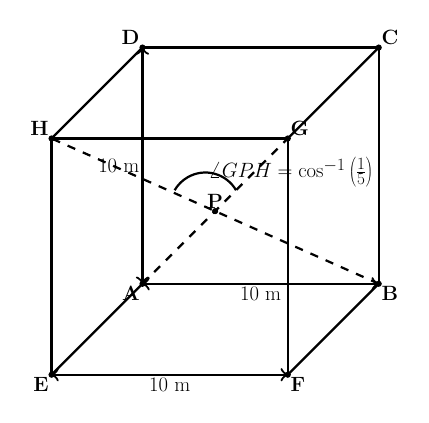
\begin{tikzpicture}[scale=0.3,transform shape]
    \coordinate (A) at (0, 0, 0);
    \coordinate (B) at (10, 0, 0);
    \coordinate (C) at (10, 10, 0);
    \coordinate (D) at (0, 10, 0);
    \coordinate (E) at (0, 0, 10);
    \coordinate (F) at (10, 0, 10);
    \coordinate (G) at (10, 10, 10);
    \coordinate (H) at (0, 10, 10);
    
    \coordinate (P) at (5, 5, 5); 

    \draw[thick] (A) -- (B) -- (C) -- (D) -- cycle;
    \draw[thick] (E) -- (F) -- (G) -- (H) -- cycle; 
    \draw[thick] (A) -- (E);
    \draw[thick] (B) -- (F);
    \draw[thick] (C) -- (G);
    \draw[thick] (D) -- (H);
    
    \draw[dashed, thick] (A) -- (G);
    \draw[dashed, thick] (B) -- (H);

    \foreach \point in {A, B, C, D, E, F, G, H, P} {
        \filldraw[black] (\point) circle (3pt);
    }

    \node at (A) [below left] {\Huge \textbf{A}};
    \node at (B) [below right] {\Huge \textbf{B}};
    \node at (C) [above right] {\Huge \textbf{C}};
    \node at (D) [above left] {\Huge \textbf{D}};
    \node at (E) [below left] {\Huge \textbf{E}};
    \node at (F) [below right] {\Huge \textbf{F}};
    \node at (G) [above right] {\Huge \textbf{G}};
    \node at (H) [above left] {\Huge \textbf{H}};
    \node at (P) [above] {\Huge \textbf{P}};

    \draw[<->, thick] (A) -- (B) node[midway, below] {\Huge 10 m};
    \draw[<->, thick] (A) -- (D) node[midway, left] {\Huge 10 m};
    \draw[<->, thick] (E) -- (F) node[midway, below] {\Huge 10 m};

    \draw[thick] (5.5, 5.5, 4) arc[start angle=30, end angle=150, radius=1.5] node[midway, right] {\Huge $\angle GPH = \cos^{-1}\left(\frac{1}{5}\right)$};

\end{tikzpicture}


\end{center}    
\begin{multicols}{4}
\begin{enumerate}
    \item $5$
    \item $2\sqrt{10}$
    \item $5\sqrt{3}$
    \item $5\sqrt{2}$
\end{enumerate}
\end{multicols}


%\end{enumerate}
%\end{document}




\iffalse
  \title{Assignment}
  \author{EE24BTECH11038}
  \section{mcq-single}
\fi  
\item Let $p_1,p_2,p_3,\cdots,p_{15}$ be points on circle. The number of distinct triangles formed by points $p_i,p_j,p_k$ such that i+j+k$\neq$15, is :\hfill{Aug 2021}
\begin{enumerate}
    \item 12
    \item 419
    \item 443
    \item 455
\end{enumerate}
\bigskip
\item The range of the function,
\begin{align*}
    f\brak{x}=\log_{\sqrt{5}} \left(3+\cos{\brak{\frac{3\pi}{4}+x}}+\cos{\brak{\frac{\pi}{4}+x}}+\cos{\brak{\frac{\pi}{4}-x}}-\cos{\brak{\frac{3\pi}{4}-x}}\right)
\end{align*}
is:\hfill{Aug 2021}
\begin{enumerate}
    \item $\brak{0,\sqrt{5}}$\\
    \item $\sbrak{-2,2}$\\
    \item $\sbrak{\frac{1}{\sqrt{5}},\sqrt{5}}$\\
    \item $\sbrak{0,2}$
\end{enumerate}
\bigskip
\item Let $a_1,a_2,a_3,\cdots,a_{21}$ be an A.P such that $\sum_{n=1}^{20} \frac{1}{a_na_{n+1}}=\frac{4}{9}$. If the sum of this A.P is 189, then $a_6a_{16}$ is equal to :\hfill{Aug 2021}
\begin{enumerate}
    \item 57
    \item 72
    \item 48
    \item 36
\end{enumerate}
\bigskip
\item The function f$\brak{x}$, that satisfies the condition f$\brak{x}$=x+$\int_0^{\frac{\pi}{2}} \sin{x}.\cos{y}f\brak{y}\,dy,$ is :\hfill{Aug 2021}
\begin{enumerate}
    \item x+$\frac{2}{3}\brak{\pi-2}\sin{x}$
    \item  x+$\brak{\pi+2}\sin{x}$
     \item x+$\frac{\pi}{2}\sin{x}$
      \item x+$\brak{\pi-2}\sin{x}$
\end{enumerate}
\bigskip
\item Let $\theta$ be the acute angle between the tangents to the ellipse $\frac{x^2}{9}+\frac{y^2}{1}$=1 and the circle $x^2+y^2=3$ at their point of intersection in the first quadrant then $\tan{\theta}$ is equal to:\hfill{Aug 2021}
\begin{enumerate}
    \item $\frac{5}{2\sqrt{3}}$
    \item $\frac{2}{\sqrt{3}}$
    \item $\frac{4}{\sqrt{3}}$
    \item 2
\end{enumerate}



\iffalse
    \title{2021}
    \author{EE24BTECH11001}
    \section{mcq-single}
\fi
\item 
        Let $P_1, P_2 \dots P_{15}$  be 15 points on a circle. The number of distinct triangles formed by points $P_i, P_j, P_k$ such that 
        $i + j +k \ne 0$ is :
        \hfill{\brak{\textnormal{2021-Sep}}}
        \begin{multicols}{4}
            \begin{enumerate}
                \item 12
                    \columnbreak
                \item 419
                    \columnbreak
                \item 443
                    \columnbreak
                \item 455
            \end{enumerate}
        \end{multicols}

    \item The range of the function 
        \begin{align}
            f\brak{x} = \log_{\sqrt{3}} \brak{3 + \cos \brak{\frac{3\pi}{4} + x} + \cos \brak{\frac{\pi}{4} + x}+ \cos \brak{\frac{\pi}{4} - x} +\cos \brak{\frac{3\pi}{4} - x}}
        \end{align} is :
        \hfill{\brak{\textnormal{2021-Sep}}}
        \begin{multicols}{4}
            \begin{enumerate}
                \item $\brak{0,  \sqrt{5}}$ \columnbreak
                \item $\sbrak{-2, 2}$ \columnbreak
                \item $\sbrak{\frac{1}{\sqrt{5}}, \sqrt{5}}$ \columnbreak
                \item $\sbrak{0, 2}$
            \end{enumerate}
        \end{multicols}


    \item Let $a_1, a_2 \dots a_{21}$ be an AP such that 
        \begin{align}
            \sum_{n = 1} ^{20} \frac{1}{a_{n}a_{n+1}} = \frac{4}{9}
        \end{align}. If the sum of the AP is 189, then $a_{6}a_{16}$ is : 
        \hfill{\brak{\textnormal{2021-Sep}}}
        \begin{enumerate}
                \begin{multicols}{2}
                \item 57 \columnbreak
                \item 72
                \end{multicols}
                \begin{multicols}{2}
                \item 48 \columnbreak
                \item 36
                \end{multicols}
        \end{enumerate}

    \item  The function $f\brak{x}$, that satisfies the condition  
        \begin{align}
            f\brak{x} = x + \int_{0} ^ {\frac{\pi}{2}} \sin x \cos y f\brak{y} \, dy
        \end{align} 
        is : 
        \hfill{\brak{\textnormal{2021-Sep}}}
        \begin{enumerate}
                \begin{multicols}{4}
                \item $x + \frac{2}{3}\brak{\pi - 2}\sin x$ \columnbreak
                \item $x + \brak{\pi + 2}\sin x$ \columnbreak
                \item $x + \frac{\pi}{2}\sin x$ \columnbreak
                \item $x + \brak{\pi - 2}\sin x$
                \end{multicols}
        \end{enumerate}

    \item Let $\theta$ be the acute angle between the tangents to the ellipse 
        \begin{align}
            \frac{x^2}{9} + \frac{y^2}{1} = 1
        \end{align} and the circle 
        \begin{align}
            x^2 + y^2 = 3
        \end{align} at their point of intersection in the first quadrant. Then $\tan \theta$ is equal to :

        \hfill{\brak{\textnormal{2021-Sep}}}
        \begin{enumerate}
            \item $\frac{5}{2\sqrt{2}}$ 
            \item $\frac{2}{\sqrt{3}}$ 
            \item $\frac{4}{\sqrt{3}}$  
            \item $2$
        \end{enumerate}

\iffalse
    \title{2021}
    \author{AI24BTECH11030}
    \section{mcq-single}
\fi

    \item Let $f : \mathbb{R} \rightarrow \mathbb{R}$ be a continuous function. Then
    $\lim_{x \to \frac{\pi}{4}} \frac{\frac{\pi}{4} \int_{2}^{\sec^2 x} f(x) dx}{ x^2 - \frac{\pi^2}{16}}$
    is equal to: \hfill [Aug 2021]
    \begin{multicols}{4}
        \begin{enumerate}
            \item $f(2)$
            \item $2f(2)$
            \item $2f(\sqrt{2})$
            \item $4f(2)$
        \end{enumerate}
    \end{multicols}
    
    \item $\cos^{-1}(\cos(-5)) + \sin^{-1}(\sin(6)) - \tan^{-1}(\tan(12))$ is equal to: \hfill [Aug 2021]
    \begin{multicols}{4}
        \begin{enumerate}
            \item $3\pi - 11$
            \item $4\pi - 9$
            \item $4\pi - 11$
            \item $3\pi + 1$
        \end{enumerate}
    \end{multicols}

    \item Consider the system of linear equations:
    \begin{align*}
        -x + y + 2z &= 0 \\
        3x - ay + 5z &= 1 \\
        2x - 2y - az &= 7
    \end{align*}
    Let $S_1$ be the set of all $a \in \mathbb{R}$ for which the system is inconsistent, and $S_2$ the set of all $a \in \mathbb{R}$ for which the system has infinitely many solutions. If $n(S_1)$ and $n(S_2)$ denote the number of elements in $S_1$ and $S_2$ respectively, then: \hfill [Aug 2021]
    \begin{multicols}{2}
        \begin{enumerate}
            \item $n(S_1) = 2$, $n(S_2) = 2$
            \item $n(S_1) = 1$, $n(S_2) = 0$
            \item $n(S_1) = 2$, $n(S_2) = 0$
            \item $n(S_1) = 0$, $n(S_2) = 2$
        \end{enumerate}
    \end{multicols}
    
    \item Let the acute angle bisector of the planes $x - 2y - 2z + 1 = 0$ and $2x - 3y - 6z + 1 = 0$ be the plane $P$. Which of the following points lies on $P$? \hfill [Aug 2021]
    \begin{multicols}{2}
        \begin{enumerate}
            \item $(3, 1, -\frac{1}{2})$
            \item $(-2, 0, -\frac{1}{2})$
            \item $(0, 2, -4)$
            \item $(4, 0, -2)$
        \end{enumerate}
    \end{multicols}

    \item Which of the following is equivalent to the Boolean expression $p \land \neg q$? \hfill [Aug 2021]
    \begin{multicols}{4}
        \begin{enumerate}
            \item $\neg(q \to p)$
            \item $\neg p \to \neg q$
            \item $\neg(p \to \neg q)$
            \item $\neg(p \to q)$
        \end{enumerate}
    \end{multicols}
    
    \item Two squares are chosen at random on a chessboard. The probability that they have a side in common is: \hfill [Aug 2021]
    \begin{multicols}{4}
        \begin{enumerate}
            \item $\frac{2}{7}$
            \item $\frac{1}{18}$
            \item $\frac{1}{7}$
            \item $\frac{1}{9}$
        \end{enumerate}
    \end{multicols}

    \item If $y = y(x)$ is the solution of the differential equation $x^2 dy + \brak{y - \frac{1}{x}} dx = 0$; $x > 0$ and $y(1) = 1$, then $y\brak{\frac{1}{2}}$ is equal to: \hfill [Aug 2021]
    \begin{multicols}{4}
        \begin{enumerate}
            \item $\frac{3}{2} - \frac{1}{\sqrt{e}}$
            \item $3 + \frac{1}{\sqrt{e}}$
            \item $3 + e$
            \item $3 - e$
        \end{enumerate}
    \end{multicols}

    \item If $n$ is the number of solutions of the equation
    $$
    2\cos x\brak{4\sin\brak{\frac{\pi}{4} + x} \sin\brak{\frac{\pi}{4} - x} -1 } = 1, \: x \in [0, \pi],
    $$
    and $S$ is the sum of all these solutions, then the ordered pair $(n, S)$ is: \hfill [Aug 2021]
    \begin{multicols}{4}
        \begin{enumerate}
            \item $(3, \frac{13\pi}{9})$
            \item $(2, \frac{2\pi}{3})$
            \item $(2, \frac{8\pi}{9})$
            \item $(3, \frac{5\pi}{3})$
        \end{enumerate}
    \end{multicols}

    \item The function $f(x) = x^3 - 6x^2 + ax + b$ is such that $f(2) = f(4) = 0$. Consider two statements:
    \begin{itemize}
        \item[(S1)] There exists $x_1, x_2 \in (2, 4)$, $x_1 < x_2$, such that $f'(x_1) = -1$ and $f'(x_2) = 0$.
        \item[(S2)] There exists $x_3, x_4 \in (2, 4)$, $x_3 < x_4$, such that $f$ is decreasing in $(2, x_4)$, increasing in $(x_4, 4)$ and $2f'(x_3) = \sqrt{3}f(x_4)$.
    \end{itemize}
    Then:  \hfill [Aug 2021]
    \begin{multicols}{2}
        \begin{enumerate}
            \item Both (S1) and (S2) are true
            \item (S1) is false and (S2) is true
            \item Both (S1) and (S2) are false
            \item (S1) is true and (S2) is false
        \end{enumerate}
    \end{multicols}

    \item Let 
    $$
    J_{n,m} = \int_0^\frac{1}{2} \frac{x^n}{x^m-1} dx, \forall n > m \quad \text{and} \quad n, m \in \mathbb{N}.
    $$
    Consider a matrix $A = [a_{ij}]_{3 \times 3}$ where 
    $$
    a_{ij} = \begin{cases} 
    J_{6+i,3} - J_{i+3,3}, & \text{if } i \leq j, \\
    0, & \text{if } i > j.
    \end{cases}
    $$
    Then $\abs{\text{adj} A^{-1}}$ is: \hfill [Aug 2021]
    \begin{multicols}{4}
        \begin{enumerate}
            \item $(15)^2 \times 2^{42}$
            \item $(15)^2 \times 2^{34}$
            \item $(105)^2 \times 2^{38}$
            \item $(105)^2 \times 2^{36}$
        \end{enumerate}
    \end{multicols}

    \item The area enclosed by the curves $y = \abs{\cos x - \sin x}$ and $y = \sin x + \cos x$, and the lines $x = 0$ and $x = \frac{\pi}{2}$ is: \hfill [Aug 2021]
    \begin{multicols}{4}
        \begin{enumerate}
            \item $2\sqrt{2} - 2$
            \item $2 + 2\sqrt{2}$
            \item $4 - 2\sqrt{2}$
            \item $2 + 4\sqrt{2}$
        \end{enumerate}
    \end{multicols}

    \item The distance of the line $3y - 2z - 1 = 0 = 3x - z + 4$ from the point $(2, -1, 6)$ is: \hfill [Aug 2021]
    \begin{multicols}{4}
        \begin{enumerate}
            \item $\sqrt{26}$
            \item $2\sqrt{5}$
            \item $2\sqrt{6}$
            \item $4\sqrt{2}$
        \end{enumerate}
    \end{multicols}

    \item Consider the parabola with vertex $\brak{\frac{1}{2}, \frac{3}{4}}$ and the directrix $y = \frac{1}{2}$. Let $P$ be the point where the parabola meets the line $x = -\frac{1}{2}$. If the normal to the parabola at $P$ intersects the parabola again at the point $Q$, then $(PQ)^2$ is equal to: \hfill [Aug 2021]
    \begin{multicols}{4}
        \begin{enumerate}
            \item $\frac{75}{8}$
            \item $\frac{125}{16}$
            \item $\frac{25}{2}$
            \item $\frac{15}{2}$
        \end{enumerate}
    \end{multicols}

    \item The number of pairs $(a, b)$ of real numbers, such that whenever $\alpha$ is a root of the equation $x^2 + ax + b = 0$, $\alpha^2 - 2$ is also a root of the equation, is: \hfill [Aug 2021]
    \begin{multicols}{4}
        \begin{enumerate}
            \item 6
            \item 2
            \item 4
            \item 8
        \end{enumerate}
    \end{multicols}

    \item Let $S_n = 1\cdot(n-1) + 2\cdot(n-2) + \dots + (n-1)\cdot1$, for $n \geq 4$. The sum 
    $$
    \sum_{n=4}^{\infty} \brak{\frac{2S_n}{n!} - \frac{1}{(n-2)!}}
    $$
    is equal to: \hfill [Aug 2021]
    \begin{multicols}{4}
        \begin{enumerate}
            \item $\frac{e - 1}{3}$
            \item $\frac{e - 2}{6}$
            \item $\frac{e}{3}$
            \item $\frac{e}{6}$
        \end{enumerate}
    \end{multicols}




\end{enumerate}
\subsection*{Integer Value Type Questions}
\begin{enumerate}[label=\thechapter.\arabic*,ref=\thechapter.\theenumi]

\iffalse
\title{2021}
\author{AI24BTECH11031}
\section{integer}
\fi

\item The area bounded by the lines $y = \abs{x - 1} - 2$ is \rule{1cm}{0.15mm}.
\hfill{[Feb 2021]}

\item The number of integral values of $k$ for which the equation
$3\sin x + 4\cos x = k + 1$ has a solution, $k \in \mathbb{R}$ is \rule{1cm}{0.15mm}.
\hfill{[Feb 2021]}

\item Let $m, n \in \mathbb{N}$ and $\gcd(2, n) = 1$. If
$30\binom{30}{0} + 29\binom{30}{1} + \dots + 2\binom{30}{28} + 1\binom{30}{29} = n \cdot 2^m$,
then $n + m = \rule{1cm}{0.15mm}$.
\hfill{[Feb 2021]}

\item If $y = y(x)$ is the solution of the equation $e^{\sin y}\cos y \frac{dy}{dx} + e^{\sin y}\cos x = \cos x$,
$y(0) = 0$; then $1 + y\brak{\frac{\pi}{6}} + \frac{\sqrt{3}}{2} y\brak{\frac{\pi}{3}} + \frac{1}{\sqrt{2}} y\brak{\frac{\pi}{4}}$
is equal to \rule{1cm}{0.15mm}.
\hfill{[Feb 2021]}

\item The number of solutions of the equation $\log_4(x - 1) = \log_2(x - 3)$ is \rule{1cm}{0.15mm}.
\hfill{[Feb 2021]}

\item If $\sqrt{3}(\cos^2 x) = (\sqrt{3} - 1) \cos x + 1$, the number of solutions
of the given equation when $x \in \sbrak{0, \frac{\pi}{2}}$ is \rule{1cm}{0.15mm}.
\hfill{[Feb 2021]}

\item Let $(\lambda, 2, 1)$ be a point on the plane which passes through the point
$(4, -2, 2)$. If the plane is perpendicular to the line joining the points
$(-2, -21, 29)$ and $(-1, -16, 23)$, then $\brak{\frac{\lambda}{11}}^2 - \frac{4\lambda}{11} - 4$
is equal to \rule{1cm}{0.15mm}.
\hfill{[Feb 2021]}

\item The difference between degree and order of a differential equation that
represents the family of curves given by $y^2 = a \brak{x + \frac{\sqrt{a}}{2}}$,
$a > 0$ is \rule{1cm}{0.15mm}.
\hfill{[Feb 2021]}

\item The sum of $162^{th}$ power of the roots of the equation
$x^3 - 2x^2 + 2x - 1 = 0$ is \\
\rule{1cm}{0.15mm}. \hfill{[Feb 2021]}

\item The value of the integral $\int_0^\pi \abs{\sin 2x} dx$ is \rule{1cm}{0.15mm}.
\hfill{[Feb 2021]}

\iffalse
\title{2021}
\author{EE24BTECH11012}
\section{integer}
\fi
%\begin{enumerate}
	\item The number of real roots of the equation $ \brak{x+1}^2 + \abs{x-5} = \frac{27}{4} $ is : \hfill{[Feb 2021]}
	\item The students $S_1, S_2, \dots, S_{10}$ are to be divided into 3 groups A, B and C such that each group has at least one student and the group C has at most 3 students. Then the total number of possibilities of forming such groups is :\hfill{[Feb 2021]}
	\item If $ \emph{a} + \alpha = 1 $, $ \emph{b} + \beta = 2 $ and $af\brak{x} + \alpha\brak{1}{x} = bx + \frac{\beta}{2} $, $ x\neq0 $ then the value of the expression $\frac{\sbrak{f\brak{x} + f\brak{\frac{1}{x}}}}{\brak{x + \frac{1}{x}}}$ :\hfill{[Feb 2021]}
	\item If the variance of 10 natural numbers 1,1,1,\dots,1,\emph{k} is less than 10, then the maximum possible value of \emph{k} is :\hfill{[Feb 2021]}
	\item Let $\lambda$ be an integer. If the shortest distance between the lines $ x - \lambda = 2y - 1 = = -2z $ and $ x = y + 2\lambda = z - \lambda $ is $\frac{\sqrt{7}}{2\sqrt{2}}$, then the value of $\abs{\lambda}$ is :\hfill{[Feb 2021]}
	\item If $ \emph{i} = \sqrt{-1} $. If $ \frac{\brak{-1+\emph{i}\sqrt{3}}^21}{\brak{1-\emph{i}}^24} + \frac{\brak{1+\emph{i}\sqrt{3}}^21}{\brak{1+\emph{i}}^24} = \emph{k}$, and $ \emph{n} = \sbrak{\abs{\emph{k}}}$ be the greatest integral part of $\abs{\emph{k}}$. Then $ \sum_{j=0}^{\emph{n}+5} \brak{j+5}^2 - \sum_{j=0}^{\emph{n+5}} \brak{j+5} $ is equal to : \hfill{[Feb 2021]}
	\item Let a point $\vec{P}$ be such that its distance from the point $\myvec{5,0}$ is thrice the distance of $\vec{P}$ from the point $\myvec{-5,0}$. If the locus of the point $\vec{P}$ is a circle of radius \emph{r}, then $4\emph{r}^2$ is equal to : \hfill{[Feb 2021]}
	\item The maximum value of k for which the sum $ \sum_{i=0}^{k} \comb{10}{i} \comb{15}{k-i} + \sum_{i=0}^{k+1} \comb{12}{i} \comb{13}{k+1-i} $ exists, is equal to : \hfill{[Feb 2021]}

	\item The sum of first four terms of a geometric progression is $\frac{65}{12}$ and the sum of their respective reciprocals is $\frac{65}{18}$. If the product of first three terms of the G.P. is 1, and the third term is $\alpha$ then $2\alpha$ is : \hfill{[Feb 2021]}

	\item If the area of the triangle formed by the positive x-axis, the normal and the tangent to the circle $\brak{x-2}^2 + \brak{y-3}^2 = 25$ at the point $\myvec{5,7}$ is \emph{A}, then 24\emph{A} is equal to :\hfill{[Feb 2021]}
%\end{enumerate}
 %\end{document}

\iffalse
\title{2021}
\author{EE24BTECH11012}
\section{integer}
\fi
%\begin{enumerate}
	\item Let $\vec{a} = \vec{i} - \alpha\vec{j} + \beta\vec{k}$, $\vec{b} = 3\vec{i} + \beta\vec{j} - \alpha\vec{k}$ and $\vec{c} = -\alpha\vec{i} - 2\vec{j} + \vec{k}$, where $\alpha$, $\beta$ are integers. If $\vec{a} \cdot \vec{b} = -1$ and $\vec{b} \cdot \vec{c} = 10$, then $\brak{\vec{a} \times \vec{b}} \cdot \vec{c}$ is equal to :\hfill{[July 2021]}
	\item The distance of the point P$\myvec{3,4,4}$ from the point of intersection of the line joining the points Q$\myvec{3,-4,5}$ and R$\myvec{2,-3,1}$ and the plane $2x+y+z=7$, is equal to :\hfill{[July 2021]}
	\item If the real part of the complex number $ z = \frac{3+2i\cos{\theta}}{1-3i\cos{\theta}}$, $\theta \in \brak{0, \frac{\pi}{2}}$ is zero, then the value of $\sin^{2}{3\theta} + \cos^{2}{\theta}$ is equal to :\hfill{[July 2021]}
	\item Let $\vec{E}$ be an ellipse whose axes are parallel to the co-ordinate axes, having its centre at $\myvec{3,-4}$, one focus at $\myvec{4,-4}$ and one vertex at $\myvec{5,-4}$. If $mx - y = 4$, m>0 is a tangent to the ellipse $\vec{E}$, then the value of 5$m^2$ is equal to :\hfill{[July 2021]}
	\item If $\int_{0}^{\pi} \brak{\sin^{3}{x}}e^{-\sin^{2}{x}} dx = \alpha - \frac{\beta}{e} \int_{0}^{1} \sqrt{t}e^{t} dt$, then $\alpha + \beta$ is equal to :\hfill{[July 2021]}
	\item The number of real roots of the equation $ e^{4x} - e^{3x} - 4e^{2x} - e^{x} + 1 = 0$ is equal to :\hfill{[July 2021]}
	\item Let $ y = y(x) $ be the solution of the differential equation $ dy = e^{\alpha x + y} dx $; $\alpha \in \vec{R}$. If $ y\brak{log\brak{2}} = log\brak{2}$ and $y(0) = log\brak{\frac{1}{2}}$, then the value of $\alpha$ is equal to :\hfill{[July 2021]}
	\item Let $n$ be a non-negative integer. Then the number of divisors of the form "4n+1" of the number $\brak{10}^{10}\brak{11}^{11}\brak{13}^{13}$ is equal to :\hfill{[July 2021]}
	\item Let $A = \cbrak{n \in \vec{N} | n^2 \leq n + 10,000}$, $B = \cbrak{3k+1 | k \in \vec{N}}$ and $C = \cbrak{2k | k \in \vec{N}}$, then the sum of all the elements of the set $ A \cap \brak{ B-C}$ is equal to ;\hfill{[July 2021]}
	\item If $A = \myvec{1&1&1\\0&1&1\\0&0&1}$ and $M = A + A^2 + A^3 + \dots + A^{20} $, then the sum of all the elements of the matrix $M$ is equal to :\hfill{[July 2021]}
%\end{enumerate}
%\end{document}

\iffalse
\title{2021}
\author{EE24Btech11024}
\section{integer}
\fi


\item Let $n\in \mathbb{N}$ and $\sbrak{x}$ denote the greatest integer less than or equal to $x$. If the sum of $\brak{n+1}$ terms $\comb{n}{0}$, $3\cdot\comb{n}{1}$, $5\cdot\comb{n}{2}$, $7\cdot\comb{n}{3} \dots$ is equal to $2^{100}\cdot 101$, then $2\sbrak{\frac{n-1}{2}}$ is equal to \rule{1cm}{0.15mm}.

\hfill{\brak{\text{Jul 2021}}}

\item Consider the function $f\brak{x} = \begin{cases} \frac{P\brak{x}}{\sin\brak{x-2}} & x\neq 2, \\7 & x=2 .\end{cases}$ where $P\brak{x}$ is a polynomial such that ${P^\prime}^\prime\brak{x}$ is always a constant and $P\brak{3}=9$. If $f\brak{x}$ is continuous at $x=2$, then $P\brak{5}$ is equal to \rule{1cm}{0.15mm}.

\hfill{\brak{\text{Jul 2021}}}

\item The equation of a circle is $Re\brak{z^2}+2\brak{Im\brak{z}}^2+2Re\brak{z}=0$, where $z=x+iy$. A line which passes through the centre of the given circle and the vertex of parabola, $x^2-6x-y+13=0$, has y-intercept equal to \rule{1cm}{0.15mm}.

\hfill{\brak{\text{Jul 2021}}}

\item If a rectangle is inscribed in an equilateral triangle of side length $2\sqrt{2}$ as shown in the figure, then the square of the largest area of such a rectangle is \rule{1cm}{0.15mm}.
\\\begin{center}
   \scalebox{0.75}{\begin{tikzpicture}
    \draw (0,0) -- (5,0) -- (2.5,4.33) -- cycle;
    \draw (1,0) -- (1,1.67) -- (4,1.67) -- (4,0) -- cycle;
\end{tikzpicture}}
\end{center}

\hfill{\brak{\text{Jul 2021}}}

\item If $\brak{\vec{a}+3\vec{b}}$ is perpendicular to $\brak{7\vec{a}-5\vec{b}}$ and $\brak{\vec{a}-4\vec{b}}$ is perpendicular to $\brak{7\vec{a}-2\vec{b}}$, then the angle between $\vec{a}$ and $\vec{b}$ \brak{\text{in degrees}} is \rule{1cm}{0.15mm}.

\hfill{\brak{\text{Jul 2021}}}

\item Let a curve $y=f\brak{x}$ pass through the point $\brak{2,\brak{\log_e{2}}^2}$ and have slope $\frac{2y}{x\log_e{x}}$ for all positive real values of $x$. Then the value of $f\brak{e}$ is equal to \rule{1cm}{0.15mm}.

\hfill{\brak{\text{Jul 2021}}}

\item If $a+b+c=1$, $ab+bc+ca=2$ and $abc=3$, then the value of $a^4+b^4+c^4$ is equal to \rule{1cm}{0.15mm}.

\hfill{\brak{\text{Jul 2021}}}

\item A fair coin is tossed $n$-times such that the probability of getting at least one head is at least $0.9$. Then the minimum value of $n$ is \rule{1cm}{0.15mm}. 

\hfill{\brak{\text{Jul 2021}}}

\item If the co-efficient of $x^7$ and $x^8$ in the expansion of $\brak{2+\frac{x}{3}}^n$ are equal, then the value of n is equal to \rule{1cm}{0.15mm}.

\hfill{\brak{\text{Jul 2021}}}

\item If the lines $\frac{x-k}{1}=\frac{y-2}{2}=\frac{z-3}{3}$ and $\frac{x+1}{3}=\frac{y+2}{2}=\frac{z+3}{1}$ are co-planar then, the value of $k$ is \rule{1cm}{0.15mm}.

\hfill{\brak{\text{Jul 2021}}}


\iffalse
\title{2021}
\author{EE24BTECH11012}
\section{integer}
\fi
%\begin{enumerate}
	\item Let $ A = \myvec{2 & -1 & 1 \\ -1 & 2 & -1 \\ 1 & -1 & 2}$ then $det\brak{3Adj\brak{2A^{-1}}}$ is equal to :\hfill{[July 2021]}
	\item If $\myvec{\alpha , \beta}$ is a point on $y^2=6x$, that is closest to $\myvec{3,\frac{3}{2}}$ then find 2 $ \brak{\alpha+\beta} $\hfill{[July 2021]}

	\item Let a function  $g : \sbrak{0,4} \rightarrow \vec{R}$ be defined as
		$$ g(x) = \myvec{ max\brak{t^3-6t^2+9t-3}, & 0 \leq x \leq 3 \\
		                  4 - x, & 3 < x \leq 4 } $$
			then the number of points in the interval \brak{0,4} where g(x) is NOT differentiable is :\hfill{[July 2021]}
		\item The number of solutions of the equation $$\log_{x+1}{\brak{2x^2+7x+5}} + \log_{2x+5}{\brak{x+1}^2} - 4 = 0$$, x $\geq$ 0, is :\hfill{[July 2021]}

	\item Let a curve $ y = y(x)$ be givem by the solutio of the differential equation $$\cos{\brak{\frac{1}{2}\cos^{-1}{e^{-x}}}} dx = \sqrt{e^{2x} - 1} dy $$If it intersects y-axis at $y=-1$ and the intersection point of the curve with the x-axis is $\myvec{\alpha , 0}$, then $e^{\alpha}$ is equal to :\hfill{[July 2021]}
	\item For p $\geq$ 0, a vector $\vec{v_2} = 2\vec{i} + \brak{p+1}\vec{j}$ is obtained by rotating the vector $\vec{v_1} = \sqrt{3}p\vec{i} + \vec{j}$ by an angle $\theta$ about the origin in counter clockwise direction. If $\tan{\theta} = \frac{\alpha\sqrt{3} - 2}{4\sqrt{3} + 3}$, then the value of $\alpha$ is equal to : \hfill{[July 2021]}
	\item Consider a triangle with vertices $\vec{A} \myvec{-2,3}, \vec{B} \myvec{1,9}, \vec{C} \myvec{3,8}$. If a line $\vec{L}$ passing through the circumcentre of the triangle ABC, bisects line BC, and intersects y-axis at point $\myvec{0,\frac{\alpha}{2}}$ then the value of real number $\alpha$ is :\hfill{[July 2021]}
	\item For k $\in \vec{N}$, let $$ \frac{1}{\alpha(\alpha +1)(\alpha +2)\dots(\alpha +20)} = \sum_{k=0}^{20} \frac{A_k}{\alpha + k} $$ where $\alpha>0$.Then the value of 100 $\brak{\frac{A_{14} + A_{15}}{A_{13}}}^2 $ is :\hfill{[July 2021]}
	\item Let $\cbrak{a_{n}}_{n=1}^{\infty}$ be a sequence such that $a_1 = 1$, $a_2 = 1$ and $a_{n+2} = 2a_{n+1} + a_{n}$ for all $n \geq 1$. Then the value of $47 \sum_{n=1}^{\infty} \frac{a_{n}}{2^{3n}}$ is equal to :\hfill{[July 2021]}
	\item If $\lim_{x \to 0} \frac{\alpha xe^{x} - \beta \log\brak{1+x} + \gamma x^2e^{-x}}{x \sin^{2}{x}} = 10 $, $\alpha$, $\beta$, $\gamma \in \vec{R}$, then the value of $\alpha + \beta + \gamma$ is : \hfill{[July 2021]}
%\end{enumerate}
%\end{document}

\iffalse
  \title{Assignment}
  \author{EE24BTECH11038}
  \section{integer}
\fi  
\item Consider a triangle having vertices $\vec{A}\brak{-2,3},\,\vec{B}\brak{1,9},\,\vec{C}\brak{3,8}$. if a line L passing through the circumcentre of triangle ABC, bisects the line BC, and intersects the Y-axis at $\brak{0,\frac{\alpha}{2}}$, then the value of real number $\alpha$ is \hfill{July 2021}
\item Let $\cbrak{a_n}_{n=1}^{\infty}$ be a sequence such that $a_1=1,a_2=1$ and  $a_{n+2}=2a_{n+1}+a_{n}$ for all $n\geq 1$. Then the value of $47\sum_{n=1}^{\infty} \frac{a_n}{2^{3n}}$ is equal to $\cdots$ \hfill{July 2021}
\item The number of solutions of the equation 
\begin{align*}
    \log_{x+1}\left(2x^2+7x+5\right)+\log_{2x+5}\left({x+1}\right)^2-4=0
\end{align*} 
where $x>0$ is \hfill{July 2021}
\item If $\lim_{x\to 0} \frac{\alpha xe^x-\beta\log_{e}^{1+x}+\gamma x^2e^{-x}}{x\sin^2{x}}=10$ ,$\alpha,\,\beta,\,\gamma \in \mathbf{R}$, then the value of $\alpha+\beta+\gamma$ is \hfill{July 2021}
\item For $p>0$, a vector $\vec{v}_2=2\hat{i}+\brak{p+1}\hat{j}$ is obtained by rotating the vector $\vec{v}_1=\sqrt{3}p\hat{i}+\hat{j}$ by an angle $\theta$ about the origin in a counter clock wise direction if $\tan{\theta}=\frac{\alpha \sqrt{3}-2}{4\sqrt{3}+3}$, then the value of $\alpha$ is \hfill{July 2021}
\item Let A=$\cbrak{a_{ij}}$ be a 3 x 3 matrix, where 
\begin{align*}
    a_{ij}=
    \begin{cases}
        \brak{-1}^{j-i} \,\,if \,i<j, \\
        2 \,\, if \,\, i=j, \\
        \brak{-1}^{i+j} \,if\, i>j, 
    \end{cases}
\end{align*}
Then $det\brak{3Adj\brak{2A^{-1}}}$ is equal to  \hfill{July 2021}
\item Let a curve $y=y\brak{x}$ be given by solution of the differential equation 
\begin{align*}
    \cos{\brak{\frac{1}{2}\cos^{-1}{\brak{e^x}}}}\, dx=\sqrt{e^{2x}-1}\,dy
\end{align*}
if it intersects y-axis at y=-1, and the intersection point of the curve with x-axis is $\brak{\alpha,0}$, then $e^{\alpha}$ is equal to \hfill{July 2021}
\item Let a function g:$\sbrak{0,4}\rightarrow \mathbf{R}$ be defined as 
\begin{align*}
    g\brak{x}=
    \begin{cases}
     \max\limits_{\substack{0 \leq t \leq x}} \cbrak{t^3-6t^2+9t-3}, & 0\leq x \leq 3\\
     4-x, & 3 < x\leq 4
    \end{cases}
\end{align*}
then the number of points in the interval $\brak{0,4}$ where $g\brak{x}$ is NOT differentiabe, is  \hfill{July 2021}
\item For k$\in$N, let
\begin{align*}
    \frac{1}{\alpha \brak{\alpha+1} \brak{\alpha+2}\cdots\brak{\alpha+20}}=\sum_{k=0}^{20} \frac{A_k}{\alpha+k}
\end{align*}
where $\alpha>0$ then the value of $100\brak{\frac{A_{14}+A_{15}}{A_{13}}}^2$ is equal to \hfill{July 2021}
\item If the point on the curve $y^2=6x$, nearest to the point $\brak{3,\frac{3}{2}}$ is $\brak{\alpha,\beta}$, then the value of $2\brak{\alpha+\beta}$ is \hfill{July 2021}
   

\iffalse
  \title{Assignment}
  \author{EE24BTECH11038}
  \section{integer}
\fi  

\item Let X be a random variable with distribution.\hfill{Aug 2021}
\begin{table}[!ht]
\centering
\begin{tabular}{ |c|c|c|c|c|c| }
    \hline
    \textbf{X}  & \textbf{-2} & \textbf{-1} & \textbf{3} & \textbf{4} & \textbf{6} \\
    \hline
    $P\left(X=x\right)$ & $\frac{1}{5}$ & $a$ & $\frac{1}{3}$ & $\frac{1}{5}$ & $b$\\   
    \hline
\end{tabular}
\end{table}
If the mean of X is 2.3 and variance of X is $\sigma^2$, then 100$\sigma^2$ is equal to :
\bigskip
\item Let $f\brak{x}=x^6+2x^4+x^3+2x+3$, $x\in \mathbf{R}$. Then the value of natural number n such that  
\begin{align*}
    \lim_{x\to 1}\frac{x^nf\brak{1}-f\brak{x}}{x-1}=44
\end{align*} \hfill{Aug 2021}

\bigskip
\item If for the complex numbers z satisfying $\abs{z-2-2i}\leq 1$, the maximum value of $\abs{3iz+6}$ is attained at a+ib, then the value of a+b is equal to  \hfill{Aug 2021}
\bigskip
\item Let the points of intersections of the lines x-y+1=0,x-2y+3 = 0 and 2x-5y+11=0 are the midpoints of the sides of a triangle ABC. Then the area of triangle ABC is \hfill{Aug 2021}
\bigskip
\item Let f$\brak{x}$ be a polynomial of degree 3 such that$f\brak{k}=-\frac{2}{k}$ for k=2,3,4,5. Then the value of 52-10$f\brak{10}$ is equal to : \hfill{Aug 2021}
\bigskip
\item All the arrangements, with or without meaning, of the word FARMER are written excluding any word that has two R appearing together. The arrangements are listed serially in the alphabetic order as in the English dictionary. Then the serial number of the word FARMER in this list is \hfill{Aug 2021}
\bigskip
\item If the sum of the coefficients in the expansion of $\brak{x+y}^n$ is 4096 then the greatest coefficient in the expansion is \hfill{Aug 2021}
\bigskip
\item Let $\vec{a}= 2\hat{i}-\hat{j} +2\hat{k}$ and $\vec{b}=\hat{i}+ 2\hat{j}-\hat{k}$. Let a vector $\vec{v}$ be in the plane containing $\vec{a} \,\, and\,\, \vec{b}$. If $\vec{v}$ is perpendicular to the vector $3\hat{i}+2\hat{j}-\hat{k}$ and it's projection on $\vec{a}$ is 19 units, then the value of $\abs{2\vec{v}}^2$ is  \hfill{Aug 2021}
\bigskip
\item  Let $\sbrak{t}$ denote the greatest integer $\leq$t. The number of points where the function 
\begin{align*}
    f\brak{x}=\sbrak{x}\abs{x^2-1}+\sin{\brak{\frac{\pi}{\sbrak{x}+3}}}-\sbrak{x+1}, x\in\brak{-2,2}
\end{align*}
is not continuous is.\hfill{Aug 2021}
\bigskip
\item A man starts walking from the point $\vec{P}\brak{-3,4}$ touches the x-axis at R, and then turns to reach at the point $\vec{Q}\brak{0,2}$. The man is walking at a constant speed. If the man reaches the point Q in the minimum time, then $50\brak{\brak{PR}^2+\brak{RQ}^2}$ is equal to \hfill{Aug 2021}


\iffalse
    \title{2021}
    \author{EE24BTECH11001}
    \section{integer}
\fi
\item Let X be the random variable with distribution : 
        \begin{figure}
            \centering
            \begin{tabular}[12pt]{ |c| c| c | c | c| c|}
                \hline
                X & -2 & -1 & 3 & 4 & 6\\ 
                \hline
                $\Pr{X = x}$  & $\frac{1}{5}$ & $a$ & $\frac{1}{3}$ & $\frac{1}{5}$ & $b$ \\
                \hline 
            \end{tabular}
        \end{figure}
        If the mean of X is 2.3 and the variance of X is $\sigma ^ 2$ then $100\sigma ^ 2$ is equal to:
        \hfill{\brak{\textnormal{2021-Sep}}}\\

    \item Let 
        \begin{align}
            f\brak{x} = x^6 + 2x^4 + x^3 + 2x + 3, x \in \textbf{R}. 
        \end{align}
        Then the natural number $n$ for which $lim_{x \to 1} \frac{x^{n}f\brak{1} - f\brak{x}}{x - 1} = 44$ is :
        \hfill{\brak{\textnormal{2021-Sep}}}\\


    \item If for the complex number z satisfying $\abs{z - 2 -2i} \le 1$, the maximum value of $\abs{3iz + 6}$ is attained at $a + ib$, then $a + b$ is equal to
        \hfill{\brak{\textnormal{2021-Sep}}}\\


    \item[24.] 4. Let the points of intersections of the lines $x - y + 1 = 0, x -  2y + 3 = 0$ and $2x - 5y + 11 = 0$ are the mid points
        of the sides of a triangle ABC. Then the area of the triangle ABC is :
        \hfill{\brak{\textnormal{2021-Sep}}}\\


    \item Let $f\brak{x}$  be a polynomial of degree 3 such that $f\brak{k} = -\frac{2}{k}$ for $k = 2, 3, 4, 5$. Then the value of
        $53 - 10f\brak{10}$ is :
        \hfill{\brak{\textnormal{2021-Sep}}}\\


    \item All of the arrangements, with or without meaning, of the word FARMER ae written excluding any word that has two R appering together . The arrangements
        are listed serially in the alphabetic order as in the English dictionary. Then the serial number of the word FARMER in this list is:
        \hfill{\brak{\textnormal{2021-Sep}}}\\


    \item If the sum of the coefficients in the expansion of $\brak{x + y}^n$ is 4096, then the greatest coefficient in the expansion is :
        \hfill{\brak{\textnormal{2021-Sep}}}\\


    \item If $\vec{a} = 2\vec{i} - \vec{j} + 2\vec{k}$ and $\vec{b} = \vec{i} + 2\vec{j} - 1\vec{k}$. Let a vector $\vec{v}$ be in the plane containing
        $\vec{a}$ and $\vec{b}$. If $\vec{v}$ is perpendicular to the vector $3\vec{i} + 2\vec{j} - \vec{k}$ and its projection on $\vec{a}$ is 19 units, 
        then $\norm{2\vec{v}}^2$ is equl to :
        \hfill{\brak{\textnormal{2021-Sep}}}\\


    \item Let $\sbrak{t}$ denote the greatest integer $ \le t $. The number of points where the function
        \begin{align}
            f\brak{x} = \sbrak{x} \abs{x^2 - 1} + \sin \brak{\frac{\pi}{\sbrak{x} + 3}} - \sbrak{x + 1}, x \in \brak{-2, 2} 
        \end{align}
        is not continuous is :
        \hfill{\brak{\textnormal{2021-Sep}}}\\


    \item A man starts walking from the point $P\brak{-3,4}$, touches the $x$-axis at R, and then turns to reach at the point $Q\brak{0, 2}$. The man is walking at a constant
        speed. If the man reaches the point $Q$ in the minimum time, then $50\brak{\brak{PR}^2 + \brak{RQ}^2}$
        \hfill{\brak{\textnormal{2021-Sep}}}
            \begin{center}
            \resizebox{0.5\textwidth}{!}{
            \begin{tikzpicture}[scale = 2]
                \draw[black, thick, domain=-1:-3, samples=100] 
                plot ({\x}, {(-2)*\x - 2}); 
                \draw[black, thick, domain=-3:0, samples=100] 
                plot ({\x}, {2 - 0.6667 *(\x)}); 
                \draw[black, thick, domain=-1:0, samples=100] 
                plot ({\x}, {2 + 2 *(\x)}); 
                \draw[->] (-3, 0) -- (3, 0) node[right] {$x$}; 
                \draw[->] (0, -3) -- (0, 3) node[above] {$y$};	
                \fill[black] (-3, 4) circle (1pt) node[left] {\small $P\brak{-3,4}$};
                \fill[black] (0, 2) circle (1pt) node[right] {\small $Q\brak{0, 2}$};
                \fill[black] (-1, 0) circle (1pt) node[below left] {\small $R\brak{-1, 0}$};		
            \end{tikzpicture}
            }
            \end{center}



\end{enumerate}

\chapter{2022}
\subsection*{MCQs with a Single Correct Answer}
\begin{enumerate}[label=\thechapter.\arabic*,ref=\thechapter.\theenumi]

\iffalse
  \title{Assignment}
  \author{ee24btech11030}
  \section{mcq-single}
\fi

%   \begin{enumerate}
\item  If\\
    
    $$ \sum_{k=1}^{31} \binom{31}{k} \binom{31}{k-1} - \sum_{k=1}^{30} \binom{30}{k} \binom{30}{k-1} = \frac{\alpha \cdot (60!)}{(30!) \cdot (31!)} $$\\ where $\alpha$ $\in$ R, then the value of 16$\alpha$ is equal to \hfill{[JUN 2022]}
    \begin{multicols}{4}
    \begin{enumerate}
        \item 1411
        \item 1320
        \item 1615
        \item 1855
    \end{enumerate}
    \end{multicols}
    \bigskip
    \item Let a function f : N $\rightarrow$ N be defined by\\
    f(x) = $\left[\begin{array}{ll}2n& , n = 2,4,6,8,\cdots\\ n - 1 & , n = 3,7,11,15,\cdots\\\frac{n + 1}{2}  &, n = 1,5,9,13,\cdots \end{array}\right.$\\
    then, f is \hfill{[JUN 2022]}
    \begin{enumerate}
        \item One-one but not onto
        \item Onto but not one-one
        \item Neither one-one nor onto
        \item One-one and onto
    \end{enumerate} 
    \bigskip
    \item If the system of linear equations\\
    2x + 3y - z = -2\\
    x + y + z = 4\\
    x - y + $|\lambda|$z = 4$\lambda$ - 4\\
    where $\lambda$$\in$ R, has no solution, then \\\hfill{[JUN 2022]}
    \begin{multicols}{4}
    \begin{enumerate}
        \item $\lambda = 7$
        \item $\lambda = -7$
        \item $\lambda = 8$
        \item $\lambda^2 = 1$
    \end{enumerate} 
    \end{multicols}
    \bigskip
    \item Let A be a matrix of order 3 $\times$ 3 and det (A) = 2. Then det (det (A) adj (5 adj (A3))) is equal to  \hfill{[JUN 2022]}
    \begin{multicols}{2}
    \begin{enumerate}
        \item $512\times 10^6$
        \item $256\times 10^6$
        \item $1024\times 10^6$
        \item $256\times 10^{11}$
    \end{enumerate} 
    \end{multicols}
    \bigskip
    \item he total number of 5-digit numbers, formed by using the digits 1, 2, 3, 5, 6, 7 without repetition, which are multiple of 6, is \hfill{[JUN 2022]}
    \begin{multicols}{4}
    \begin{enumerate}
        \item 36
        \item 48
        \item 60
        \item 72
    \end{enumerate} 
    \end{multicols}
    \bigskip
    \item Let $A_1, A_2, A_3, \cdots $ be an increasing geometric progression of positive real numbers. If $A_1A_3A_5A_7 = \frac{1}{1296}$ and $A_2 + A_4 = \frac{7}{36}$ then, the value of $A_6 + A_8 + A_{10}$ is equal to\hfill{[JUN 2022]} 
    \begin{multicols}{4}
    \begin{enumerate}
        \item $33$
        \item $37$
        \item $43$
        \item $47$
    \end{enumerate} 
    \end{multicols}
    \bigskip
    \item Let [t] denote the greatest integer less than or equal to t. Then, the value of the integral $\int_{0}^{1}[-8x^{2} + 6x - 1] dx$ is equal to \hfill{[JUN 2022]}
    \begin{multicols}{4}
    \begin{enumerate}
        \item $-1$
        \item $\frac{-5}{4}$
        \item $\frac{\sqrt{17} - 13}{8}$
        \item $\frac{\sqrt{17} - 16}{8}$
    \end{enumerate} 
    \end{multicols}
    \bigskip
    \item Let f: $R \rightarrow R$ be defined as\\
    f(x) = $\left[\begin{array}{ll}0& ,  x<0 \\ ae^{x} - 1 & ,  0 \leq x < 1 \\b & , x = 1\\ 
    b - 1 &, 1 < x < 2\\-c &, x \geq 2 \end{array}\right.$\\Where a, b, c $\in$  R and [t] denotes greatest integer less than or equal to t. Then, which of the following statements is true? \hfill{[JUN 2022]}
    \begin{enumerate}
        \item There exists a, b, c $\in$  R  such that f is continuous on $\in$  R .
        \item If f is discontinuous at exactly one point, then a + b + c = 1
        \item If f is discontinuous at exactly one point, then a + b + c $\neq$ 1
        \item f is discontinuous at atleast two points, for any values of a, b and c
    \end{enumerate}
    \bigskip
    \item The area of the region\\
    $\left\{(x,y) : y^2 \leq 8x , y \geq \sqrt{2}x , x \geq 1 \right\}$
    is \hfill{[JUN 2022]}
    \begin{multicols}{4}
    \begin{enumerate}
        \item $\frac{13\sqrt{2}}{6}$
        \item $\frac{11\sqrt{2}}{6}$
        \item $\frac{5\sqrt{2}}{6}$
        \item $\frac{19\sqrt{2}}{6}$
    \end{enumerate} 
    \end{multicols}
    \bigskip
    \item Let the solution curve y = y(x) of the differential equation 
    $\left[\frac{x}{\sqrt{x^2 - y^2}} + e^{\frac{y}{x}}\right]x\frac{dy}{dx} = x + \left[\frac{x}{\sqrt{x^2 - y^2}} + e^{\frac{y}{x}}\right]y$
    pass through the points (1, 0) and $(2\alpha, \alpha)$, $\alpha > 0$. Then $\alpha$ is equal to \hfill{[JUN 2022]}
    \begin{multicols}{2}
    \begin{enumerate}
        \item $\frac{1}{2}exp(\frac{\pi}{6} + \sqrt{e} - 1)$\\
        \item $\frac{1}{2}exp(\frac{\pi}{3} + \sqrt{e} - 1)$
        \item $exp(\frac{\pi}{6} + \sqrt{e} + 1)$\\
        \item $2 exp(\frac{\pi}{3} + \sqrt{e} - 1)$
    \end{enumerate} 
    \end{multicols}
    \bigskip
    \item Let y = y(x) be the solution of the differential equation $x(1-x^2)\frac{dy}{dx} + 3x^2y - y - 4x^3 = 0$ , x$>$1 with y(2) = -2. Then y(3) is equal to \hfill{[JUN 2022]}
    \begin{multicols}{4}
    \begin{enumerate}
        \item -18
        \item -12
        \item -6
        \item -3
    \end{enumerate}
    \end{multicols}
    \bigskip
    \item The number of real solutions of $x^7 + 5x^3 + 3x + 1 = 0$ is equal to \hfill{[JUN 2022]}
    \begin{multicols}{4}
    \begin{enumerate}
        \item 0
        \item 1
        \item 3
        \item 5
    \end{enumerate} 
    \end{multicols}
    \bigskip
    \item Let the eccentricity of the hyperbola\\H : $\frac{x^2}{a^2} + \frac{y^2}{b^2} = 1\\$be $\frac{\sqrt{5}}{2}$ and length of its latus rectum be $6\sqrt{2}$, If $y = 2x + c$ is a tangent to the hyperbola H. then the value of $c^2$ is equal to \hfill{[JUN 2022]}
    \begin{multicols}{4}
    \begin{enumerate}
        \item 18
        \item 20
        \item 24
        \item 32
    \end{enumerate} 
    \end{multicols}
    \bigskip
    \item If the tangents drawn at the points $\vec{O}\myvec{0,0}$ and $\vec{P}\myvec{1 + \sqrt{5}, 2}$ on the circle $x^2 + y^2 - 2x - 4y = 0$ intersect at the point Q, then the area of the triangle OPQ is equal to \hfill{[JUN 2022]}
    \begin{multicols}{4}
    \begin{enumerate}
        \item $\frac{3 + \sqrt{5}}{2}$
        \item $\frac{4 + 2\sqrt{5}}{2}$
        \item $\frac{5 + 3\sqrt{5}}{2}$
        \item $\frac{7 + 3\sqrt{5}}{2}$
    \end{enumerate} 
    \end{multicols}
    \bigskip
    \item If two distinct points Q, R lie on the line of intersection of the planes $-x + 2y - z = 0$ and $3x - 5y + 2z = 0$ and PQ = PR = $\sqrt{18}$ where the point P is (1, -2, 3), then the area of the triangle PQR is equal to \hfill{[JUN 2022]}
    \begin{multicols}{4}
    \begin{enumerate}
        \item $\frac{2}{3}\sqrt{38}$
        \item $\frac{4}{3}\sqrt{38}$
        \item $\frac{8}{3}\sqrt{38}$
        \item $\sqrt{\frac{152}{3}}$
    \end{enumerate} 
    \end{multicols}
    \bigskip
%   \end{enumerate}

\iffalse
  \title{Assignment}
  \author{ee24btech11030}
  \section{mcq-single}
\fi

%   \begin{enumerate}
\item A biased die is marked with numbers 2, 4, 8, 16, 32, 32 on its faces and the probability of getting a face with mark n is $\frac{1}{n}$. If the die is thrown thrice, then the probability, that the sum of the numbers obtained is 48, is :  \\ \hfill{[JUN 2022]}
    \begin{multicols}{4}
    \begin{enumerate}
        \item $\frac{7}{2^{11}}$
        \item $\frac{7}{2^{12}}$
        \item $\frac{3}{2^{10}}$
        \item $\frac{13}{2^{12}}$
    \end{enumerate}
    \end{multicols}
    \bigskip
    \item The negation of the Boolean expression $((\sim q) \land p) \implies ((\sim p) \lor q)$ is logically equivalent to :  \\\hfill{[JUN 2022]}
    \begin{multicols}{4}
    \begin{enumerate}
        \item $p \implies q$
        \item $q \implies p$
        \item $\sim (p \implies q)$
        \item $\sim (q \implies p)$
    \end{enumerate} 
    \end{multicols}
    \bigskip
    \item If the line $y = 4 + kx$, k $>$ 0, is the tangent to the parabola $y = x - x^2$ at the point $\vec{P}$ and $\vec{V}$ is the vertex of the parabola, then the slope of the line through $\vec{P}$ and $\vec{V}$ is :  \\\hfill{[JUN 2022]}
    \begin{multicols}{4}
    \begin{enumerate}
        \item $\frac{3}{2}$
        \item $\frac{26}{9}$
        \item $\frac{5}{2}$
        \item $\frac{23}{6}$
    \end{enumerate}
    \end{multicols}
    \bigskip
    \item The value of $tan^{-1}{\left(\frac{\cos{\frac{15\pi}{4}} - 1}{\sin{\frac{\pi}{4}}}\right)}$ is equal to: \\\hfill{[JUN 2022]}
    \begin{multicols}{4}
    \begin{enumerate}
        \item $\frac{-\pi}{4}$
        \item $\frac{-\pi}{8}$
        \item $\frac{-5\pi}{12}$
        \item $\frac{-4\pi}{9}$
    \end{enumerate} 
    \end{multicols}
    \bigskip
    \item  The line $y = x + 1$ meets the ellipse $\frac{x^2}{4} + \frac{y^2}{2} = 1$ at two points $\vec{P}$ and $\vec{Q}$. If r is the radius of the circle with PQ as diameter then $(3r)^2$ is equal to : \\\hfill{[JUN 2022]}
    \begin{multicols}{4}
    \begin{enumerate}
        \item 20
        \item 12
        \item 11
        \item 8
    \end{enumerate} 
    \end{multicols}
%   \end{enumerate}

\iffalse
  \title{Assignment}
  \author{ee24btech11030}
  \section{integer}
\fi

%   \begin{enumerate}
\item Let A = $\begin{pmatrix} 2 & -2 \\ 1 & -1 \end{pmatrix}$ and  B = $\begin{pmatrix} -1 & 2 \\ -1 & 2 \end{pmatrix}$\\
    Then the number of elements in the set {(n, m) : n, m $\in$ { 1, 2,$\cdots$, 10} and $nA^n + mB^m = I$} is \underline{\hspace{1cm}}.\hfill{[JUN 2022]}
    \bigskip
    
    \item Let $f(x) = [2x^2 + 1]$ and 
    $g(x) = \begin{cases} 
    2x - 3 & , x < 0 \\ 
    2x + 3 & , x \geq 0 
    \end{cases}$, where  [t] is the greatest integer $\leq t$. Then, in the open interval $(-1, 1)$, the number of points where $f(g(x))$ is discontinuous is equal to \underline{\hspace{1cm}}.\hfill{[JUN 2022]}
    \bigskip
    
    \item The value of b $>$ 3 for which $12\int_{3}^{b}\frac{1}{(x^2 - 1)(x^2 - 4)} \,dx = \ln{(\frac{49}{40})}$, is equal to \underline{\hspace{1cm}}.\hfill{[JUN 2022]}
    \bigskip
    
    \item If the sum of the co-efficients of all the positive even powers of x in the binomial expansion of $\left(2x^3 + \frac{3}{x}\right)^{10}$ is $5^{10} - {\beta}3^9$ then $\beta$ equal to \underline{\hspace{1cm}}\hfill{[JUN 2022]}
    \bigskip
    
    \item If the mean deviation about the mean of the numbers 1, 2, 3, $\cdots$, n, where n is odd, is $\frac{5(n+1)}{n}$, then n is equal to \underline{\hspace{1cm}}.\hfill{[JUN 2022]}
    \bigskip
    
    \item $\overset{\rightarrow}{b} = \hat{i} + \hat{j} + \lambda\hat{k}$ , $\lambda \in R$ . If $\overset{\rightarrow}{b}$ is a vector such that $\overset{\rightarrow}{a} \times \overset{\rightarrow}{b}$ = $13\hat{i} - 1\hat{j} - 4\lambda\hat{k}$ and $\overset{\rightarrow}{a} \cdot \overset{\rightarrow}{b} + 21 = 0$, then $(\overset{\rightarrow}{b} - \overset{\rightarrow}{a}) \cdot (\hat{k} - \hat{j}) + (\overset{\rightarrow}{b} + \overset{\rightarrow}{a}) \cdot (\hat{i} - \hat{k})$ \underline{\hspace{1cm}}. \hfill{[JUN 2022]}
    \bigskip
    
    \item The total number of three-digit numbers, with one digit repeated exactly two times, is \underline{\hspace{1cm}}. \hfill{[JUN 2022]}
    \bigskip
    
    \item Let f(x) = $|(x - 1)(x^2 - 2x - 3)| + x - 3$, x $\in$ R. If m and M are, respectively the number of points of local minimum and local maximum of f in the interval (0, 4), then m + M is equal to \underline{\hspace{1cm}}. \\\\\hfill{[JUN 2022]}
    \bigskip
    
    \item Let the eccentricity of the hyperbola $\frac{x^2}{a^2} - \frac{y^2}{b^2} = 1$ be $\frac{5}{4}$. If the equation of the normal at the point $(\frac{8}{\sqrt{5}},\frac{12}{5})$ on the hyperbola is $8\sqrt{5}x + \beta y = \lambda$, then $\lambda - \beta$ is equal to \underline{\hspace{1cm}}. \hfill{[JUN 2022]}
    \bigskip
    
    \item Let $l_1$ be the line in xy-plane with x and y intercepts $\frac{1}{8}$ and $\frac{1}{4\sqrt{2}}$ respectively and $l_2$ be the line in zx-plane with x and z intercepts $\frac{-1}{8}$ and $\frac{-1}{6\sqrt{3}}$ respectively. If d is the shortest distance between the line $l_1$ and $l_2$, then $d^{-2}$ is equal to \underline{\hspace{1cm}}. \\\\\hfill{[JUN 2022]}
%   \end{enumerate}



\end{enumerate}

\chapter{2023}
\subsection*{MCQs with a Single Correct Answer}
\begin{enumerate}[label=\thechapter.\arabic*,ref=\thechapter.\theenumi]

\iffalse
  \title{2023-02/01/2023-shift-2}
  \author{AI24BTECH11004}
  \section{mcq-single}
\fi
\item The sum 
            \begin{align*}
	       \sum_{n=1}^\infty \frac{2n^2+3n+4}{(2n)!}
            \end{align*}
	is equal to :
	\hfill{[Jan 2023]}
	       \begin{enumerate}
		       \item $\frac{11e}{2}+\frac{7}{2e}$
		       \item $\frac{13e}{4}+\frac{5}{4e}-4$
		       \item $\frac{11e}{2}+\frac{7}{2e}-4$
		       \item $\frac{13e}{4}+\frac{5}{4e}$
        	\end{enumerate}	
	\item Let 
             \begin{align*}  
		S=\cbrak{x\in R: 0<x<1 and 2\tan ^{-1}\brak{\frac{1-x}{1+x}}=\cos ^{-1}\brak{\frac{1-x^2}{1+x^2}}}.
              \end{align*}
	 If $n\brak{S}$ denotes the number of elements in $S$ then :
	\hfill{[Jan 2023]}               
               \begin{enumerate}
			       \item $n\brak{S}=2$ and only one element in $S$ is less than $\frac{1}{2}$
                                \item $n\brak{S}=2$ and only one element in $S$ is less than $\frac{1}{2}$
				\item $n\brak{S}=2$ and only one element in $S$ is less than $\frac{1}{2}$ 
                                \item $n\brak{S}=0$
	       \end{enumerate}	
       \item Let $\overrightarrow{a}=2\hat{i}-7\hat{j}+5\hat{k}$, $\overrightarrow{b}=\hat{i}+\hat{k}$ and $\overrightarrow{c}=\hat{i}+2\hat{j}-3\hat{k}$ be three given vectors. If $\overrightarrow{r}$ is a vector such that $\overrightarrow{r}$x$\overrightarrow{a}=\overrightarrow{c}$x$\overrightarrow{a}$ and $\overrightarrow{r}.\overrightarrow{b}=0$, then $\abs{\overrightarrow{r}}$ is equal to :
       	\hfill{[Jan 2023]}
		\begin{enumerate}
			\item $\frac{11}{7}\sqrt{2}$
			\item $\frac{11}{7}$
			\item $\frac{11}{5}\sqrt{2}$
			\item $\frac{\sqrt{914}}{7}$
		\end{enumerate}
	\item If $A=\frac{1}{2}\myvec{1&\sqrt{3}\\-\sqrt{3}&1}$, then :
		\hfill{[Jan 2023]}
		\begin{enumerate}
			\item $A^{30}-A^{25}=2I$
			\item $A^{30}+A^{25}+A=I$
			\item $A^{30}+A^{25}-A=I$
	                \item $A^{30}=A^{25}$
        	\end{enumerate}
	\item Two sice are thrown independently. Let $A$ be the event that the number appeared on the $1^{st}$ die is less than the number appeared on the $2^{nd}$ die, $B$ be the event that the number appeared on the number appeared on the $1^{st}$ die is even and that on the second die is odd, and $C$ be the event that the number appeared on $i^{st}$ die is odd and that on the $2^{nd}$ is even. Then
		\hfill{[Jan 2023]}
		\begin{enumerate}
			\item the number of favourable cases of the event $\brak{A \cup B}\cap C$ is $6$
			\item $A$ and $B$ are mutually exchusive 
			\item The number of favourabel cases of the events $A,B$ and $C$ are $15,6$ and $6$ respectively 
			\item $B$ and $C$ are independent
        	\end{enumerate}	
	\item Which of the following statements is a tautology ?
		\hfill{[Jan 2023]}
		\begin{enumerate}
			\item $p \rightarrow \brak{p\wedge \brak{p \rightarrow q}}$
			\item $\brak{p\wedge q}\rightarrow \brak{\neg\brak{p}\rightarrow q}$
			\item $\brak{p\wedge \brak {p \rightarrow q}}\rightarrow \neg q$
			\item $p \lor \brak {p \wedge q}$
        	\end{enumerate}
	\item The number of integral values of $k$, for which one root of the equation 
              \begin{align*}
		x^2-8x+k=0
              \end{align*}
		      lies in the interval $(2,3)$, is:
		      	\hfill{[Jan 2023]}
		\begin{enumerate}
			\item $2$
			\item $0$
			\item $1$
			\item $3$
        	\end{enumerate}
	\item Let $f:R-{0,1} \rightarrow R$ be a function such that 
             \begin{align*}
		f\brak{x}+f\brak{\frac{1}{1-x}}=1+x.
             \end{align*}
		Then $f\brak{2}$ is equal to :
			\hfill{[Jan 2023]}
		\begin{enumerate}
			\item $\frac{9}{2}$
                        \item $\frac{9}{4}$
                        \item $\frac{7}{4}$
                        \item $\frac{7}{3}$
        	\end{enumerate}	
	\item  Let the plane $P$ pass through the intersection of the planes $2x+3y-z=2$ and $x+2y+3z=6$, and be perpendicular to the plan $2x+y-z+1=0$. If $d$ is the distance of $P$ from the point $\brak{-7,1,1}$, then $d_2$ is equal to:
		\hfill{[Jan 2023]}
		\begin{enumerate}
			\item $\frac{250}{83}$
			\item $\frac{15}{53}$
			\item $\frac{25}{83}$
			\item $\frac{250}{82}$
        	\end{enumerate}	
	\item Let $a, b$ be two real numbers such that $ab<0$. If the complex number $\frac{1+ai}{b+i}$ is of unit modulus and $a+ib $ lies on the circle $\abs{z-1}=\abs{2z}$, then a possible value of $\frac{1+\abs{a}}{4b}$, where \sbrak{t} is greatest inter function, is : 
	\hfill{[Jan 2023]}
                \begin{enumerate}
			\item $\frac{-1}{2}$
			\item $-1$
			\item $1$
			\item $\frac{1}{2}$
        	\end{enumerate}		
	\item The sum of the abosolute maximum and minimum values of the function 
             \begin{align*}
		f\brak{x} =\abs{x^2-5x+6}-3x+2
             \end{align*}
		in the interval $\sbrak{-1,3}$ is equal to:
			\hfill{[Jan 2023]}
		\begin{enumerate}
			\item $10$
			\item $12$
			\item $13$
			\item $24$
        	\end{enumerate}	
	\item Let $P\brak{S}$ denote the power set of $S =\cbrak{1,2,3,\ldots,10}$. Define the relations $R_1$ and $R_2$ on $P\brak{S}$ as $AR_1B$ if $\brak {A \cap B^c}\cup \brak{B\cap A^c}=\phi$ adn $AR_2B$ if $A\cup B^c=B\cup A^c$, $\forall$ A,B $\in$ P\brak{S}. Then :
		\hfill{[Jan 2023]}
		\begin{enumerate}
			\item both $R_1$ and $R_2$ are equivalence relations
			\item only $R_1$ is an equivalence realtion
			\item only $R_2$ is an euevalence realtaion
			\item both $R_1$ and $R_2$ are not equivalence relations
        	\end{enumerate}	
	\item The area of the region given by $\cbrak{\brak{x,y}:xy \leq 8, 1 \leq y \leq x^2 } is :$
		\hfill{[Jan 2023]}
		\begin{enumerate}
			\item $8 \log^{2}_e-\frac{13}{3}$
			\item $16 \log^{2}_e-\frac{14}{3}$
			\item $8 \log^{2}_e+\frac{7}{6}$
			\item $16 \log^{2}_e+\frac{7}{3}$
        	\end{enumerate}	
	\item Let $\alpha x=exp\brak{x^\beta y^\gamma}$ be the solution of the differential equation 
             \begin{align*}
		2x^2ydy-\brak{1-xy^2}dx=0,
             \end{align*}
	 $x>0$, $y\brak{2}$=$\sqrt{\log_e^2}$. Then $\alpha + \beta - \gamma$ equals :
	 	\hfill{[Jan 2023]}
		\begin{enumerate}
			\item $1$
			\item $-1$
			\item $0$
			\item $3$
        	\end{enumerate}
	\item The value of the integral 
             \begin{align*}
		\int_\frac{-\pi}{4}^\frac{\pi}{4}\frac{x+\frac{\pi}{4}}{2-\cos 2x}dx
             \end{align*}
	     is :
	     	\hfill{[Jan 2023]}
		\begin{enumerate}
			\item $\frac{\pi^2}{6}$
			\item $\frac{\pi^2}{12\sqrt{3}}$
	         	\item $\frac{\pi^2}{3\sqrt{3}}$
                 	\item $\frac{\pi^2}{6\sqrt{3}}$
	\end{enumerate}	




\end{enumerate}

\chapter{2024}
\subsection*{MCQs with a Single Correct Answer}
\begin{enumerate}[label=\thechapter.\arabic*,ref=\thechapter.\theenumi]

\iffalse
    \title{2024}
    \author{EE24BTECH11011}
    \section{mcq-single}
\fi 
\item Let $\vec{OA} = \vec{a} , \vec{OB} = 12\vec{a} + 4\vec{b} \text{ and } \vec{OC} = \vec{b}$ , where $\vec{O}$ is the origin.If $S$ is the parallelogram with adjacent sides $\vec{OA}$ and $\vec{OC}$ , then $\frac{\text{area of the quadrilateral }OABC}{\text{area of }S}$ is equal to \hfill[2024-Jan]
\begin{multicols}{2}
\begin{enumerate}
\item $8$
\item $7$
\item $6$
\item $10$
\end{enumerate}
\end{multicols}
\item Let a unit vector $\vec{u} = x\hat{i}+y\hat{j}+z\hat{k}$ makes angles $\frac{\pi}{2} \frac{\pi}{3} \text{ and } \frac{2\pi}{3}$ with the vectors $\frac{1}{\sqrt{2}}\hat{i}+\frac{1}{\sqrt{2}}\hat{k} , \frac{1}{\sqrt{2}}\hat{j}+\frac{1}{\sqrt{2}}\hat{k} \text{ and } \frac{1}{\sqrt{2}}\hat{i}+\frac{1}{\sqrt{2}}\hat{j}$ respectively.If $\vec{v} = \frac{1}{\sqrt{2}}\hat{i}+\frac{1}{\sqrt{2}}\hat{j}+\frac{1}{\sqrt{2}}\hat{k}$ then $\abs{\vec{u} - \vec{v}}^2 $ is equal to \hfill[2024-Jan]
\begin{multicols}{2}
\begin{enumerate}
\item $9$\\
\item $\frac{5}{2}$
\item $7$\\
\item $\frac{11}{2}$
\end{enumerate}
\end{multicols}
\item The function $f\brak{x} = 2x + 3\brak{x}^{\frac{2}{3}} , x \in \mathbb{R} $ has \hfill[2024-Jan]
	\begin{enumerate}
		\item exactly one point of local minima and no point of local laxima
		\item exactly one point of local maxima and exactly one point of local minima
		\item exactly one point of local maxima and no point of local minima
		\item exactly two points of local maxima and exactly one point of local minima\\
	\end{enumerate}
\item If each term of a geometric peogression $a_1 , a_2 , a_3 ,\dots $ with $a_1 = \frac{1}{8}$ and $a_2 \neq a_1 $ is the arithmetic mean of the next two terms and $S_n = a_1 + a_2 + \dots + a_n$ then $S_{20} - S_{18}$ is equal to \hfill[2024-Jan]
	\begin{multicols}{2}
		\begin{enumerate}
			\item $2^{18}$
			\item $-2^{18}$
			\item $2^{15}$
			\item $-2^{15}$
		\end{enumerate}
	\end{multicols}
	\item If $\log_e a , \log_e b , log_e c $ are in A.P and $log_e{a} - \log_e{2b} , \log_e{2b} - \log_e{3c} , \log_e{3c} - \log_e{a}$ are also in an A.P then $a \colon b \colon c$ is equal to \hfill[2024-Jan]
	\begin{enumerate}
		\item $16 \colon 4 \colon 1$
		\item $6 \colon 3 \colon 2$
		\item $25 \colon 10 \colon 4$
		\item $9 \colon 6 \colon 4$\\
	\end{enumerate}
\item Let $\vec{A} \brak{ 3 , 2 ,3} , \vec{Q}\brak{4 , 6 ,2} \text{ and } \vec{R}\brak{ 7 , 3 ,2}$ be the vertices of $\triangle {PQR}$.Then the angle $\angle{QPR}$ is \hfill[2024-Jan]
	\begin{enumerate}
		\item $\cos ^{-1}\brak{\frac{1}{18}}$
		\item $\frac{\pi}{3}$
		\item $\frac{\pi}{6}$
		\item $\cos^{-1}\brak{\frac{7}{18}}$
	\end{enumerate}
\item Number of ways of arranging $8$ identical books into $4$ identical shelves where any number of shelves may remain empty is equal to \hfill[2024-Jan]
	\begin{multicols}{2}
		\begin{enumerate}
			\item $16$
			\item $18$
			\item $15$
			\item $12$
		\end{enumerate}
	\end{multicols}
\item The distance of the point $\brak{ 2 , 3 }$ from the line $2x - 3y + 28 =0 $ measured parallel to the line $\sqrt{3}x - y + 1 = 0$ is equal to \hfill[2024-Jan]
	\begin{multicols}{2}
		\begin{enumerate}
			\item $ 4 + 6\sqrt{3}$
			\item $ 3 + 4\sqrt{2}$
			\item $6\sqrt{3}$
			\item $4\sqrt{2}$
		\end{enumerate}
	\end{multicols}
\item Let $ y = log_e \brak{\frac{1 - x^2}{1 + x^2}} , -1 < x < 1$ . Then at $x = \frac{1}{2}$, then the value off $225\brak{y^\prime - y^{\prime\prime}}$ is equal to \hfill[2024-Jan]
	\begin{multicols}{2}
		\begin{enumerate}
			\item $736$
			\item $746$
			\item $732$
			\item $742$
		\end{enumerate}
	\end{multicols}
	\item If 
	\begin{align}
		\int \frac{ \sin^{\frac{3}{2}}x + \cos^{\frac{3}{2}}x}{\sqrt{ \sin^3x \cos^3 x \sin \brak{x - \theta}}} dx = A \sqrt{\cos\theta \tan x - \sin \theta} + B \sqrt{ \cos \theta - \sin \theta \cot x} + C 
	\end{align}
	where $C$ is the integration constant, then $AB$ is equal to \hfill[2024-Jan]
	\begin{multicols}{2}
		\begin{enumerate}
			\item $4 \cosec\brak{2\theta}$
			\item $4 \sec{\theta}$
			\item $2 \sec{\theta}$
			\item $8 \cosec\brak{2\theta}$
		\end{enumerate}
	\end{multicols}
\item If $\mathbf{R}$ is the smallest equivalence relation on the set $\cbrak{ 1,2 ,3 ,4}$ such that $\cbrak{\brak{1,2},\brak{1,3}} \subset \mathbf{R}$, then the number of elements in $\mathbf{R}$ is \hfill[2024-Jan]
	\begin{multicols}{2}
		\begin{enumerate}
			\item $12$
			\item $15$\\
			\item $8$
			\item $10$
		\end{enumerate}
	\end{multicols}
\item Let $x = \frac{m}{n} \brak{ m , n \text{ are co-prime natural numbers}}$ be a solution of the equation $\cos \brak{2\sin^{-1}x}=\frac{1}{9}$ and let $\alpha,\beta \brak{\alpha > \beta}$ be the roots of the equation $mx^2 - nx - m + n=0$.Then the point $\brak{\alpha,\beta}$ lies on the line \hfill[2024-Jan]
	\begin{enumerate}
		\item $5x + 8y = 9$
		\item $3x - 3y = -2$
		\item $5x - 8y = -9$
		\item $3x + 2y = 2$
	\end{enumerate}
\item The sum of the solutions $x \in \mathbb{R}$ of the equation 
	\begin{align}
		\frac{3\cos{2x}+\cos^3{2x}}{\cos^{6x}-\sin^3{6x}} = x^3 - x^2 + 6
	\end{align}
	is \hfill[2024-Jan]
	\begin{multicols}{2}
		\begin{enumerate}
			\item $-1$
			\item $1$
			\item $3$
			\item $0$
		\end{enumerate}
	\end{multicols}
	\item Let $\vec{A} = \myvec{ 2 & 1 & 2 \\ 6 & 2 & 11 \\ 3 & 3 & 2} \text{ and } \vec{P} = \myvec{ 1 & 2 & 0 \\ 5 & 0 & 2 \\ 7 & 1 & 5} $. The sum of the prime factors of $\abs{\vec{P}^{-1}\vec{AP}-2\vec{I}}$ is equal to \hfill[2024-Jan]
	\begin{multicols}{2}
		\begin{enumerate}
			\item $26$
			\item $66$
			\item $23$
			\item $27$
		\end{enumerate}
	\end{multicols}
\item An integer is chosen at random from the integers $ 1 , 2 , 3 ,\dots , 50$. The probability that the chosen integer is a multiple of atleast one of $ 4 , 6 \text{ and } 7$ is \hfill[2024-Jan]
	\begin{enumerate}
		\item $\frac{9}{50}$\\
		\item $\frac{8}{25}$\\
		\item $\frac{21}{50}$\\
		\item $\frac{14}{25}$
	\end{enumerate}

\iffalse
\title{Assignment}
\author{K.AKSHAY TEJA}
\section{mcq-single}
\fi
% Question 1
\item If 3, a, b, x are in A.P, and 2, a-1, b+1 are in G.P. Then arithmetic mean of a, b and c is   \hfill \brak{Jan 2024}

\begin{multicols}{4}
\begin{enumerate}
    \item $11$
    \item $10$
    \item $9$
    \item $13$
\end{enumerate}
\end{multicols}

% Question 2
\item The value of $\int_0^{\frac{\pi}{4}} \frac{xdx}{\sin ^4\brak{2x} + \cos ^4\brak{2x}}$ is equal to  \hfill \brak{Jan 2024}

\begin{multicols}{4}
\begin{enumerate}
    \item $\frac{\pi ^2}{16\sqrt{2}}$
    \item $\frac{\pi ^2}{64}$
    \item $\frac{\pi ^2}{32}$
    \item $\frac{\pi ^2}{8\sqrt{2}}$
\end{enumerate}
\end{multicols}



% Question 3
\item If $A = \begin{bmatrix}\sqrt{2} & 1\\-1 & \sqrt{2}
\end{bmatrix}, B = \begin{bmatrix} 1 & 0\\1 & 1
\end{bmatrix}, C = ABA^T,$ then $\abs{X}$ is equal to  \hfill \brak{Jan 2024}
\begin{multicols}{4}
\begin{enumerate}
    \item $729$ 
    \item $283$ 
    \item $27$ 
    \item $23$ 
\end{enumerate}
\end{multicols}



% Question 4
\item If $3, 7, 11, \ldots, 403 = AP_1\,\, 2, 5, 8, \ldots, 401 = AP_2$ Find sum of common term of $AP_1$ and $AP_2$  \hfill \brak{Jan 2024}

\begin{multicols}{4}
    \begin{enumerate}
        \item 3366
        \item 6699
        \item 9999
        \item 6666
    \end{enumerate}
\end{multicols}

% Question 5
\item $\int_\frac{-\pi}{2}^\frac{\pi}{2} \frac{8\sqrt{2}\cos x}{\brak{1 + e^{\sin x}}\brak{1 + \sin^4x}}dx = a\pi + b\log\brak{3 + 2\sqrt{2}}$ then find a + b.  \hfill \brak{Jan 2024}

\begin{multicols}{4}
\begin{enumerate}
    \item $4$
    \item $6$
    \item $8$
    \item $2$
\end{enumerate}
\end{multicols}


% Question 6
\item If $\brak{t+ 1}\,dx = \brak{2x + \brak{t+ 1}^3}\,dt$ and $x\brak{0} = 2$, then $x\brak{1}$ is equal to  \hfill \brak{Jan 2024}

\begin{multicols}{4}
\begin{enumerate}
    \item $5$
    \item $12$
    \item $6$
    \item $8$
\end{enumerate}
\end{multicols}



% Question 7
\item Five people are distributed in four identical rooms. A room can also contain zero people. Find the number of ways to distribute them. \hfill \brak{Jan 2024}
\begin{multicols}{4}
\begin{enumerate}
    \item $47$
    \item $53$
    \item $43$
    \item $51$
\end{enumerate}
\end{multicols}


% Question 8
\item $5f\brak{x} + 4f\brak{\frac{1}{x}} = x^2 -4$ and $y = 9f\brak{x}x^2$. If $y$ is a strictly increasing function, find the interval of $x$.  \hfill \brak{Jan 2024}
\begin{multicols}{2}
\begin{enumerate}
    \item $\brak{ -\infty, \frac{-1}{\sqrt{5}} } \cup \brak{ \frac{-1}{\sqrt{5}}, 0 }$
    \item $\brak{-\frac{-1}{\sqrt{5}},0} \cup \brak{0, \frac{-1}{\sqrt{5}}}$
    \item $\brak{0, \frac{-1}{\sqrt{5}}} \cup \brak{\frac{-1}{\sqrt{5}},\infty}$
    \item $\brak{-\sqrt{\frac{2}{5}}, 0} \cup \brak{\sqrt{\frac{2}{5}}, \infty}$
\end{enumerate}
\end{multicols}


% Question 9
\item If the hyperbola $x^2 - y^2 \cosec^2 \theta = 5$ and the ellipse $x^2 \cosec^2 \theta + y^2 = 5$ has eccentricities $e_H$ and $e_e$ respectively, and $e_H =  \sqrt{7}{e_e}$, then $\theta$ is equal to:  \hfill \brak{Jan 2024}

\begin{multicols}{4}
\begin{enumerate}
    \item $\frac{\pi}{3}$
    \item $\frac{\pi}{6}$
    \item $\frac{\pi}{2}$
    \item $\frac{\pi}{4}$
\end{enumerate}
\end{multicols}

% Question 10
\item A bag contains 8 balls \brak{black and white}. If four balls are chosen without replacement and 2 white \brak{W} and 2 black \brak{B} balls are found, then the probability that the number of white and black balls are the same in the bag is equal to: \hfill \brak{Jan 2024}


\begin{multicols}{4}
\begin{enumerate}
    \item $\frac{1}{7}$
    \item $\frac{2}{7}$
    \item $\frac{3}{5}$
    \item $\frac{1}{2}$
\end{enumerate}
\end{multicols}


% Question 11
\item If two circles $x^2 + y^2 = 4$ and $x^2 + y^2 - 4\lambda x + 9 = 0$ intersect at two distinct points, then find the range of $\lambda$.  \hfill \brak{Jan 2024}
\begin{multicols}{2}
\begin{enumerate}
    \item $\brak{ -\infty, -\frac{13}{2}} \cup \brak{ -\frac{13}{2}, \infty}$
    \item $\brak{ -\infty, -\frac{13}{8}} \cup \brak{ -\frac{13}{8}, \infty}$
    \item $\sbrak{-\frac{13}{8},\frac{13}{8}}$
    \item $\lambda \in \brak{\frac{3}{2},\infty}$
\end{enumerate}
\end{multicols}

% Question 12
\item If $S = \{x \in R : 3\brak{\sqrt{3} + \sqrt{2}}^x + \brak{\sqrt{3} - \sqrt{2}}^x = \frac{10}{3} \}$, then the number of elements in set $S$ is  \hfill \brak{Jan 2024}

\begin{multicols}{4}
\begin{enumerate}
    \item Zero
    \item $1$
    \item $2$
    \item $3$
\end{enumerate}
\end{multicols}




% Question 13
\item $f(x) = \begin{cases} 
e^x, & x < 0 \\
\ln x, & x > 0 
\end{cases} g(x) = \begin{cases} 
e^x, & x < 0 \\
x, & x > 0 
\end{cases}$ The $gof: A \to R$ is   \hfill \brak{Jan 2024}

\begin{multicols}{2}
\begin{enumerate}
    \item Onto but not one-one
    \item Into and many-one
    \item Onto and one-one
    \item Into and one-one
\end{enumerate}
\end{multicols}



% Question 14
\item If $\tan A = \frac{1}{\sqrt{x^2 + x + 1}, \tan B = \frac{\sqrt{x}}{\sqrt{x^2 + x +1}} }$ and $\tan C = \frac{1}{\sqrt{x\brak{x^2 + x +1}}}$, then A + B =  \hfill \brak{Jan 2024}

\begin{multicols}{4}
\begin{enumerate}
    \item $0$ 
    \item $\pi - C$ 
    \item $\frac{\pi}{2} - C$ 
    \item None 
\end{enumerate}
\end{multicols}


% Question 15
\item $\lim_{x \to 0} \frac{\cos^{-1}\brak{1 - \{x\}^2}\sin^{-1}\brak{1 - \{x\}}}{\{x\} - \{x\}^3}$ where \{\} is fractional part function. If L.H.L = L and R.H.L = R, then the correct relation between L and R is \hfill 01-02-2024

\begin{multicols}{4}
\begin{enumerate}
    \item $\sqrt{2}R = 4L$ 
    \item $\sqrt{2}L = 4R$ 
    \item $R = l$ 
    \item $R = 2L$ 
\end{enumerate}
\end{multicols}

%\end{enumerate}
%\end{document}

\iffalse
\title{2024}
\author{AI24BTECH11031}
\section{mcq-single}
\fi

\item For $0 < c < b < a$, let $\brak{a + b - 2c}x^2 + \brak{b + c - 2a}x
    + \brak{c + a - 2b} = 0$ and $\alpha \ne 1$ be one of its roots.
    Then, among the two statements
    \hfill{[Jan 2024]}

    (I) If $\alpha \in \brak{-1, 0}$, then $b$ cannot be the geometric
    mean of $a$ and $c$

    (II) If $\alpha \in \brak{0, 1}$, then $b$ may be the geometric
    mean of $a$ and $c$

    \begin{multicols}{2}
        \begin{enumerate}

            \item Both (I) and (II) are true
            \item Neither (I) nor (II) is true
            \item Only (II) is true
            \item Only (I) is true
        \end{enumerate}
    \end{multicols}

\item Let $a$ be the sum of all coefficients in the expansion of 
    \begin{align*}
    \brak{1 - 2x + 2x^2}^{2023} \brak{3 0 4x^2+2x^3}^{2024}
    \end{align*}
    and $b = \lim\limits_{x \to 0} \brak{\frac{\int_0^x \frac{\log\brak{1+t}}{t^{2024} + 1} dt} {x^2}}$.
    If the equations $cx^2 + dx + e = 0$ and $2bx^2 + ax + 4 = 0$
    have a common root, where $c, d, e \in R$, then $d : c : e$ equals
    \hfill{[Jan 2024]}

    \begin{multicols}{4}
        \begin{enumerate}

            \item $2:1:4$
            \item $4:1:4$
            \item $1:2:4$
            \item $1:1:4$
        \end{enumerate}
    \end{multicols}

\item If the foci of a hyperbola are same as that of the ellipse
    $\frac{x^2}{9} + \frac{y^2}{25} = 1$ and the eccentricity of the
    hyperbola is $\frac{15}{8}$ times the eccentricity of the
    ellipse, then the smaller focal distance of the point
    $\brak{\sqrt{2}, \frac{14}{3} \sqrt{\frac{2}{5}}}$ on the hyperbola,
    is equal to
    \hfill{[Jan 2024]}

    \begin{multicols}{4}
        \begin{enumerate}

            \item $7\sqrt{\frac{2}{5}} - \frac{8}{3}$
            \item $14\sqrt{\frac{2}{5}} - \frac{4}{3}$
            \item $14\sqrt{\frac{2}{5}} - \frac{16}{3}$
            \item $7\sqrt{\frac{2}{5}} + \frac{8}{3}$
        \end{enumerate}
    \end{multicols}

\item If one of the diameters of the circle $x^2 + y^2 - 10x +
    4y + 13 = 0$ is a chord of another circle $C$, whose
    center is the point of intersection of the lines $2x +
    3y = 12$ and $3x - 2y = 5$, then the radius of the
    circle $C$ is
    \hfill{[Jan 2024]}

    \begin{multicols}{4}
        \begin{enumerate}

            \item $\sqrt{20}$
            \item 4
            \item 6
            \item $3\sqrt{2}$
        \end{enumerate}
    \end{multicols}

\item The area of the region
    \begin{align*}
        \cbrak{\brak{x,y}: y^2\le 4x,x<4,\frac{xy\brak{x-1}\brak{x-2}}{\brak{x-3}\brak{x-4}}>0,x\ne3}
    \end{align*}
    is
    \hfill{[Jan 2024]}

    \begin{multicols}{4}
        \begin{enumerate}

            \item $\frac{16}{3}$
            \item $\frac{64}{3}$
            \item $\frac{8}{3}$
            \item $\frac{32}{3}$
        \end{enumerate}
    \end{multicols}

\item If $f\brak{x} = \frac{4x+3}{6x-4}$, $x \ne \frac{2}{3}$ and
    $\brak{fof}\brak{x} = g\brak{x}$, where $g:\mathbb{R} - \cbrak{\frac{2}{3}} \to
    \mathbb{R} - \cbrak{\frac{2}{3}}$ then $\brak{gogog}\brak{4}$ is equal to
    \hfill{[Jan 2024]}

    \begin{multicols}{4}
        \begin{enumerate}

            \item $-\frac{19}{20}$
            \item $\frac{19}{20}$
            \item -4
            \item 4
        \end{enumerate}
    \end{multicols}

\item $\lim\limits_{x \to 0} \frac{e^{2\abs{\sin x}} - 2\abs{\sin x} - 1}{x^2}$
    \hfill{[Jan 2024]}

    \begin{multicols}{4}
        \begin{enumerate}

            \item is equal to -1 
            \item does not exist
            \item is equal to 1 
            \item is equal to 2 
        \end{enumerate}
    \end{multicols}

\item If the system of linear equations
    \begin{align*}
        x - 2y + z = -4 \\
        2x + \alpha y + 3z = 5 \\
        3x - y + \beta z = 3
    \end{align*}
    has infinitely many solutions, then $12\alpha + 13\beta$ is equal to
    \hfill{[Jan 2024]}

    \begin{multicols}{4}
        \begin{enumerate}

            \item 60
            \item 64
            \item 54
            \item 58
        \end{enumerate}
    \end{multicols}

\item The solution curve of the differential equation $y\frac{dx}{dy}
    = x\brak{\log_e x - \log_e y + 1}, x > 0, y > 0$ passing through the point
    $\brak{e, 1}$ is
    \hfill{[Jan 2024]}

    \begin{multicols}{2}
        \begin{enumerate}

            \item $\abs{\log_e \frac{y}{x}} = x$
            \item $\abs{\log_e \frac{y}{x}} = y^2$
            \item $\abs{\log_e \frac{x}{y}} = y$
            \item $\abs{\log_e \frac{x}{y}} = y + 1$
        \end{enumerate}
    \end{multicols}

\item Let $\alpha,\beta,\gamma,\delta \in Z$ and let $A\brak{\alpha,\beta}$,
    $B\brak{1, 0}$, $C\brak{\gamma,\delta}$ and $D\brak{1, 2}$ be the
    vertices of a parallelogram $ABCD$. If $AB = 10$ and the points
    $A$ and $C$ lie on the line $3y = 2x + 1$, then
    $2\brak{\alpha + \beta + \gamma + \delta}$ is equal to
    \hfill{[Jan 2024]}

    \begin{multicols}{4}
        \begin{enumerate}

            \item 10
            \item 5
            \item 12
            \item 8
        \end{enumerate}
    \end{multicols}

\item Let $y = y\brak{x}$ be the solution of the differential equation
    \begin{align*}
        \frac{dy}{dx} = \frac{\brak{\tan x} + y}{\sin x\brak{\sec x - \sin x \tan x}},
        x \in \brak{0, \frac{\pi}{2}}
    \end{align*}
    satisfying the condition $y\brak{\frac{\pi}{4}} = 2$.
    Then $y\brak{\frac{\pi}{3}}$ is
    \hfill{[Jan 2024]}

    \begin{multicols}{2}
        \begin{enumerate}

            \item $\sqrt{3}\brak{2 + \log_e \sqrt{3}}$
            \item $\frac{\sqrt{3}}{2}\brak{2 + \log_e 3}$
            \item $\sqrt{3}\brak{1 + 2 \log_e 3}$
            \item $\sqrt{3}\brak{2 + \log_e 3}$
        \end{enumerate}
    \end{multicols}

\item Let $\overrightarrow{a} = 3\hat{i} + \hat{j} - 2\hat{k}, \overrightarrow{b} = 4\hat{i} + \hat{j} + 7\hat{k}$
    and $\overrightarrow{c} = \hat{i} - 3\hat{j} + 4\hat{k}$ be three vectors. If a
    vector $\overrightarrow{p}$ satisfies $\overrightarrow{p} \times \overrightarrow{b} = \overrightarrow{c} \times \overrightarrow{b}$
    and $\overrightarrow{p} \cdot \overrightarrow{a} = 0$, then $\overrightarrow{p} \cdot \brak{\hat{i} - \hat{j} - \hat{k}}$
    is equal to
    \hfill{[Jan 2024]}

    \begin{multicols}{4}
        \begin{enumerate}

            \item 24
            \item 36
            \item 28
            \item 32
        \end{enumerate}
    \end{multicols}

\item The sum of the series $\frac{1}{1-3\cdot 1^2+1^4}+\frac{2}{1-3\cdot 2^2+2^4}
    +\frac{3}{1-3\cdot 3^2+3^4} + \dots$ upto 10 terms is
    \hfill{[Jan 2024]}

    \begin{multicols}{4}
        \begin{enumerate}

            \item $\frac{45}{109}$
            \item $-\frac{45}{109}$
            \item $\frac{55}{109}$
            \item $-\frac{55}{109}$
        \end{enumerate}
    \end{multicols}

\item The distance of the point $Q\brak{0, 2, -2}$ from the line passing
    through the point $P\brak{5, -4, 3}$ and perpendicular to the lines 
    $\overrightarrow{r} = \brak{-3\hat{i} + 2\hat{k}} + \lambda\brak{2\hat{i} + 3\hat{j} + 5\hat{k}}, \lambda \in \mathbb{R}$
    and $\overrightarrow{r} = \brak{\hat{i} - 2\hat{j} + \hat{k}} + \mu\brak{-\hat{i} + 3\hat{j} + 2\hat{k}}, \mu \in \mathbb{R}$
    is
    \hfill{[Jan 2024]}

    \begin{multicols}{4}
        \begin{enumerate}

            \item $\sqrt{86}$
            \item $\sqrt{20}$
            \item $\sqrt{54}$
            \item $\sqrt{74}$
        \end{enumerate}
    \end{multicols}

\item For $\alpha, \beta, \gamma \ne 0$, if $\sin^{-1}\alpha + \sin^{-1}\beta + \sin^{-1}\gamma = \pi$
    and $\brak{\alpha+\beta+\gamma}\brak{\alpha-\gamma+\beta} = 3\alpha\beta$ then $\gamma$ is
    equal to
    \hfill{[Jan 2024]}

    \begin{multicols}{4}
        \begin{enumerate}

            \item $\frac{\sqrt{3}}{2}$
            \item $\frac{1}{\sqrt{2}}$
            \item $\frac{\sqrt{3} - 1}{2\sqrt{2}}$
            \item $\sqrt{3}$
        \end{enumerate}
    \end{multicols}

\iffalse
  \title{Assignment}
  \author{EE24BTECH11038}
  \section{mcq-single}
\fi 
\item Two marbels are drawn in succession from a box containing 10 red, 30 white, 20 blue and 15 orange marbles, with replacement being made after each drawing. Then the probability, that first drawn marble is red and second drawn marble is white, is \hfill{Jan 2024}
\begin{enumerate}
    \item $\frac{2}{25}$
    \item $\frac{4}{25}$
    \item $\frac{2}{3}$
    \item $\frac{4}{75}$
\end{enumerate}
\bigskip
\item Let $g\brak{x}$ is a linear function and
\begin{align*}
    f\brak{x}=
    \begin{cases}
        g\brak{x}, \,\,\, &x\leq0\\
        \brak{\frac{1+x}{2+x}}^\frac{1}{x} &x>0
    \end{cases}
\end{align*}
is continuous at  x=0 then if $f'\brak{1}=f\brak{-1}$ then the value of $g\brak{3}$ is \hfill{Jan 2024}
\begin{enumerate}
    \item $\frac{1}{3}\log_{e}\frac{4}{9e^{\frac{1}{3}}}$\\
    \item $\frac{1}{3}\log_{e}\brak{\frac{4}{9}}+1$\\
    \item $\log_{e}\brak{\frac{4}{9}}-1$\\
    \item $\log_{e}\frac{4}{9e^{\frac{1}{3}}}$
\end{enumerate}
\bigskip
\item if $f\brak{x}=\begin{vmatrix}
x^3 & 2x^2 + 1 & 1 + 3x \\
3x^2 + 2 & 2x & x^3 + 6 \\
x^3 - x & 4 & x^2 - 2
\end{vmatrix}$ 
for all $x\in \mathbf{R}$, then $2f\brak{0}+f'\brak{0}$ is equal to \hfill{Jan 2024}
\begin{enumerate}
    \item 48
    \item 24
    \item 42
    \item 18
\end{enumerate}
\bigskip
\item Three rotten apples are accidently mixed with fifteen good apples. Assuming the random variable x to be the number of rotten apples in a draw of two apples, the variance of x is  
\begin{enumerate}
    \item $\frac{37}{153}$\\
    \item $\frac{57}{153}$\\
    \item $\frac{47}{153}$\\
    \item $\frac{40}{153}$
\end{enumerate} \hfill{Jan 2024}
\bigskip
\item Let S be the set of positive integral values of a for which $\frac{ax^2+2\brak{a+1}x+9a+4}{x^2-8x+32}<0,\forall x \in\mathbf{R}$ then the number of elements in  S \hfill{Jan 2024}
\begin{enumerate}
    \item 1
    \item 0
    \item $\infty$
    \item 3
\end{enumerate}


\iffalse
\title{April 2024}
\author{EE24Btech11058}
\section{mcq-single}
\fi

%\begin{enumerate}
    \item Let $\int \frac{2 - \tan x}{3+ \tan x} \,dx = \frac{1}{2}\brak{\alpha x + \log_e |\beta \sin x + \gamma \cos x |} + C,$ where $C$ is the constant of integration. Then $\alpha + \frac{\gamma}{\beta}$ is equal to :
    \hfill(April 2024)
    \begin{enumerate}
        \item $1$
        \item $7$
        \item $4$
        \item $3$\\
    \end{enumerate}


    \item A ray of light coming from the point $\vec{P}\brak{1,2}$ gets reflected from $\vec{Q}$ on the $x-axis$ and then passes through the point $\vec{R}\brak{4,3}.$ If the point $\vec{S}\brak{h,k}$ is such that $PQRS$ is a parallelogram, then $hk^2$ is equal to :
    \hfill(April 2024)
    \begin{enumerate}
        \item $80$
        \item $70$
        \item $60$
        \item $90$\\
    \end{enumerate}

    \item $\overrightarrow{OA} = 2 \overrightarrow{a},\overrightarrow{OB} = 6\overrightarrow{a}+ 5\overrightarrow{b}$ and $\overrightarrow{OC} = 3\overrightarrow{b},$ where $O$ is the origin. If the area of the parallelogram with adjacent sides $\overrightarrow{OA}$ and $\overrightarrow{OC}$ is $15sq.units,$ then the area $\brak{in sq.units}$ of the quadrilateral $OABC$ is equal to :
    \hfill(April 2024)
    \begin{enumerate}
        \item $38$
        \item $32$
        \item $40$
        \item $35$\\
    \end{enumerate}

    \item Let $f\brak{x}=x^2+9, g\brak{x}= \frac{x}{x-9}$ and $a=(f \circ g)(10), b= (g \circ f)(3).$ If $e$ and $l$ denote the eccentricity and the length of the latus rectum of the ellipse $\frac{x^2}{a} + \frac{y^2}{b} = 1,$ then $8e^2 + l^2$ is equal to :
    \hfill(April 2024)
    \begin{enumerate}
        \item $16$
        \item $12$
        \item $8$
        \item $6$ \\
    \end{enumerate}


    \item The parabola $y^2=4x$ divides the area of the circle $x^2+y^2=5$ in two parts. The area of the smaller part is equal to :
    \hfill(April 2024)
    \begin{enumerate}
        \item $\frac{1}{3} + \sqrt{5} \sin^{-1} \brak{\frac{2}{\sqrt{5}}}$
        \item $\frac{2}{3} + \sqrt{5} \sin^{-1} \brak{\frac{2}{\sqrt{5}}}$
        \item $\frac{1}{3} + 5 \sin^{-1} \brak{\frac{2}{\sqrt{5}}}$
        \item $\frac{2}{3} + 5 \sin^{-1} \brak{\frac{2}{\sqrt{5}}}$\\
    \end{enumerate}
%\end{enumerate}

  



\iffalse
\title{Assignment}
\author{AI24BTECH11020}
\section{mcq-single}
\fi

%\begin{enumerate}

	\item If the sum of the series $\frac{1}{1.\brak{1+d}}+\frac{1}{\brak{1+d}\brak{1+2d}}+\cdots+\frac{1}{\brak{1+9d}\brak{1+10d}}$ is equal to 5,then 50d is equal to:   \hfill\brak{Apr 2024}
     \begin{enumerate}
     \item $5$ \item $10$ \item $20$ \item $15$
     \end{enumerate}
\item The solution of the differential equation $\brak{x^2+y^2}$d$x$-$5xy$d$y=0$, $y\brak{1}=0,$ is :\hfill\brak{Apr 2024}
      \begin{enumerate}
      \item $\abs{x^2-2y^2}^6=x$
      \item $\abs{x^2-2y^2}^5=x^2$
      \item $\abs{x^2-4y^2}^6=x$
      \item $\abs{x^2-4y^2}^5=x^2$
      \end{enumerate}
\item A variable line $L$ passes through the point $\brak{3,5}$ and intersects the positive coordinate axes at the points $A$ and $B$. The minimum area of the triangle $OAB$, where $O$ is the origin, is: \hfill\brak{Apr 2024}
     \begin{enumerate}
     \item $25$ \item $40$ \item $35$ \item $30$
     \end{enumerate}
\item Let $\alpha ,\beta $ be the roots of the equation $x^2+2\sqrt{2}x-1=0.$ The quadratic equation, whose roots are $\alpha^4+\beta^4$ and $\frac{1}{10}\brak{\alpha^6+\beta^6},$ is : \hfill\brak{Apr 2024}
     \begin{enumerate}
     \item $x^2-180x+9506=0$
     \item $x^2-195x+9506=0$
     \item $x^2-195x+9466=0$
     \item $x^2-190x+9466=0$
     \end{enumerate}
\item Let $f\brak{x}=ax^3+bx^2+cx+41$ be such that $f\brak{1}=40, f'\brak{1}=2 and f''\brak{1}=4.$ Then $a^2+b^2+c^2$ is equal to : \hfill\brak{Apr 2024}
     \begin{enumerate}
     \item $73$ \item $54$ \item $51$ \item $62$
     \end{enumerate}
\item If the domain of the function $f\brak{x}=\sin ^{-1} \brak{\frac{x-1}{2x+3}}$ is $\mathbb{R}-\brak{\alpha,\beta}.$ Then $12\alpha \beta$ is equal to: \hfill\brak{Apr 2024}
     \begin{enumerate}
     \item $36$ \item $32$ \item $24$ \item $40$
     \end{enumerate}
\item Let three vectors $\overrightarrow{a}=\alpha \hat{i}+4\hat{j}+2\hat{k},\overrightarrow{b}=5\hat{i}+3\hat{j}+4\hat{k},\overrightarrow{c}=x\hat{i}+y\hat{j}+z\hat{k}$ form a triangle such that $\overrightarrow{c}=\overrightarrow{a}-\overrightarrow{b}$ and the area of the triangle is $5\sqrt{6}$. If $\alpha$ is a positive real number, then $\abs{\overrightarrow{c}}^2$ is equal to : \hfill\brak{Apr 2024}
     \begin{enumerate}
     \item $16$ \item $10$ \item $14$ \item $12$
     \end{enumerate}
\item Let $\abs{\cos \theta \cos \brak{60^{\circ} -\theta} \cos \brak{60^{\circ} + \theta}} \leq \frac{1}{8}, \theta \in \sbrak{0,2\pi}$. Find the sum of  all $\theta \in \sbrak{0,2\pi}$, where $\cos 3 \theta $ attains its maximum value,is : \hfill\brak{Apr 2024}
     \begin{enumerate}
     \item $18\pi$ \item $9\pi$ \item $6\pi$ \item $15\pi$
     \end{enumerate}
\item The coefficient of $x^{70}$ in $x^2\brak{1+x}^{98}+x^3\brak{1+x}^{97}+x^4\brak{1+x}^{96}+\cdots+x^{54}\brak{1+x}^{46}$ is $\binom{99}{p}-\binom{46}{q}$. Then a possible value of $p + q$ is: \hfill\brak{Apr 2024}
     \begin{enumerate}
     \item $61$ \item $55$ \item $83$ \item $68$
     \end{enumerate}
\item The shortest distance between the lines $\frac{x-3}{4}=\frac{y+7}{-11}=\frac{z-1}{5}$ and $\frac{x-5}{3}=\frac{y-9}{-6}=\frac{z+2}{1}$ is : \hfill\brak{Apr 2024}
     \begin{enumerate}
     \item $\frac{185}{\sqrt{563}}$ 
     \item $\frac{178}{\sqrt{563}}$
     \item $\frac{179}{\sqrt{563}}$
     \item $\frac{187}{\sqrt{563}}$
     \end{enumerate}
\item Let a circle passing through $\brak{2,0}$ have its centre at the point \brak{h,k}. Let $\brak{x_c,y_c}$ be the point of intersection of the lines $3x+5y=1$ and $\brak{2+c}x+5c^2y=1.$ If $\displaystyle \lim_{c \to 1}x_c$ and $\displaystyle \lim_{c \to 1}y_c$, then the equation of the circle is : \hfill\brak{Apr 2024}
     \begin{enumerate}
     \item $25x^2+25y^2-2x+2y-60=0$
     \item $5x^2+5y^2-4x+2y-12=0$
     \item $25x^2+25y^2-20x+2y-60=0$
     \item $5x^2+5y^2-4x-2y-12=0$
     \end{enumerate}
\item Let $\lambda,\mu \in \mathbb{R}.$ If the system of equations\\
	$3x+5y+\lambda z=3$\\
	$7x+11y-9z=2$\\
	$97x+155y+189z=\mu $\\
	has infinitely many solutions, then $\mu +2\lambda$ is equal to : \hfill\brak{Apr 2024}
     \begin{enumerate}
     \item $25$ \item $22$ \item $24$ \item $27$
     \end{enumerate}
\item Let the line $L$ intersect the lines $x-2=-y=z-1,2\brak{x+1}=2\brak{y-1}=z+1$ and be parallel to the line $\frac{x-2}{3}=\frac{y-1}{1}=\frac{z-2}{2}$. Then which of the following points lies on $L$? \hfill\brak{Apr 2024}
     \begin{enumerate}
	\item $\brak{\frac{-1}{3},-1,-1}$
	\item $\brak{\frac{-1}{3},1,-1}$
	\item $\brak{\frac{-1}{3},1,1}$ 
	\item $\brak{\frac{-1}{3},-1,1}$ 
     \end{enumerate}
\item The frequency distribution of the age of students in a class of $40$ students is given below.
	\begin{table}[h]
\centering
\begin{tabular}{|c|c|c|c|c|c|c|}
\hline
Age           & 15  & 16  & 17  & 18  & 19  & 20  \\ \hline
No of Students & 5   & 8   & 5   & 12  & $x$ & $y$ \\ \hline
\end{tabular}
\end{table}
If the mean deviation about the median is $1.25$, then $4x+5y$ is equal to: \hfill\brak{Apr 2024}
     \begin{enumerate}
     \item $47$ \item $43$ \item $46$ \item $44$
     \end{enumerate}
\item The solution curve, of the differential equation $2y \frac{dy}{dx} +3=5\frac{dy}{dx}$, passing through the point $\brak{0,1}$ is a conic, whose vertex lies on the line : \hfill\brak{Apr 2024}
	\begin{enumerate}
     \item $2x+3y=9$ \item $2x+3y=6$ \item $2x+3y=-6$ \item $2x+3y=-9$ 
     \end{enumerate}

%\end{enumerate}
 

 

\iffalse
\title{Assignment}
\author{EE24BTECH11047}
\section{mcq-single}
\fi
\item Let the range of the function $f\brak{x}=\frac{1}{2+\sin{3x}+\cos{3x}},x\in\mathbf{R}$ be $\sbrak{a, b}$. If $\alpha$ and $\beta$ are respectively the arithmetic mean and the geometric mean of $a$ and $b$, then $\frac{\alpha}{\beta}$ is equal to: \hfill(Apr-2024)
\begin{enumerate}
    \item $\pi$
    \item $\sqrt{\pi}$
    \item $2$
    \item $\sqrt{2}$
\end{enumerate}
\item If an unbiased die is rolled thrice, then the probability of getting a greater number in the $i^{th}$ roll than the number obtained in the $\brak{i-1}^{th}$ roll for $i = 2, 3$, is equal to: \hfill(Apr-2024)
\begin{enumerate}
    \item $2/54$
    \item $5/54$
    \item $1/54$
    \item $3/54$
\end{enumerate}
\item Let the foci of a hyperbola H coincide with the foci of the ellipse E:$\frac{\brak{x-1}^2}{100} + \frac{\brak{y-1}^2}{75} = 1$ and the eccentricity of $H$ be the reciprocal of the eccentricity of the ellipse E. If the length of the transverse axis of $H$ is $\alpha$ and the length of its conjugate axis is $\beta$, then $3\alpha^2 + 2\beta^2$ is equal to \hfill(Apr-2024)
\begin{enumerate}
    \item 225
    \item 205
    \item 237
    \item 242
\end{enumerate}
\item Let $\int_0^x\sqrt{1-\brak{y^{\prime}\brak{t}}^2}dt, 0\leq x \leq 3,y\geq 0,y\brak{0}=0.$ Then at $x=2,y^n+y+1$ is equal to \hfill(Apr-2024)
\begin{enumerate}
    \item 2
    \item $\sqrt{2}$
    \item 1/2
    \item 1
\end{enumerate}
\item The sum of the coefficients of $x^{2/3}$ and $x^{-2/5}$ in the binomial expansion of $\brak{x^{2/3}+\frac{1}{2}x^{-2/5}}^9$ is \hfill(Apr-2024)
\begin{enumerate}
    \item $19/4$
    \item $69/16$
    \item $63/16$
    \item $21/4$
\end{enumerate}
\item The value of the integral $\int_{-1}^{2} \log{\brak{x + \sqrt{x^{2}+1}}} dx$ is \hfill(Apr-2024)
\begin{enumerate}
    \item $\sqrt{5}-\sqrt{2}+\log{\brak{\frac{9+4\sqrt{5}}{1+\sqrt{2}}}}$
    \item $\sqrt{2}-\sqrt{5}+\log{\brak{\frac{9+4\sqrt{5}}{1+\sqrt{2}}}}$
    \item $\sqrt{5}-\sqrt{2}+\log{\brak{\frac{7+4\sqrt{5}}{1+\sqrt{2}}}}$
    \item $\sqrt{2}-\sqrt{5}+\log{\brak{\frac{7+4\sqrt{5}}{1+\sqrt{2}}}}$
\end{enumerate}
\item $\lim_{x \to \frac{\pi}{2}} \brak{ \frac{\int_{x^3}^{\brak{ \frac{\pi}{2} }^3} \brak{ \sin \brak{ 2t^{1/3} } + \cos \brak{ t^{1/3} } } \, dt }{\brak{x - \frac{\pi}{2}}^2} }$ is equal to \hfill(Apr-2024)
\begin{enumerate}
    \item $\frac{9\pi^2}{8}$
    \item $\frac{3\pi^2}{2}$
    \item $\frac{11\pi^2}{10}$
    \item $\frac{5\pi^2}{9}$
\end{enumerate}
\item Let $a,ar,ar^2,\cdots$ be an infinite G.P. If $\sum_{n=0}^{\infty}ar^n=57$ and $\sum_{n=0}^{\infty}a^3r^{3n}=9747$, then $a+18r$ is equal to \hfill(Apr-2024)
\begin{enumerate}
	\item 27
	\item 31
	\item 46
	\item 38
\end{enumerate}
\item If $\log_e y = 3\arcsin{x}$, then $\brak{1-x^2}y^{\prime\prime}-xy^{\prime}$ at $x = 1/2$ is equal to: \hfill(Apr-2024)
\begin{enumerate}
    \item $3e^{\pi/2}$
    \item $9e^{\pi/6}$
    \item $9e^{\pi/2}$
    \item $3e^{\pi/6}$
\end{enumerate}
\item $\lim_{x \to 0} \frac{e-\brak{1+2x}^{1/2x}}{x}$ is equal to \hfill(Apr-2024)
\begin{enumerate}
    \item 0
    \item $-2/e$
    \item $e$
    \item $e-e^2$
\end{enumerate}
\item Let $\vec{a} = 2\hat{i} + \alpha\hat{j} + \hat{k}, \vec{b} = -\hat{i} + \hat{k}, \vec{c}=\beta\hat{j}-\hat{k},$ where $\alpha$ and $\beta$ are integers and $\alpha\beta=-6$. Let the values of the ordered pair $\brak{\alpha,\beta}$, for which the area of the parallelogram of diagonals $\vec{a}+\vec{b}$ and $\vec{b}+\vec{c}$ is $\frac{\sqrt{21}}{2}$, be $\brak{\alpha_1,\beta_1}$ and $\brak{\alpha_2,\beta_2}$. Then $\alpha_1^2+\beta_1^2-\alpha_2\beta_2$ is equal to \hfill(Apr-2024)
\begin{enumerate}
    \item $17$
    \item $24$
    \item $19$
    \item $21$
\end{enumerate}
\item Between the following two statements:\\
Statement 1: Let $\vec{a}=\hat{i}+2\hat{j}-3\hat{k}$ and $\vec{b}=2\hat{i}+\hat{j}-\hat{k}$. Then the vector $\vec{r}$ satisfying $\vec{a}\times\vec{r}=\vec{a}\times\vec{b}$ and $\vec{a}\cdot\vec{r}=0$ is of magnitude $\sqrt{10}$.\\
Statement 2: In a triangle ABC, $\cos{2A}+\cos{2B}+\cos{2C}\geq -\frac{3}{2}.$ \hfill(Apr-2024)
\begin{enumerate}
    \item Both Statement 1 and Statement 2 are correct.
    \item Both Statement 1 and Statement 2 are incorrect.
    \item Statement 1 is correct but Statement 2 is incorrect.
    \item Statement 1 is incorrect but Statement 2 is correct.
\end{enumerate}
\item Let $z$ be a complex number such that the real part of $\frac{z-2i}{z+2i}$ is zero. Then, the maximum value of $\abs{z-\brak{6+8i}}$ is equal to \hfill(Apr-2024)
\begin{enumerate}
    \item 10
    \item $\infty$
    \item 8
    \item 12
\end{enumerate}
\item If the variance of the frequency distribution \\
\begin{tabular}{|c|c|c|c|c|c|c|} 
    \hline
        $x$ & c & 2c & 3c & 4c & 5c & 6c \\ 
    \hline
        $f$ & 2 & 1 & 1 & 1 & 1 & 1 \\ 
    \hline
\end{tabular}\\
is 160, then the value of $c\in\mathbf{N}$ is \hfill(Apr-2024)
\begin{enumerate}
    \item 5
    \item 6
    \item 8
    \item 7
\end{enumerate}
\item Let $a, b ;a > b$, be the roots of the equation $x^2 - \sqrt{2}x - \sqrt{3} = 0$. Let $P_n = a^n-b^n$, $n\in\mathbf{N}$. Then $(11\sqrt{3} - 10\sqrt{2})P_{10} + (11\sqrt{2} + 10)P_{11} - 11P_{12}$ is equal to: \hfill(Apr-2024)
\begin{enumerate}
    \item $10\sqrt{2} P_9$
    \item $10\sqrt{3} P_9$
    \item $11\sqrt{2} P_9$
    \item $11\sqrt{3} P_9$
\end{enumerate}


\iffalse
\title{Assignment}
\author{EE24BTECH11035}
\section{mcq-single}
\fi

%\begin{enumerate}

    \item Consider the line $L$ passing through the points $(1, 2, 3)$ and $(2, 3, 5)$. The distance of the point 
    \begin{equation*}
    \left( \frac{11}{3}, \frac{11}{3}, \frac{19}{3} \right)
    \end{equation*}
    from the line $L$ along the line 
    \begin{equation*}
    \frac{3x - 11}{2} = \frac{3y - 11}{1} = \frac{3z - 19}{2}
    \end{equation*}
is equal to:\hfill{(April 2024)}
    \begin{enumerate}
        \item $5$
        \item $4$
        \item $3$
        \item $6$
    \end{enumerate}
    \item Let 
    \begin{equation*}
    B = \begin{bmatrix} 1 & 3 \\ 1 & 5 \end{bmatrix}
    \end{equation*}
    and $A$ be a $2 \times 2$ matrix such that $AB^{-1} = A^{-1}$. If $BCB^{-1} = A$ and 
    \begin{equation*}
    C^4 + \alpha C^2 + \beta I = 0
    \end{equation*}
then $2\beta - \alpha$ is equal to:\hfill{(April 2024)}
    \begin{enumerate}
        \item $8$
        \item $2$
        \item $16$
        \item $10$
    \end{enumerate}
		
\item The area (in square units) of the region enclosed by the ellipse $x^2 + 3y^2 = 18$ in the first quadrant below the line $y = x$ is:\hfill{(April 2024)}
    \begin{enumerate}
        \item ${\sqrt{3}\pi + 1}$
        \item $\sqrt{3}\pi +\frac{3}{4}$
        \item ${\sqrt{3}\pi}$
        \item $\sqrt{3}\pi +\frac{3}{4}$
    \end{enumerate}
\item Two vertices of a triangle $ABC$ are $A(3, -1)$ and $B(2, -3)$, and its orthocenter is $P(1,1)$. If the coordinates of the point $C$ are $(\alpha,\beta)$ and the center of the circle circumscribing the triangle $PAB$ is $(h,k)$, then the value of $(\alpha+\beta) + 2(h+k)$ equals:\hfill{(April 2024)}
 \begin{enumerate}
        \item $81$
        \item $15$
        \item $5$
        \item $51$
    \end{enumerate}
		
    \item The integral
    \begin{equation*}
\int_{\frac{1}{4}}^{\frac{3}{4}} \cos\left( 2 \cot^{-1} \sqrt{\frac{1 - x}{1 + x}} \right) \, dx
\end{equation*}
	is equal to:\hfill{(April 2024)}
    \begin{enumerate}
        \item $1/2$
        \item $1/4$
        \item $-1/4$
        \item $-1/2$
    \end{enumerate}

\iffalse
    \title{2024}
    \author{EE24BTECH11001}
    \section{mcq-single}
\fi

\item 
	    Let a circle C of radius 1 and closer to the origin be such that the lines
        passing through the point $\brak{3, 2}$ and parallel to the coordinate axes touch it.
        Then the shortest distance of the circle from the point $\brak{5, 5}$ is :
		\hfill{\brak{2024-Apr}}
	\begin{multicols}{4}
		\begin{enumerate}
			\item 5
			\columnbreak
        \item $4\sqrt{2}$
			\columnbreak
			\item 4
			\columnbreak
        \item $2\sqrt{2}$
		\end{enumerate}
	\end{multicols}

	\item
        Let a rectangle $ABCD$ of sides 2 and 4 be inscribed in another rectangle $PQRS$
        such that the vertices of the rectangle $ABCD$ lie on the sides og the rectangle $PQRS$.
        Let $a$ and $b$ be the sides of the rectangle $PQRS$ when its area is maximum. Then
        $\brak{a + b}^2$ is equal to :
		\begin{multicols}{4}
		\begin{enumerate}
			\item 80 \columnbreak
			\item 60 \columnbreak
			\item 72 \columnbreak
			\item 64
		\end{enumerate}
	\end{multicols}


\item If
	\begin{align}
        \frac{1}{\sqrt{1} + \sqrt{2}} + \frac{1}{\sqrt{2} + \sqrt{3}} + \dots \frac{1}{\sqrt{99} + \sqrt{100}} = m
	\end{align} and
    \begin{align}
        \frac{1}{1 . 2} + \frac{1}{2 . 3} + \dots \frac{1}{99 . 100} = n
    \end{align} then the point $\brak{m, n}$ lies on the line
		\hfill{\brak{2024-Apr}}
		\begin{enumerate}
            \item $11\brak{x-1} - 100\brak{y-2}$ 
            \item $11\brak{x-2} - 100\brak{y-1}$ 
            \item $11\brak{x-1} - 100y$ 
            \item $11x - 100y$ 
		\end{enumerate}
		
	\item Let $d$ be this distance of the point of intersection of the lines
        \begin{align}
            \frac{x-6}{3} = \frac{y}{2} = \frac{z+1}{1} 
        \end{align} and 
        \begin{align}
            \frac{x-7}{4} = \frac{y-9}{3} = \frac{z-4}{2}
        \end{align} from the point $\brak{7, 8, 9}$. Then $d^2 + 6$ is equal to :
        \hfill{\brak{2024-Apr}}
		\begin{enumerate}
			\begin{multicols}{4}
				\item 72 \columnbreak
				\item 78 \columnbreak
				\item 69 \columnbreak
				\item 75
			\end{multicols}
		\end{enumerate}

	\item Let the line $2x + 3y - k = 0, k > 0$, intersect the x-axis and y-axis at the points 
        $A$ and $B$, respectively. If the equation of the circle having the line segment $AB$ as
        a diameter is $x^2 + 9y^2 = k^2$ is $\frac{m}{n}$, where $m$ and $n$ are coprime, then
        $2m + n$ is equal to :
		\hfill{\brak{2024-Apr}}
		\begin{enumerate}
                \begin{multicols}{4}
			\item 11 \columnbreak 
			\item 10 \columnbreak
			\item 13 \columnbreak
			\item 12  
                \end{multicols}
		\end{enumerate}
	\item
        The coefficients $a, b, c$ in the quadratic equation $ax^2 + bx +c = 0$ are chosen from the 
        set $\{ 1, 2 , 3, 4, 5, 6, 7, 8\}$. The probability of this equation having repeated roots is :
		\hfill{\brak{2024-Apr}}
		\begin{multicols}{4}
		\begin{enumerate}
            \item $\frac{3}{128}$ \columnbreak
            \item $\frac{1}{64}$ \columnbreak
            \item $\frac{1}{128}$ \columnbreak
            \item $\frac{3}{256}$
		\end{enumerate}
	\end{multicols}
\item Suppose $\theta \in \sbrak{0, \frac{\pi}{4}}$ is a solution of $4\cos \theta - 3 \sin \theta = 1$. 
    Then $\cos \theta$ is equal to :
		\hfill{\brak{2024-Apr}}
		\begin{enumerate}
            \item $\frac{4}{\brak{3\sqrt{6} - 2}}$ 
            \item $\frac{6 - \sqrt{6}}{\brak{3\sqrt{6} - 2}}$ 
            \item $\frac{4}{\brak{3\sqrt{6} + 2}}$ 
            \item $\frac{6 + \sqrt{6}}{\brak{3\sqrt{6} + 2}}$ 
		\end{enumerate}
\item
    For the function
	\begin{align}
        f\brak{x} = \sin x + 3x - \frac{2}{\pi}\brak{x^2 + x}, \textnormal{where} x \in \sbrak{0, \frac{\pi}{2}}
	\end{align} 
    Consider the follwing two statements,
    \begin{enumerate}
        \item[1.] $f$ is increasing in $\brak{0, \frac{\pi}{2}}$
        \item[2.] $f'$ is decreasing in $\brak{0, \frac{\pi}{2}}$
    \end{enumerate}
		\hfill{\brak{2024-Apr}}
		\begin{enumerate}
			\item Only 2 is true.
			\item  neither 1 nor 2 is true.
			\item  both 1 and 2 are true.
			\item only 1 is true.
		\end{enumerate}
    \item Let $f\brak{x} = x^5 + 2x^3 + 3x + 1, x \in \mathbb{R},$ and $g\brak{x}$ be a function 
        such that $g\brak{f\brak{x}} = x$ for all $x \in \mathbb{R}$. Then $\frac{g\brak{7}}{g'\brak{7}}$
        is equal to:
		\hfill{\brak{2024-Apr}}
        \begin{multicols}{4}
            
		\begin{enumerate}
			\item 7 \columnbreak
			\item 42 \columnbreak 
			\item 14 \columnbreak
			\item 1
		\end{enumerate}
        \end{multicols}
\item If the system of equations 
		\begin{align}
            11x + y + \lambda z = -5 \\
            2x + 3y + 5z = 3 \\
            8x - 19y - 39z = \mu
		\end{align}, has infinitely many solutions, then $\lambda ^ 4 - \mu$ is equal to :
        \hfill{\brak{2024-Apr}}
		\begin{multicols}{4}
		\begin{enumerate}
			\item 45 \columnbreak
			\item 51 \columnbreak 
			\item 47 \columnbreak
			\item 49
		\end{enumerate}
        \end{multicols}
		\
\item The value of 
    \begin{align}
        \int_{-\pi} ^{\pi} \frac{2y\brak{1 + \sin y}}{1 + \cos ^2 y} \, dy 
    \end{align} is :
		\hfill{\brak{2024-Apr}}
		
	\begin{multicols}{4}
		\begin{enumerate}
            \item $\frac{\pi}{2}$ \columnbreak
            \item $\frac{\pi ^ 2}{2}$ \columnbreak
            \item $\pi ^ 2$ \columnbreak
			\item $2\pi ^2 $
		\end{enumerate}
	\end{multicols}
\item If the line $\frac{2-x}{3} = \frac{3y-2}{4\lambda} = 4-z$ makes right angle with 
    the line $\frac{x+3}{3\mu} = \frac{1-2y}{6} = \frac{5-z}{7}$ the value of $4\lambda + 9\mu$ is :
		\hfill{\brak{2024-Apr}}
		\begin{multicols}{4}
		\begin{enumerate}
			\item 13 \columnbreak
			\item 5 \columnbreak 
			\item 4 \columnbreak
			\item 6
		\end{enumerate}
        \end{multicols}
    \item If $A\brak{1, -1, 2}, B\brak{5, 7, -6}, C\brak{3, 4, -10}$ and $D\brak{-1, -4, -2}$ 
        are the vertices of a quadrilateral $ABCD$, then its area is :
		\hfill{\brak{2024-Apr}}
	\begin{multicols}{4}
		\begin{enumerate}
            \item $12\sqrt{29}$ \columnbreak
            \item $24\sqrt{29}$ \columnbreak
            \item $48\sqrt{7}$ \columnbreak
            \item $24\sqrt{7}$
		\end{enumerate}
	\end{multicols}
\item Let $A$ and $B$ be the two square matrices of order 3 such that $\abs{A} = 3$ 
    and $\abs{B} = 8$. Then\\ 
    $\abs{A^{\top}A\brak{\textnormal{adj}\brak{2A}}^{-1}\brak{\textnormal{adj}\brak{4b}\brak{\textnormal{adj}\brak{AB}^{-1}AA^{\top}}}}$
    is equal to :
		\hfill{\brak{2024-Apr}}
	\begin{multicols}{4}
		\begin{enumerate}
            \item $64$ \columnbreak
            \item $81$ \columnbreak
            \item $108$ \columnbreak
            \item $32$
		\end{enumerate}
	\end{multicols}
\item Let $A = \{ 1, 3, 5, 7, 9\}$ and $B = \{ 2, 4, 5, 7, 8, 10, 12 \}$. Then the total
    number of one-one maps $f : A \rightarrow B$, such that $f\brak{1} + f\brak{3} = 14$ is :
		\hfill{\brak{2024-Apr}}
	\begin{multicols}{4}
		\begin{enumerate}
			\item $120$ \columnbreak
			\item $180$ \columnbreak
			\item $480$ \columnbreak
			\item $240$
		\end{enumerate}
	\end{multicols}

\iffalse
\title{2024}
\author{EE24Btech11024}
\section{mcq-single}
\fi

\item Let $\vec{A}\brak{-1,1}$ and $\vec{B}\brak{2,3}$ be two points and $\vec{P}$ be a variable point above the line $AB$ such that the area of $\Delta PAB$ is 10. If the locus of $\vec{P}$ is $ax+by=15$, then $5a+2b$ is:

\hfill{\brak{\text{Apr 2024}}}
\begin{enumerate}
\begin{multicols}{4}
\item $6$
\item $4$
\item $-\frac{12}{5}$
\item $-\frac{6}{5}$
\end{multicols}
\end{enumerate}

\item Let $\alpha\beta\neq 0$ and $A=\myvec{\beta & \alpha & 3\\\alpha & \alpha & \beta\\-\beta & \alpha & 2\beta}$. If $B=\myvec{3\alpha & -9 & 3\alpha\\-\alpha & 7 & -2\alpha \\ -2\alpha & 5 & -2\beta}$ is the matrix of cofactor elements of $A$, then $\det\brak{AB}$ is equal to:

\hfill{\brak{\text{Apr 2024}}}
\begin{enumerate}
\begin{multicols}{4}
\item $216$
\item $343$
\item $64$
\item $125$
\end{multicols}
\end{enumerate}

\item The value of $m$, $n$ for which the system of linear equations \newline $x+y+z=4$, \newline $2x+5y+5z=17$, \newline $x+2y+mz=n$ \newline has infinitely many solutions satisfy the equation:

\hfill{\brak{\text{Apr 2024}}}
\begin{enumerate}
\begin{multicols}{2}
\item $m^2+n^2-m-n=46$	
\item $m^2+n^2+mn=68$
\item $m^2+n^2+m+n=64$
\item $m^2+n^2-mn=39$
\end{multicols}
\end{enumerate}

\item Let $ABCD$ and $AEFG$ be squares of side $4$ and $2$ units respectively. The point $\vec{E}$ is on the line segment $AB$ and the point $\vec{F}$ is on the diagonal $AC$. Then the radius $r$ of the circle passing through the point $\vec{F}$ and touching the line segments $BC$ and $CD$ satisfies:
\begin{enumerate}
\begin{multicols}{4}
\item $r=1$
\item $r^2-8r+8=0$
\item $2r^2-8r+7=0$
\item $2r^2-4r+1=0$
\end{multicols}
\end{enumerate}

\item Let $\vec{a}=2\hat{i}+5\hat{j}-\hat{k}$, $\vec{b}=2\hat{i}-2\hat{j}+2\hat{k}$ and $\vec{c}$ be three vectors such that $\brak{\vec{c}+\hat{i}}\times\brak{\vec{a}+\vec{b}+\hat{i}}=\vec{a}\times\brak{\vec{c}+\hat{i}}$. If $\vec{a}\cdot\vec{c}=-29$, then $\vec{c}\cdot\brak{-2\hat{i}+\hat{j}+\hat{k}}$ is equal to:

\hfill{\brak{\text{Apr 2024}}}
\begin{enumerate}
\begin{multicols}{4}
\item $15$
\item $12$
\item $5$
\item $10$
\end{multicols}
\end{enumerate}

\iffalse
\title{2024}
\author{EE24BTECH11050-Pothuri Rahul}
\section{mcq-single}
\fi
\item %16
If the line segment joining the points $\brak{5,2}$ and $\brak{2,a}$ subtends an angle $\frac{\pi}{4}$ at the origin, then the absolute value of the product of all possible values of $a$ is :
\begin{enumerate}
\begin{multicols}{4}
\item $4$
\item $2$
\item $6$
\item $8$
\end{multicols}
\end{enumerate}
\item %17
If the shortest distance between the lines $\frac{x - \lambda}{2} = \frac{y - 4}{3} = \frac{z - 3}{4}$ and $\frac{x - 2}{4} = \frac{y - 4}{6} = \frac{z - 7}{8}$ is $\frac{13}{\sqrt{29}}$, then the value of $\lambda$ is :
\begin{enumerate}
\begin{multicols}{4}
\item $-1$
\item $1$
\item $\frac{13}{25}$
\item $ - \frac{13}{25}$
\end{multicols}
\end{enumerate}
\item %18
The number of ways five alphabets can be chosen from the alphabets of the word MATHEMATICS, where the chosen alphabets are not necessarily distinct, is equal to :
\begin{enumerate}
\begin{multicols}{4}
\item $175$
\item $179$
\item $181$
\item $177$
\end{multicols}
\end{enumerate}
\item %19
if $\alpha \neq a, \beta \neq b, \gamma \neq c$ and  
$\abs{\begin{array}{ccc}
\alpha & b & c \\ a & \beta & c \\ a & b & \gamma \end{array}} =0 $, then $\frac{a}{\alpha - a}+\frac{b}{\beta - b}+\frac{\gamma}{\gamma - c}$ is equal to :
\begin{enumerate}
\begin{multicols}{4}
\item $2$
\item $3$
\item $0$
\item $1$
\end{multicols}
\end{enumerate}
\item %20
For $a, b >0$,  let $f\brak{x}= 
\begin{cases}
\frac{\tan{\brak{\brak{a+1}x}}+b\tan{x}}{x} &, x < 0; \\
3 &,  x = 0; \\
\frac{\sqrt{ax+b^2x^2} - \sqrt{ax}}{b\sqrt{a}x\sqrt{x}} &,  x>0;
\end{cases} $ 
be a continuous function at $x=0$. Then $\frac{b}{a}$ is equal to :
\begin{enumerate}
\begin{multicols}{4}
\item $5$
\item $4$
\item $6$
\item $8$
\end{multicols}
\end{enumerate}





\iffalse
\title{2024}
\author{EE24BTECH11050-Pothuri Rahul}
\section{mcq-single}
\fi
\item %21
Let a ray of light passing through the point $\brak{3,10}$ reflects on the line $2x+y=6$ and then reflected ray passes through the point $\brak{7,2}$. If the equation of the incident ray is $ax+by+1=0$, then $a^2+b^2+3ab$ is equal to \underline{\hspace{1cm}}.
\item %22
Let $\alpha \abs{x} = \abs{y} e^{xy - \beta}, \alpha , \beta \in \mathbb{N} $ be the solution of the differential equation $xdy-ydx+xy\brak{xdy+ydx} = 0$, $y\brak{1} = 2 $. Then $\alpha + \beta $ is equal to \underline{\hspace{1cm}}.
\item %23
Let $a,b,c \in \mathbb{N}$ and $a<b<c$. Let the mean, the mean deviation about the mean and the variance of the 5 observations $9,25,a,b,c$ be 18 , 4 and $\frac{136}{5}$, respectively. Then $2a+b-c$ is equal to \underline{\hspace{1cm}}.
\item %24
Let $\vec{S}$ be the focus of the hyperbola $\frac{x^2}{3} - \frac{y^2}{5} = 1$, on the positive x-axis. Let $C$ be the circle its centre at $\vec{A\brak{\sqrt{6},\sqrt{5}}}$ and passing through the points $\vec{S}$. If $\vec{O}$ is the origin and $SAB$ is a diameter of $C$, then the square of the area of the triangle $OSB$ is equal to \underline{\hspace{1cm}}. 
\item %25
Let $A$ be the region enclosed by the parabola $y^2 = 2x$ and the line $x=24$. Then the maximum area of the rectangle inscribed in the region A is: \underline{\hspace{1cm}}.
\item %26
An arithmetic progression is written in the following way 
$
\begin{array}{ccccccc}
& & & 2\\
& & 5 & & 8 & & \\
& 11 &  & 14 & & 17 & \\
20 & & 23 & & 26 & & 29  \\
\_ \_ \_ \_ & \_ \_ \_ \_ & \_ \_ \_ \_ & \_ \_ \_ \_ & \_ \_ \_ \_ & \_ \_ \_ \_ & \_ \_ \_ \_ \\
\_ \_ \_ \_ & \_ \_ \_ \_ & \_ \_ \_ \_ & \_ \_ \_ \_ & \_ \_ \_ \_ & \_ \_ \_ \_ & \_ \_ \_ \_ 
\end{array}
$\\
\\
The sum of all the terms in 10th row is \underline{\hspace{1cm}}.
\item %27
The number of distinct real roots of the equation $\abs{x + 1} \abs{x + 3} - 4\abs{x + 2} + 5 = 0$ is \underline{\hspace{1cm}}.
\item %28
If $\alpha = \lim\limits_{x \to 0^+} \brak{\frac{e^{\sqrt{\tan{x}}} - e^{\sqrt{x}}}{\sqrt{\tan{x}}-\sqrt{x}}}$ and $\beta = \lim\limits_{x \to 0}\brak{1+\sin{x}}^{\frac{1}{2}\cot{x}}$ are the roots of the quadratic equation $ax^2+bx-\sqrt{e} = 0$, then $12 \log_e \brak{a+b}$ is equal to \underline{\hspace{1cm}}. 
\item %29 
If $  \int \frac{1}{\sqrt[5]{\brak{x-1}^4\brak{x+3}^6}} dx = A\brak{\frac{\alpha x -1}{\beta x + 3}}^B + C$, where C is constant of integration, then the value of $\alpha + \beta +20AB$ is \underline{\hspace{1cm}}.
\item %30
let $\vec{P}\brak{\alpha , \beta , \gamma }$ be the image of the point $\vec{Q}\brak{1 , 6, 4}$ in the line $\frac{x}{1} = \frac{y-1}{2} = \frac{z-2}{3}$. Then $2\alpha +\beta +\gamma$ is equal to \underline{\hspace{1cm}}.


\iffalse
\title{06-04-2024}
\author{EE24BTECH11004}
\section{mcq-single}
\fi
\item $I = \int_{0}^{\frac{\pi}{4}} \frac{\cos^2 x \sin^2 x}{\left( \cos^3 x + \sin^3 x \right)^2} \, dx$
\begin{enumerate}
    \item $\frac{1}{6}$
    \item $\frac{1}{3}$
    \item $\frac{1}{2}$
    \item $1$
\end{enumerate}
\item Find the range of $x$ for which $f(x) = x^x \, (x > 0)$ is strictly increasing.
\begin{enumerate}
    \item $ (0, \infty) $
    \item $ \left( 0, \frac{1}{e} \right] $
    \item $ \left[ \frac{1}{C^2}, \infty \right) $
    \item $ \left[ \frac{1}{e}, \infty \right) $
\end{enumerate}
\item Let $A = \{100, 101, 102, \dots, 700\}$. Find the number of numbers in set $A$ which are neither divisible by 3 nor by 4.
\item Given that $\frac{dy}{dx} + 2x \ln{x} \cdot y = 3 \ln{x}$, and $y(1) = 0$, find $y$.
\item Let 
$A_r = \begin{vmatrix}
r & 1 & \frac{n^2}{2} + \alpha \\
2r & 2 & n^2 - \beta \\
3r - 2 & 3 & n(n-1)
\end{vmatrix}$
Find $2A_{10} - A_8$.
\begin{enumerate}
    \item $ 4\alpha + 2\beta $
    \item $ 2n $
    \item $ 0 $
    \item $ 2\alpha + 4\beta $
\end{enumerate}
\item If mean of $20$ observation is$ 10$, $SD = 2$. One of the observation which is $12$ is replaced by$ 8$.
Find the value of new $SD$?
\begin{enumerate}
    \item $ \sqrt{3.96} $
\item $1.8$
\item $ \sqrt{3.8} $
\item $1.93$
\end{enumerate}
\item Let $f : \mathbb{R} \to \mathbb{R}$ be defined by $f(x) = \frac{x^2 - 2x - 15}{x^2 - 4x + 9}$, then $f$ is:
    \begin{enumerate}
        \item one-one onto
        \item many-one onto
        \item many-one into
        \item one-one into
    \end{enumerate}
\item A company has two branches $A$ and $B$. Branch $A$ produces $60\%$ of the total production and the remaining by branch $B$. Branch $A$ produces $80\%$ good quality products, and branch $B$ produces $90\%$ good quality products. A product is randomly selected, and it is found to be of good quality. Let $P$ be the probability that the selected product is from branch $B$. Find the value of $126P$.
\begin{enumerate}
    \item $54$
    \item $52$
    \item $48$
    \item $27$
\end{enumerate}
\item Find the shortest distance between two lines:
$\frac{x - 3}{2} = \frac{y + 15}{-7} = \frac{z - 9}{5}\quad \quad$ and $\frac{x + 1}{2} = \frac{y - 1}{1} = \frac{z-9}{-3}$
\begin{enumerate}
    \item $4 \sqrt{3}$
    \item $8 \sqrt{3}$
    \item $6 \sqrt{3}$
    \item $2 \sqrt{3}$
\end{enumerate}
\item If in the expansion of  $(x + y)^n$, the terms are:
$T_2 = 15, \quad T_3 = 10, \quad T_4 = \frac{10}{3}$ For $n = 5$,  find the value of  $n^3+x^5+243y^5$.
\begin{enumerate}
    \item $ \frac{e^2 + 1}{e} $
    \item $ \frac{e^2 - 1}{e} $
    \item $ \frac{e^2 + 2}{e} $
    \item $ \frac{e^2 - 2}{e} $
\end{enumerate}
\item Let $S = \{1, 2, 3, \dots, 20\}$ be a given set. Relation $R_1$ is defined as $R_1 = \{(x, y) : 2x - 3y = 2\}$ and $R_2$ as $R_2 = \{(x, y) : 4x = 5y\}$, where $x, y \in S$. If $m$ denotes the number of elements required to make $R_1$ symmetric, and $n$ denotes the number of elements to make $R_2$ symmetric,find $m+n$.
\begin{enumerate}
    \item $10$
    \item $12$
    \item $8$
    \item $20$
\end{enumerate}
\item An equilateral triangle of side $12$. A circle is embedded inside the triangle, and a square is embedded inside the circle. If the area and perimeter of the square are $m$ and $n$, respectively, then find $m + n^2$.
\item In an octagon how many triangles are possible so that no side of triangle is side of octagon?
\item A variable line is passing through \brak{4, -9}, slope of line is positive and it make intercepts on
x and y-axis on point A and B. Find the minimum area of triangle OAB.
\item Solve: $\left(1 + x^2 \right) \frac{dy}{dx} + y = e^{\tan^{-1}x}, \, y(1) = 0$. Then $y(0) =$
%\end{enumerate}



\end{enumerate}
\subsection*{Integer Value Type Questions}
\begin{enumerate}[label=\thechapter.\arabic*,ref=\thechapter.\theenumi]

\iffalse
  \title{Assignment}
  \author{EE24BTECH11038}
  \section{integer}
\fi 
\item If the integral 
\begin{align*}
    525\int_{0}^{\frac{\pi}{2}}\sin{2x}\cos^{\frac{11}{2}}{x}\brak{1+\cos^{\frac{5}{2}}{x}}\,dx
\end{align*}
is equal to $\brak{n\sqrt{2}-64}$ then n is equal to \hfill{Jan 2024}
\bigskip
\item Let $S=\brak{-1,\infty}$ and $f:S\rightarrow \mathbf{R}$ defined as 
\begin{align*}
    f\brak{x}=\int_{-1}^{x}\brak{e^{11}-1}^{11}\brak{2t-1}^5\brak{t-3}^{12}\brak{2t-10}^{61}\,dt
\end{align*}
Let p = Sum of square of the values of x, where f$\brak{x}$ attains local maxima on S. and q = Sum of the values of x, where f$\brak{x}$ attains local minima on S. Then, the value of $p^{2}$+2q is \hfill{Jan 2024}
\bigskip
\item The total number of words with or without meaning that can be formed out of the letters of the word `DISTRIBUTION' taken four at a time, 
is equal to,\hfill{Jan 2024}
\bigskip
\item Let Q and R be the feet of perpendiculars from the point $p\brak{a,a,a}$ on the lines x = y, z = 1 and x = -y,z = -1 respectively. If $\angle{QPR}$ is a right angle, then $12a^2$ is equal to \hfill{Jan 2024}
\bigskip
\item In the expansion of 
\begin{align*}
    \brak{1+x}\brak{1-x^2}\brak{1+\frac{3}{x}+\frac{3}{x^2}+\frac{1}{x^3}}^5, x\neq=0
\end{align*}
then the sum of coefficients of $x^3$ and $x^{-13}$ \hfill{Jan 2024}
\bigskip
\item if $\alpha$ denotes the number of solutions of $\abs{1-i}^{x}=2^x$ and $\beta=\brak{\frac{z}{arg\brak{z}}}$ where z$=\frac{\pi}{4}\brak{i+1}^4\brak{\brak{\frac{1-\sqrt{\pi}i}{\sqrt{\pi}+i}}+\brak{\frac{\sqrt{\pi}-1}{1+\sqrt{\pi}i}}},i=\sqrt{-1}$ then the  distance of the point $\brak{\alpha,\beta}$ from the line 4x-3y=7 \hfill{Jan 2024}
\bigskip
\item Let the foci and length of the latus rectum of an ellipse $\frac{x^2}{a^2}+\frac{y^2}{b^2}=1$, a$>$b be $\brak{\pm5,0}$ and $\sqrt{50}$ then the square of eccentrcity of hyperbola $\frac{x^2}{b^2}+\frac{y^2}{a^2b^2}=1$ \hfill{Jan 2024}
\bigskip
\item Let $\vec{a},\vec{b}$ be two vectors such that $\abs{a}=1,\abs{b}=4$ and a.b=2. If $\vec{c}=\brak{2\vec{a}\times\vec{b}}-3\vec{b}$ and the angle between $\vec{b}$ and $\vec{c}$ is $\alpha$ then 192$\sin^2{\alpha}$ \hfill{Jan 2024}
\bigskip
\item Let A = $\cbrak{1, 2, 3, 4}$ and R = $\cbrak{\brak{1, 2}, \brak{2, 3}, \brak{1, 4}}$ be a relation on A. Let  be the equivalence relation on A such that R $\subset$ S and the number of elements in S is n. Then, the minimum value of n is \hfill{Jan 2024}
\bigskip
\item Let f : $\mathbf{R} \rightarrow \mathbf{R}$ be a function defined by f$\brak{x}=\frac{4^x}{4^x+2}$ and 
\begin{align*}
    M=\int_{f\brak{a}}^{f\brak{1-a}} x\sin^{4}\brak{x\brak{1-x}}\,dx\\
    M=\int_{f\brak{a}}^{f\brak{1-a}} \sin^{4}\brak{x\brak{1-x}}\,dx   
\end{align*}
$\alpha M=\beta N$ then the value of $\alpha^2+\beta^2$ is \hfill{Jan 2024}


\iffalse
\title{April 2024}
\author{EE24BTECH11058}
\section{integer}
\fi

%\begin{enumerate}
   \item Let A be a non-singular matrix of order $3$. If $det\brak{3adj\brak{2adj\brak{\brak{det A}A}}} = 3^{-13} . 2^{-10}$ and $det\brak{3adj\brak{2A}}= 2^m.3^n$ , then $|3m + 2n|$ is equal to $ \rule{2cm}{0.15mm}.$ 
   \hfill(April 2024) \\

   \item  The sum of the square of the modulus of the elements in the set $ \{ z=a+ib : a,b \in \textbf{Z},z \in \textbf{C},|z-1| \le 1,\\ |z-5| \le |z-5i| \}$  is $ \rule{2cm}{0.15mm}.$ 
   \hfill(April 2024) \\

   \item Let the centre of a circle, passing through the points $\brak{0,0}, \brak{1,0}$ and touching the circle $x^{2} + y^{2} = 9,$ be $\brak{h,k}$. Then for all possible values of the coordinates of the centre $\brak{h,k} , 4\brak{h^{2} + k^{2}} $ is equal to $\rule{2cm}{0.15mm}$.
   \hfill(April 2024) \\

   \item Let $f:\brak{0,\pi} \rightarrow\textbf{R}$ be a function given by 
   \begin{align*}
   f(x) =
    \begin{cases} 
     \brak{\frac{8}{7}} ^ \frac{\tan 8x}{\tan 7x} & 0 <x<\frac{\pi}{2} \\
      a-8 & x = \frac{\pi}{2}\\
      \brak{1+|\cot x|} ^ {\frac{b}{a} |tanx|} & \frac{\pi}{2} < x <\pi
        \end{cases}
  \end{align*}
  where $a,b \in \textbf{Z}.$ If $f$ is continuous at $x = \frac{\pi}{2},$ then $a^2 + b^2$ is equal to $\rule{2cm}{0.15mm}$.\hfill(April 2024) \\

  \item The remainder when $428 ^{2024}$ is divided by $21$ is $\rule{2cm}{0.15mm}$. 
  \hfill(April 2024) \\

  \item Let $\lim_{n\rightarrow\infty}\brak{\frac{n}{\sqrt{n^{4}+1}}-\frac{2n}{(n^{2}+1)\sqrt{n^{4}+1}}+\frac{n}{\sqrt{n^{4}+16}}-\frac{8n}{(n^{2}+4)\sqrt{n^{4}+16}} +\cdots+\frac{n}{\sqrt{n^{4}+n^{4}}}-\frac{2n\cdot n^{2}}{(n^{2}+n^{2})\sqrt{n^{4}+n^{4}}}}$ be $\frac{\pi}{k},$ using only the principal values of the inverse trigonometric functions.Then $k^2$ is equal to $\rule{2cm}{0.15mm}$.
  \hfill(April 2024)\\
 
  \item If a function $f$ satisfies $f\brak{m+n} = f\brak{m} + f\brak{n}$ for all $m,n \in \textbf{N}$ and $f\brak{1} = 1,$ then the largest natural number $\lambda$ such that $\sum_{k=1}^{2022} f\brak{\lambda + k} \le \brak{2022} ^ 2$ is equal to $\rule{2cm}{0.15mm}$.
  \hfill(April 2024) \\

  \item Let the set of all positive values of $\lambda,$ for which the point of local minimum of the function $\brak{1+x\brak{{\lambda} ^2 - x^2}}$ satisfies $\frac{x^2 + x+2}{x^2+5x+6} < 0,$ be $\brak{\alpha, \beta}.$ Then ${\alpha}^2 + {\beta}^2$ is equal to $\rule{2cm}{0.15mm}$.
  \hfill(April 2024) \\ 

  \item Let $A = \{2, 3, 6, 7\}$ and $B = \{4,5,6,8\}.$ Let $R$ be a relation defined on $A \times B$ by $\brak{a_1,b_1} R \brak{a_2,b_2}$ if and only if $a_1+a_2 = b_1 + b_2.$ Then the number of elements in $R$ is $\rule{2cm}{0.15mm}$.
  \hfill(April 2024) \\ 

  \item Let $a,b$ and $c$ denote the outcome of three independent rolls of a fair tetrahedral die, whose four faces are marked $1,2,3,4.$ If the probability that $ax^2 + bx +c=0$ has all real roots is $\frac{m}{n}, gcd\brak{m,n}=1,$ then $m+n$ is equal to $\rule{2cm}{0.15mm}$.
  \hfill(April 2024) \\ 

  
%\end{enumerate}

\iffalse
\title{Assignment}
\author{EE24BTECH11035}
\section{integer}
\fi

\item For a differentiable function $f : \mathbb{R} \to \mathbb{R}$, suppose $f'(x) = 3f(x) + a$, where $a \in \mathbb{R}$,$f(0) = 1$ and $\lim_{x \to \infty} f(x) = 7$. Then $9f(-\log_e 3)$ is equal to \dots.\hfill{(April 2024)}

\item Consider the circle $C: x^2 + y^2 = 4$ and the parabola $P: y^2 = 8x$. If the set of all values of $\alpha$, for which three chords of the circle $C$ on three distinct lines passing through the point $(\alpha, 0)$ are bisected by the parabola $P$ is the interval $(p, q)$, then $(2q - p)^2$ is equal to \dots.
	\hfill{(April 2024)}
\item If
\begin{equation*}
\left( \frac{1}{\alpha + 1} + \frac{1}{\alpha + 2} + \ldots + \frac{1}{\alpha + 1012} \right) 
- \left( \frac{1}{2 \cdot 1} + \frac{1}{4 \cdot 3} + \frac{1}{6 \cdot 5} + \ldots + \frac{1}{2024 \cdot 2023} \right) 
= \frac{1}{2024}
\end{equation*}
then $\alpha$ is equal to \dots.
\hfill{(April 2024)}
\item The number of integers, between 100 and 1000 having the sum of their digits equal to 14, is \dots.
\hfill{(April 2024)}
\item Consider the matrices 
\begin{equation*}
A = \myvec{ 2 & -5 \\ 3 & 20 },B=\myvec{20 \\ m}\quad and\quad X = \myvec{ x \\ y }.
\end{equation*}
Let the set of all $n$, for which the system of equations $AX = B$ has a negative solution (i.e., $x < 0$ and $y < 0$), be the interval $(a, b)$. Then 
\begin{equation*}
8\int_a^b  |A|\, dm
\end{equation*}
is equal to \dots.\hfill{(April 2024)}
\item Let $A = \{(x, y): 2x + 3y = 23, x, y \in \mathbb{N}\}$ and $B = \{x, y \in \mathbb{A}\}$. Then the number of one-one functions from $A$ to $B$ is equal to \dots.\hfill{(April 2024)}

\item Let the inverse trigonometric functions take principal values. The number of real solutions of the equation 
\begin{equation*}
2\sin^{-1} x + 3\cos^{-1} x = \frac{2\pi}{5}
\end{equation*}
is \dots.
\hfill{(April 2024)}
\item Let the set of all values of $p$, for which 
\begin{equation*}
f(x) = (p^2 - 6p + 8)(\sin^2 2x - \cos^2 2x) + 2(2 - p)x + 7
\end{equation*}
does not have any critical point, be the interval $(a, b)$. Then $16ab$ is equal to \dots.
\hfill{(April 2024)}
\item Let $A, B, C$ be three points on the parabola $y^2 = 6x$ and let the line segment $AB$ meet the line $L$ through $C$ parallel to the $x$-axis at the point $D$. Let $M$ and $N$ respectively be the feet of the perpendiculars from $A$ and $B$ on $L$. Then 
\begin{equation*}
\left(\frac{AM - BN}{CD}\right)^2
\end{equation*}
is equal to \dots.
\hfill{(April 2024)}
\item The square of the distance of the image of the point $(6, 1, 5)$ in the line 
\begin{equation*}
\frac{x - 1}{3} = \frac{y}{2} = \frac{z - 2}{4}
\end{equation*}
from the origin is \dots.
\hfill{(April 2024)}
%\end{enumerate}

%\end{document}


\iffalse
\title{2024}
\author{EE24Btech11024}
\section{integer}
\fi

\item Let the maximum and minimum values of $\brak{\sqrt{8x-x^2-12}-4}^2+\brak{x-7}^2$, $x\in\mathbb{R}$ be $M$ and $m$, respectively. Then $M^2-m^2$ is equal to \rule{1cm}{0.15mm}.

\hfill{\brak{\text{Apr 2024}}}

\item Let the point \brak{-1,\alpha,\beta} lie on the line of the shortest distance between the lines $\frac{x+2}{-3}=\frac{y-2}{4}=\frac{z-5}{2}$ and $\frac{x+2}{-1}=\frac{y+6}{2}=\frac{z-1}{0}$. Then $\brak{\alpha=\beta}^2$ is equal to \rule{1cm}{0.15mm}.

\hfill{\brak{\text{Apr 2024}}}

\item The number of real solutions of the equation $x\abs{x+5}+2\abs{x+7}-2=0$ is \rule{1cm}{0.15mm}.

\hfill{\brak{\text{Apr 2024}}}

\item Let $y=y\brak{x}$ be the solution to the differential equation $\frac{dy}{dx}+\frac{2x}{\brak{1+x^2}^2}y=xe^{\frac{1}{1+x^2}};y\brak{0}=0$. Then the area enclosed by the curve $f\brak{x}=y\brak{x}e^{-\frac{1}{1+x^2}}$ and the line $y-x=4$ is \rule{1cm}{0.15mm}.

\hfill{\brak{\text{Apr 2024}}}

\item Let a line perpendicular to the line $2x-y=10$ touch the parabola $y^2=4\brak{x-9}$ at the point $\vec{P}$. The distance of the point $\vec{P}$ from the centre of the circle $x^2+y^2-14x-8y+56=0$ is \rule{1cm}{0.15mm}.

\hfill{\brak{\text{Apr 2024}}}

\item The number of solutions of $\sin^{2}x+\brak{2+2x-x^2}\sin x - 3\brak{x-1}^2=0$, where $-\pi\leq x\leq \pi$, is \rule{1cm}{0.15mm}.

\hfill{\brak{\text{Apr 2024}}}

\item Let the mean and the standard deviation of a probability distribution\\
\begin{center}
   \begin{tabular}[12pt]{ |c|c|c|c|c|}
    \hline
    $X$ & $\alpha$ & $1$ & $0$ & $-3$\\
    \hline
    $P\brak{X}$ & $\frac{1}{3}$ & $K$ & $\frac{1}{6}$ & $\frac{1}{4}$\\
    \hline
    \end{tabular}
\end{center}
be $\mu$ and $\sigma$, respectively. Then $\sigma+\mu$ is equal to \rule{1cm}{0.15mm}.

\hfill{\brak{\text{Apr 2024}}}

\item If $1+\frac{\sqrt{3}-\sqrt{2}}{2\sqrt{3}}+\frac{5-2\sqrt{6}}{18}+\frac{9\sqrt{3}-11\sqrt{2}}{36\sqrt{3}}+\frac{49-20\sqrt{6}}{180}+\dots$ upto $\infty=2+\brak{\sqrt{\frac{b}{a}}+1}\log_e{\frac{a}{b}}$, where $a$ and $b$ are integers with $\gcd\brak{a,b}=1$, then $11a+18b$ is equal to \rule{1cm}{0.15mm}. 

\hfill{\brak{\text{Apr 2024}}}

\item If $f\brak{t}=\int_{0}^{\pi}\frac{2xdx}{1-\cos^{2}t\sin^{2}x}$, $0<t<\pi$, then the value of $\int_{0}^{\frac{\pi}{2}}\frac{\pi^{2}dt}{f\brak{t}}$ equals \rule{1cm}{0.15mm}.

\hfill{\brak{\text{Apr 2024}}}

\item Let $a>0$ be a root of the equation $2x^2+x-2=0$. If $\lim_{x\to\frac{1}{a}}\frac{16\brak{1-\cos\brak{2+x-2x^2}}}{\brak{1-ax}^2}=\alpha+\beta\sqrt{17}$, where $\alpha,\beta\in\mathbb{Z}$, then $\alpha+\beta$ is equal to \rule{1cm}{0.15mm}.

\hfill{\brak{\text{Apr 2024}}}



\end{enumerate}


\backmatter
\appendix
\iffalse

\fi
\latexprintindex

\end{document}

 
